%\documentclass[compress]{beamer}
\documentclass[8pt]{beamer}

%-----------------------------------------------------------
% PACKAGES
\usepackage{graphicx}   % for graphics

%\usepackage[latin1]{inputenc}
\mode<presentation>

%\usepackage[T1]{fontenc}  
\usetheme{Warsaw}
%\usetheme{Madrid}

\usepackage{graphicx}
%\usepackage[section]{placeins} % force � mettre l'image o� on veut
%\usepackage{float} %utiliser H pour forcer � mettre l'image o� on veut
%\usepackage{lscape} %utilisation du mode paysage
%\usepackage{pslatex}
\usepackage{url}
\usepackage{subfigure}
\usepackage{caption}
%\usepackage{subcaption}
%\usepackage[caption=false]{subfig}

\usepackage{graphicx}
\usepackage{tabls}
\usepackage{afterpage}

%\usepackage[]{media9}
%\usepackage{multimedia}

\usepackage{amsthm}
\usepackage{amssymb}
\usepackage{amsmath}
\usepackage{amsfonts}
\usepackage{amstext}
\usepackage{amsbsy}
\usepackage{mathbbol} 


\usepackage{epsfig}
%\usepackage{epsfig}
%\usepackage{cites}
\usepackage{epsf}
\usepackage{array}
\usepackage{color}

%-----------------------------------------------------------
% NEW  DEFINITIONS
%
%=================================================================================================
% new commands
% +++++++++++++++++++++++++++++++++++++++++++++++++++++++++++++++++++++++++++++++++++++++++++++++++
\newcommand{\nc}{\newcommand}
%
% Ways of grouping things
%
\newcommand{\bracket}[1]{\left[ #1 \right]}
\newcommand{\bracet}[1]{\left\{ #1 \right\}}
\newcommand{\fn}[1]{\left( #1 \right)}
\newcommand{\ave}[1]{\left\langle #1 \right\rangle}
%
% Derivative forms
% 
\newcommand{\dx}[1]{\,d#1}
\newcommand{\dxdy}[2]{\frac{\partial #1}{\partial #2}}
\newcommand{\dxdt}[1]{\frac{\partial #1}{\partial t}}
\newcommand{\dxdz}[1]{\frac{\partial #1}{\partial z}}
\newcommand{\dfdt}[1]{\frac{\partial}{\partial t} \fn{#1}}
\newcommand{\dfdz}[1]{\frac{\partial}{\partial z} \fn{#1}}
\newcommand{\ddt}[1]{\frac{\partial}{\partial t} #1}
\newcommand{\ddz}[1]{\frac{\partial}{\partial z} #1}
\newcommand{\dd}[2]{\frac{\partial}{\partial #1} #2}
\newcommand{\ddx}[1]{\frac{\partial}{\partial x} #1}
\newcommand{\ddy}[1]{\frac{\partial}{\partial y} #1}
%
% Vector forms
%
%\renewcommand{\vec}[1]{\ensuremath{\stackrel{\rightarrow}{#1}}}
%\renewcommand{\div}{\ensuremath{\vec{\nabla} \cdot}}
%\newcommand{\grad}{\ensuremath{\vec{\nabla}}}

\renewcommand{\div}{\vec{\nabla}\! \cdot \!}
\newcommand{\grad}{\vec{\nabla}}
\newcommand{\oa}[1]{\fn{\frac{1}{3}\hat{\Omega}\!\cdot\!\overrightarrow{A_{#1}}}}

%
% Equation beginnings and endings
%
\newcommand{\bea}{\begin{eqnarray}}
\newcommand{\eea}{\end{eqnarray}}
\newcommand{\be}{\begin{equation}}
\newcommand{\ee}{\end{equation}}
\newcommand{\beas}{\begin{eqnarray*}}
\newcommand{\eeas}{\end{eqnarray*}}
\newcommand{\bdm}{\begin{displaymath}}
\newcommand{\edm}{\end{displaymath}}
%
% Equation punctuation
% 
\newcommand{\pec}{\hspace{0.25in},}
\newcommand{\pep}{\hspace{0.25in}.}
\newcommand{\pev}{\hspace{0.25in}}
%
% Equation labels and references, figure references, table references
% 
\newcommand{\LEQ}[1]{\label{eq:#1}}
\newcommand{\EQ}[1]{Eq.~(\ref{eq:#1})}
\newcommand{\EQS}[1]{Eqs.~(\ref{eq:#1})}
\newcommand{\REQ}[1]{\ref{eq:#1}}
\newcommand{\LFI}[1]{\label{fi:#1}}
\newcommand{\FI}[1]{Fig.~\ref{fi:#1}}
\newcommand{\RFI}[1]{\ref{fi:#1}}
\newcommand{\LTA}[1]{\label{ta:#1}}
\newcommand{\TA}[1]{Table~\ref{ta:#1}}
\newcommand{\RTA}[1]{\ref{ta:#1}}

%
% List beginnings and endings
% 
\newcommand{\bl}{\bss\begin{itemize}}
\newcommand{\el}{\vspace{-.5\baselineskip}\end{itemize}\ess}
\newcommand{\benu}{\bss\begin{enumerate}}
\newcommand{\eenu}{\vspace{-.5\baselineskip}\end{enumerate}\ess}
%
% Figure and table beginnings and endings
% 
\newcommand{\bfg}{\begin{figure}}
\newcommand{\efg}{\end{figure}}
\newcommand{\bt}{\begin{table}}
\newcommand{\et}{\end{table}}
%
% Tabular and center beginnings and endings
% 
\newcommand{\bc}{\begin{center}}
\newcommand{\ec}{\end{center}}
\newcommand{\btb}{\begin{center}\begin{tabular}}
\newcommand{\etb}{\end{tabular}\end{center}}
%
% Single space command
% 
%\newcommand{\bss}{\begin{singlespace}}
%\newcommand{\ess}{\end{singlespace}}
\newcommand{\bss}{\singlespacing}
\newcommand{\ess}{\doublespacing}
%
%---New environment "arbspace". (modeled after singlespace environment
%                                in Doublespace.sty)
%   The baselinestretch only takes effect at a size change, so do one.
% 
\def\arbspace#1{\def\baselinestretch{#1}\@normalsize}
\def\endarbspace{}
\newcommand{\bas}{\begin{arbspace}}
\newcommand{\eas}{\end{arbspace}}
%
% An explanation for a function
%
\newcommand{\explain}[1]{\mbox{\hspace{2em} #1}}
%
% Quick commands for symbols
%  
\newcommand{\half}{\frac{1}{2}}
\newcommand{\third}{\frac{1}{3}}
\newcommand{\twothird}{\frac{2}{3}}
\newcommand{\fourth}{\frac{1}{4}}
\newcommand{\mdot}{\dot{m}}
\newcommand{\ten}[1]{\times 10^{#1}\,}
\newcommand{\cL}{{\cal L}}
\newcommand{\cD}{{\cal D}}
\newcommand{\cF}{{\cal F}}
\newcommand{\cE}{{\cal E}}
\renewcommand{\Re}{\mbox{Re}}
\newcommand{\Ma}{\mbox{Ma}}
%
% Inclusion of Graphics Data
%
%\input{psfig}
%\psfiginit
%
% More Quick Commands
% 
\newcommand{\bi}{\begin{itemize}}
\newcommand{\ei}{\end{itemize}}
\newcommand{\ben}{\begin{enumerate}}
\newcommand{\een}{\end{enumerate}}
\newcommand{\dxi}{\Delta x_i}
\newcommand{\dyj}{\Delta y_j}
\newcommand{\ts}[1]{\textstyle #1}


\newcommand{\bu}{\boldsymbol{u}}
\newcommand{\ber}{\boldsymbol{e}}
\newcommand{\br}{\boldsymbol{r}} 
\newcommand{\bo}{\boldsymbol{\Omega}}

\newcommand{\bn}{\boldsymbol{\nabla}}

% DGFEM commands
\newcommand{\jmp}[1]{[\![#1]\!]}                     % jump
\newcommand{\mvl}[1]{\{\!\!\{#1\}\!\!\}}             % mean value


\newcommand{\boxedeqn}[1]{%
  \[\fbox{%
      \addtolength{\linewidth}{-2\fboxsep}%
      \addtolength{\linewidth}{-2\fboxrule}%
      \begin{minipage}{\linewidth}%
      \begin{equation}#1\end{equation}%
      \end{minipage}%
    }\]%
}
\newcommand{\mboxed}[1]{\boxed{\phantom{#1}}}
\newcommand{\ud}{\,\mathrm{d}}

% keff
\newcommand{\keff}{\ensuremath{k_{\textit{eff}}}\xspace}

% margin par
\newcommand{\mt}[1]{\marginpar{ {\footnotesize #1} }}

% shortcut for aposterio in italics
\newcommand{\apost}{\textit{a posteriori\xspace}}
\newcommand{\Apost}{\textit{A posteriori}\xspace}

% shortcut for multi-group
\newcommand{\mg}{multigroup\xspace}
\newcommand{\Mg}{Multigroup\xspace}
\newcommand{\ho}{higher-order\xspace}
\newcommand{\Ho}{Higher-order\xspace}
\newcommand{\HO}{Higher-Order\xspace}
\newcommand{\HObig}{HIGHER-ORDER\xspace}
\newcommand{\Mgbig}{MULTIGROUP\xspace}

% shortcut for domain notation
\newcommand{\D}{\mathcal{D}}

% shortcut for xuthus
\newcommand{\psc}[1]{{\sc {#1}}}
\newcommand{\xuthus}{\psc{xuthus}\xspace}

% vector shortcuts
\newcommand{\vo}{\vec{\Omega}}
\newcommand{\vr}{\vec{r}}
\newcommand{\vn}{\vec{n}}
\newcommand{\vnk}{\vec{\mathbf{n}}}

% extra space
\newcommand{\qq}{\quad\quad}

% sign function
\DeclareMathOperator{\sgn}{sgn}


\newcommand{\ensuretext}[1]{\ensuremath{\text{#1}}}

% common reference commands
\newcommand{\eqt}[1]{Eq.~(\ref{#1})}                     % equation
\newcommand{\fig}[1]{Fig.~\ref{#1}}                      % figure
\newcommand{\tbl}[1]{Table~\ref{#1}}                     % table



\newcommand{\rhs}{right-hand-side\xspace}
\newcommand{\clearemptydoublepage}{\newpage{\pagestyle{empty}\cleardoublepage}}




\newcommand{\bs}[1]{\mathbf{#1}}
\renewcommand{\bs}[1]{\vec{#1}}
%\newcommand{\dd}{\mathrm{d}}
\newcommand{\norm}{\textrm{norm}}
\renewcommand{\Re}{\textrm{Re}}
\newcommand{\Pe}{\textrm{P\'e}}
\renewcommand{\Pr}{\textrm{Pr}}
\newcommand{\Euler}{\textit{Euler}}

\newcommand{\resi}{R_e}
%\newcommand{\resinew}{\tilde{D}_e}
\newcommand{\resinew}{\widetilde{\resi}}
\newcommand{\matder}[1]{\frac{\textrm{D} #1}{\textrm{D} t}}

\newcommand{\divv}[1]{\vec{\nabla}^{#1}\! \cdot \!}
\newcommand{\gradd}[1]{\vec{\nabla}^{#1}}

\newcommand{\tcr}[1]{\textcolor{red}{#1}}
\newcommand{\tcb}[1]{\textcolor{blue}{#1}}
\newcommand{\tcm}[1]{\textcolor{magenta}{#1}}

\newcommand{\hili}[1]{\underline{\bf \textcolor{red}{#1}}}
\newcommand{\hilib}[1]{\underline{\bf \textcolor{blue}{#1}}}
\newcommand{\mbold}[1]{\boldsymbol#1}
\renewcommand{\mbold}[1]{\vec{#1}}

\renewcommand{\Re}{\textrm{Re}}
\newcommand{\Us}{\textrm{U}}
\newcommand{\Ls}{\textrm{L}}
%\newcommand{\Pe}{\textrm{P\'e}}
%
\renewcommand{\Re}{\mathbb{P}_\infty}
\renewcommand{\Us}{\mathbb{C}_\infty}
\renewcommand{\Pe}{\mathbb{V}_\infty}
\renewcommand{\Ls}{\mathbb{L}_\infty}
\newcommand{\Lsi}{\mathbb{L}_{s,\infty}}

%% required packages
\usepackage{xcolor}
\usepackage{stmaryrd} % jump brackets: \llbracket, \rrbracket

% create a provideenvironment command
\makeatletter
\def\provideenvironment{\@star@or@long\provide@environment}
\def\provide@environment#1{%
  \@ifundefined{#1}%
    {\def\reserved@a{\newenvironment{#1}}}%
    {\def\reserved@a{\renewenvironment{dummy@environ}}}%
  \reserved@a
}
\def\dummy@environ{}
\makeatother

% general
\newcommand{\x}{\mathbf{x}}
\newcommand{\qpoint}{\x_q}
\newcommand{\timevalue}{t}
\newcommand{\timestepsize}{\Delta\timevalue}
\newcommand{\dt}{\timestepsize}
\newcommand{\timeindex}{n}
\newcommand{\speed}{v}
\newcommand{\velocity}{\mathbf{\speed}}
\newcommand{\velocityx}{u}
\newcommand{\velocityy}{v}
\newcommand{\velocityn}{v_n}
\newcommand{\vx}{\velocityx}
\newcommand{\vy}{\velocityy}
\renewcommand{\vn}{\velocityn}

% normal vector
\newcommand{\normalvectorletter}{n}
\newcommand{\normalvector}{\mathbf{\normalvectorletter}}
\newcommand{\normalx}{\normalvectorletter_x}
\newcommand{\normaly}{\normalvectorletter_y}
\newcommand{\nx}{\normalx}
\newcommand{\ny}{\normaly}

\newcommand{\ndimensions}{N_\text{dim}}
\newcommand{\ncomponents}{N_\text{comp}}
\newcommand{\ndofs}{N_\text{dof}}
\newcommand{\nnodes}{N_\text{node}}
\newcommand{\dofindex}{j}
\newcommand{\nodeindex}{k}
\newcommand{\componentindex}{p}
\newcommand{\transpose}{^{\text{T}}}

% schemes
\newcommand{\low}{L}
\newcommand{\high}{H}

% solution
\newcommand{\scalarsolution}{u}
\newcommand{\vectorsolution}{\mathbf{\scalarsolution}}
\newcommand{\approximate}[1]{\tilde{#1}}
\newcommand{\approximatescalarsolution}{\approximate{\scalarsolution}}
\newcommand{\approximatevectorsolution}{\approximate{\vectorsolution}}
\newcommand{\solutionletter}{U}
\newcommand{\solutionvector}{\mathbf{\solutionletter}}
\newcommand{\U}{\solutionvector}
\newcommand{\lowordersolution}[1][]{
  \ifthenelse{\equal{#1}{}}{\solutionvector^L}{\solutionvector^{L,#1}}}
\newcommand{\highordersolution}[1][]{
  \ifthenelse{\equal{#1}{}}{\solutionvector^H}{\solutionvector^{H,#1}}}

% sets
\newcommand{\faces}{\mathcal{F}}
\newcommand{\quadraturepoints}{\mathcal{Q}}

% domain and FEM
\newcommand{\domain}{\mathcal{D}}
\newcommand{\celldomain}[1][\cell]{\domain_#1}
\newcommand{\facedomain}{\domain}
\newcommand{\domainboundary}{\partial\domain}
\newcommand{\incomingdomainboundary}{\domainboundary^{\text{inc}}}
\newcommand{\cellindex}{K}
\newcommand{\cell}{K}
\newcommand{\celldiameter}{\Delta x}
\newcommand{\maxcelldiameter}{\Delta x_{\text{max}}}
\newcommand{\volume}{V}
\newcommand{\dvolume}{\,d\volume}
\newcommand{\area}{A}
\newcommand{\darea}{\,d\area}
\newcommand{\testfunction}{\varphi}
\newcommand{\vectortestfunctionscalar}{\Phi}
\newcommand{\vectortestfunction}{\mathbf{\vectortestfunctionscalar}}
\newcommand{\support}{S}
\newcommand{\maxdof}{N}
\newcommand{\interpolant}{\Pi}

% local viscous bilinear form
\newcommand{\localvisc}{b}
\newcommand{\localviscbilinearform}[3]{\localvisc_#1(\testfunction_#2, \testfunction_#3)}
\newcommand{\cellvolume}{|\celldomain|}
\newcommand{\cardinality}[1][]{\ifthenelse{\equal{#1}{}}{n_\cell}{n_#1}}
\newcommand{\cardsystem}{\bar{n}}
\newcommand{\indices}{\mathcal{I}}
\newcommand{\indicesnode}{\indices^{\text{node}}_\cell}
\newcommand{\indicescell}[1][]{\ifthenelse{\equal{#1}{}}{\indices_{\cell}}
  {\indices_{#1}}}

% entropy viscosity
\newcommand{\entropy}{\eta}
\newcommand{\entropyflux}{\mathbf{\consfluxletter}^\eta}
\newcommand{\entropyjump}{\mathcal{J}}
\newcommand{\entropyresidual}{\mathcal{R}}
\newcommand{\entropyresidualcoef}{c_\entropyresidual}
\newcommand{\entropyjumpcoef}{c_\entropyjump}
\newcommand{\entropynormalization}{\hat{\entropy}}

% conservation law
\newcommand{\consfluxletter}{f}
\newcommand{\consflux}{\mathbf{\consfluxletter}}
\newcommand{\consfluxsystem}{\mathbf{\MakeUppercase{\consfluxletter}}}
\newcommand{\consfluxscalar}[1][\scalarsolution]{\mathbf{\consfluxletter}(#1)}
\newcommand{\consfluxvector}{\mathbf{\MakeUppercase{\consfluxletter}}}
\newcommand{\consfluxvectory}{\mathbf{G}}
\newcommand{\consfluxvectorn}{\consfluxvector_{n}}
\newcommand{\consfluxinterpolant}{\mathrm{F}}
\newcommand{\conssource}{\mathbf{s}}

% viscosity
\newcommand{\viscosity}{\nu}
\newcommand{\cellviscosity}{\viscosity_\cellindex}
\newcommand{\lowordercellviscosity}[1][]{
  \ifthenelse{\equal{#1}{}}{\cellviscosity^L}
  {\cellviscosity^{L,#1}}}
\newcommand{\highordercellviscosity}[1][]{
  \ifthenelse{\equal{#1}{}}{\cellviscosity^H}
  {\cellviscosity^{H,#1}}}
\newcommand{\entropycellviscosity}[1][]{
  \ifthenelse{\equal{#1}{}}{\cellviscosity^\entropy}
  {\cellviscosity^{\entropy,#1}}}

% viscous fluxes
\newcommand{\viscstring}{\text{visc}}
\newcommand{\viscflux}[1]{\mathbf{\consfluxletter}^{\viscstring,#1}}
\newcommand{\viscconsfluxvector}
  {\mathbf{\MakeUppercase{\consfluxletter}}^\viscstring
  (\vectorsolution,\viscosity)}

% mass matrix
\newcommand{\massmatrixletter}{M}
\newcommand{\massmatrix}{\mathbf{\massmatrixletter}}
\newcommand{\M}{\massmatrix}
\newcommand{\consistentmassmatrix}{\massmatrix^C}
\newcommand{\consistentmassentry}{\massmatrixletter^C_{i,j}}
\newcommand{\lumpedmassmatrix}{\massmatrix^L}
\newcommand{\lumpedmassentry}{\massmatrixletter^L_{i,i}}

% gradient matrix (for conservation law systems)
\newcommand{\gradientmatrixletter}{c}
\newcommand{\gradientmatrix}{\mathbf{\MakeUppercase{\gradientmatrixletter}}}
\newcommand{\gradiententry}{\mathbf{\gradientmatrixletter}\ij}

% steady-state system matrix and rhs
\newcommand{\ssmatrixletter}{A}
\newcommand{\ssmatrix}[1][]{
  \ifthenelse{\equal{#1}{}}
  {\mathbf{\ssmatrixletter}}
  {\mathbf{\ssmatrixletter}^#1}}
\newcommand{\A}{\ssmatrix}
\newcommand{\loworderssmatrix}[1][]{
  \ifthenelse{\equal{#1}{}}
  {\ssmatrix^L}
  {\ssmatrix^{L,#1}}}
\newcommand{\highorderssmatrix}[1][]{
  \ifthenelse{\equal{#1}{}}
  {\ssmatrix^H}
  {\ssmatrix^{H,#1}}}
\newcommand{\ssrhsletter}{b}
\newcommand{\ssrhs}[1][]{
  \ifthenelse{\equal{#1}{}}
  {\mathbf{\ssrhsletter}}
  {\mathbf{\ssrhsletter}^#1}}
\renewcommand{\b}{\ssrhs}
\newcommand{\ssresletter}{r}
\newcommand{\ssres}{\mathbf{\ssresletter}}
\renewcommand{\r}{\ssres}
\newcommand{\B}{\mathbf{B}}
\newcommand{\s}{\mathbf{s}}

% diffusion matrix
\newcommand{\diffusionmatrixletter}{D}
\newcommand{\diffusionmatrix}[1][]{
  \ifthenelse{\equal{#1}{}}
  {\mathbf{\diffusionmatrixletter}}
  {\mathbf{\diffusionmatrixletter}^#1}}
\renewcommand{\D}{\diffusionmatrix}
\newcommand{\loworderdiffusionmatrix}[1][]{
  \ifthenelse{\equal{#1}{}}
  {\diffusionmatrix^L}
  {\diffusionmatrix^{L,#1}}}
\newcommand{\highorderdiffusionmatrix}[1][]{
  \ifthenelse{\equal{#1}{}}
  {\diffusionmatrix^H}
  {\diffusionmatrix^{H,#1}}}

% Runge-Kutta
\newcommand{\RKstagesolution}{\hat{\mathbf{\solutionletter}}}
\newcommand{\RKintermediatesolution}{\tilde{\mathbf{\solutionletter}}}
\newcommand{\RKoldsolutioncoef}{\alpha}
\newcommand{\RKstagesolutioncoef}{\beta}
\newcommand{\RKtimecoef}{c}
\newcommand{\RKstagetime}{\hat{\timevalue}}
\newcommand{\RKnstages}{s}

% FCT
\newcommand{\DMPbound}{W}
\newcommand{\analyticDMPbounds}{\DMPbound^{\text{analytic},\pm}}
\newcommand{\analyticDMPupperbound}{\DMPbound^{\text{analytic},+}}
\newcommand{\analyticDMPlowerbound}{\DMPbound^{\text{analytic},-}}
\newcommand{\DMPboundsi}{\DMPbound^\pm_i}
\newcommand{\limitedfluxbound}{Q}
\newcommand{\limitedfluxboundsi}{\limitedfluxbound^\pm_i}
\newcommand{\limiterletter}{L}
\newcommand{\limitermatrix}{\mathbf{\limiterletter}}
\newcommand{\correctionfluxletter}{p}
\newcommand{\correctionfluxvector}{\mathbf{\correctionfluxletter}}
\newcommand{\correctionfluxentry}{\MakeUppercase{\correctionfluxletter}}
\newcommand{\correctionfluxij}{\correctionfluxentry_{i,j}}
\newcommand{\correctionfluxji}{\correctionfluxentry_{j,i}}
\newcommand{\correctionfluxmatrix}{\mathbf{\MakeUppercase{\correctionfluxletter}}}
\newcommand{\correctionfluxmatrixremainder}{\Delta\correctionfluxmatrix}
\newcommand{\limitedcorrectionfluxmatrixremainder}
  {\bar{\correctionfluxmatrixremainder}}
\newcommand{\cumulativecorrectionfluxvector}{\bar{\correctionfluxvector}}
\newcommand{\cumulativecorrectionfluxvectorchange}
  {\Delta\cumulativecorrectionfluxvector}
\newcommand{\correctionfluxsumsi}{\MakeUppercase{\correctionfluxletter}^\pm_i}
\newcommand{\limitedfluxsum}{\limitermatrix\cdot\correctionfluxmatrix}
\newcommand{\limitedfluxsumi}{\sumj\limiterletter\ij
  \MakeUppercase{\correctionfluxletter}\ij}
\newcommand{\F}{\correctionfluxmatrix}
\newcommand{\LF}{\limitermatrix\cdot\correctionfluxmatrix}
\newcommand{\transformationmatrix}{\mathbf{T}}

% radiation transport
\newcommand{\angularflux}{\psi}
\newcommand{\scalarflux}{\phi}
\newcommand{\speedoflight}{c}
\newcommand{\totalcrosssection}{\Sigma_t}
\newcommand{\reactioncoef}{\sigma}
\newcommand{\directionvector}{\mathbf{\Omega}}
\newcommand{\scalarsource}{q}
\newcommand{\radiationsource}{Q}

% Euler equations
\newcommand{\density}{\rho}
\newcommand{\totalenergy}{E}
\newcommand{\momentum}{\mathbf{m}}
\newcommand{\pressure}{p}
\newcommand{\gasconstant}{\gamma}
\newcommand{\identity}{\mathbf{I}}

% shallow water equations
\newcommand{\height}{h}
\newcommand{\heightmomentumletter}{q}
\newcommand{\heightmomentum}{\mathbf{\heightmomentumletter}}
\newcommand{\heightmomentumx}{\heightmomentumletter_x}
\newcommand{\heightmomentumy}{\heightmomentumletter_y}
\newcommand{\heightmomentumd}{\heightmomentumletter_d}
\newcommand{\dischargex}{\heightmomentumletter}
\newcommand{\bathymetry}{b}
\newcommand{\waterlevel}{w}
\newcommand{\gravity}{g}
\newcommand{\speedofsound}{a}
\newcommand{\froude}{\mathrm{Fr}}

% Riemann solvers
\newcommand{\shockspeed}{S}
\newcommand{\eigenvalue}{\lambda}
\newcommand{\eigenvaluematrix}{\mathbf{\Lambda}}
\newcommand{\eigenvector}{\mathbf{k}}
\newcommand{\eigenvectormatrix}{\mathbf{K}}
\newcommand{\jacobianx}{\mathbf{A}}
\newcommand{\jacobiany}{\mathbf{B}}
\newcommand{\jacobiann}{\jacobianx_{n}}
\newcommand{\characteristicsolution}{\mathbf{w}}
\newcommand{\wavespeed}{\eigenvalue}
\newcommand{\maxwavespeed}[1][]{
  \ifthenelse{\equal{#1}{}}{\wavespeed^{\text{max}}}{\wavespeed^{\text{max},#1}}}
\newcommand{\wavestrength}{\mathcal{W}}

%==============================================================================
% colors
\colorlet{lightBlue}{blue!20!white}
\colorlet{lightGreen}{green!20!white}

% indexing
\renewcommand{\ij}{_{i,j}}
\newcommand{\ji}{_{j,i}}
\newcommand{\kl}{_{k,\ell}}
\newcommand{\lk}{_{\ell,k}}
\newcommand{\nodei}{_{\nodeindex(i)}}
\newcommand{\nodej}{_{\nodeindex(j)}}
\newcommand{\nodeij}{_{\nodeindex(i),\nodeindex(j)}}
\newcommand{\nodeji}{_{\nodeindex(j),\nodeindex(i)}}
\newcommand{\nodequantity}[1]{\underline{#1}}

% sums and integrals
\newcommand{\sumj}{\sum\limits_j}
\newcommand{\sumjnoti}{\sum\limits_{j\ne i}}
\newcommand{\sumKSi}{\sum\limits_{\cell:\celldomain\subset\support_i}}
\newcommand{\sumKSij}[1][\cell]
  {\sum\limits_{#1:\celldomain[#1]\subset\support_{i,j}}}
\newcommand{\sumallcells}{\sum\limits_{\cell}}
\newcommand{\intdomain}[1]{\int\limits_\domain #1 \,\dvolume}
\newcommand{\intboundary}[1]{\int\limits_{\domainboundary} #1 \,d\area}
\newcommand{\intSi}{\int\limits_{\support_i}}
\newcommand{\intSij}{\int\limits_{\support_{i,j}}}

% math
\newcommand{\ltwonorm}[1]{\left\|#1\right\|_{L^2}} % L-2 norm

% BC
\newcommand{\interior}{^{\text{in}}}
\newcommand{\BC}{^{\text{BC}}}

% common fractions
\renewcommand{\half}{\frac{1}{2}}
\renewcommand{\fourth}{\frac{1}{4}}

% derivatives
\renewcommand{\dd}[2]{\frac{d #1}{d #2}}               % ordinary derivative
\newcommand{\pd}[2]{\frac{\partial #1}{\partial #2}} % partial derivative
\newcommand{\ppt}[1]{\pd{#1}{t}}                     % partial d/dt
\renewcommand{\ddt}[1]{\frac{d#1}{dt}}                 % ordinary d/dt

% typesetting
\newcommand{\pr}[1]{\left(#1\right)} % parentheses
\newcommand{\sq}[1]{\left[#1\right]} % square brackets
\newcommand{\jumpbrackets}[1]{\left\llbracket#1\right\rrbracket} % jump brackets
\newcommand{\tab}{\hspace*{0.5cm}}   % tab for verbatim evironments
\newcommand{\eqp}{\,.} % equation period
\newcommand{\eqc}{\,,} % equation comma

% miscellaneous
\newcommand{\xt}{\pr{\x,\timevalue}}
\newcommand{\divergence}{\nabla\cdot}
\newcommand{\unitvector}[1]{\hat{\mathbf{e}}_{#1}}

% command to highlight term in equation
\newcommand{\highlightblue}[1]{
  \colorbox{lightBlue}{$\displaystyle#1$}}
\newcommand{\highlightgreen}[1]{
  \colorbox{lightGreen}{$\displaystyle#1$}}

% QED symbol command
\providecommand{\qed}{\nobreak \ifvmode \relax \else
  \ifdim\lastskip<1.5em \hskip-\lastskip
  \hskip1.5em plus0em minus0.5em \fi \nobreak
  \vrule height0.75em width0.5em depth0.25em\fi}

% math environments
\provideenvironment{proof}[1][Proof]{\begin{trivlist}
\item[\hskip \labelsep {\bfseries #1}]}{\end{trivlist}}
\provideenvironment{example}[1][Example]{\begin{trivlist}
\item[\hskip \labelsep {\bfseries #1}]}{\end{trivlist}}
\newenvironment{remark}[1][Remark]{\begin{trivlist}
\item[\hskip \labelsep {\bfseries #1}]}{\end{trivlist}}

% table environment
% #1 = caption
% #2 = label
% #3 = table format (columns)
% #4 = header row
\newenvironment{mytable}[4]
  {\begin{table}[htb]\caption{#1\label{tab:#2}}\begin{center}
    \begin{tabular}
    {#3}\hline #4\\\hline}
  {\hline\end{tabular}\end{center}\end{table}}

% references commands
%\newcommand{\refsec}[1]{, \S#1}
\newcommand{\refsec}[1]{}

% algorithm shortcuts
\newcommand{\objective}{\phi}
\newcommand{\hmin}{\height_{\text{min}}}
\newcommand{\hmax}{\height_{\text{max}}}
\newcommand{\hlow}{\check{\height}}
\newcommand{\hhigh}{\hat{\height}}
\newcommand{\hrarefaction}{\tilde{\height}_*}
\newcommand{\tol}{\epsilon}
\newcommand{\minwavespeed}{\wavespeed_{\text{min}}}
\newcommand{\lowwavespeedone}{\check{\wavespeed}_1}
\newcommand{\highwavespeedone}{\hat{\wavespeed}_1}
\newcommand{\lowwavespeedtwo}{\check{\wavespeed}_2}
\newcommand{\highwavespeedtwo}{\hat{\wavespeed}_2}
\newcommand{\hinterplow}{\height_d}
\newcommand{\hinterphigh}{\height_u}

% checkboxes
\usepackage{amssymb}
\usepackage{xcolor}
\definecolor{myorangeheavy}{RGB}{255,150,0}
\newcommand{\checked}{
  \makebox[0pt][l]{$\square$}\raisebox{.15ex}
  {\hspace{0.1em}\textcolor{myorangeheavy}{$\checkmark$}}}
\newcommand{\unchecked}{
  \makebox[0pt][l]{$\square$}\hspace{0.9em}}

% highlighting
\newcommand{\hlorange}[1]{\textcolor{myorangeheavy}{#1}}

% invariant domains
\newcommand{\invariantset}{A}
\newcommand{\admissibleset}{\mathcal{A}}
\newcommand{\discreteprocess}{S}
\newcommand{\convexcoefficient}{a}
\newcommand{\convexelement}{\mathbf{b}}

% spaces
\newcommand{\realspace}[1][]{
  \ifthenelse{\equal{#1}{}}{\mathbb{R}}{\mathbb{R}^{#1}}}

% nonlinear solve
\newcommand{\nonlinearmatrix}{\mathbf{B}}
\newcommand{\nonlinearrhs}{\mathbf{s}}
\newcommand{\relaxationparameter}{\alpha}
\newcommand{\nonlineartolerance}{\epsilon}

% algorithm
\usepackage{algpseudocode}
\usepackage{algorithm}
\newcommand{\Break}{\State \textbf{break}}
\newcommand{\Not}{\textbf{not}\,}
\newcommand{\Error}[1]{\State \textbf{error}: #1}

% boundary conditions
\newcommand{\dirichlet}[1]{\tilde{#1}}

\newcommand{\rowsum}[1]{#1\mathbf{1}}

% convergence and error analysis
\newcommand{\order}{\mathcal{O}}
\newcommand{\err}{e}
\renewcommand{\dx}{\Delta x}

 % macros file
\definecolor{myorangeheavy}{RGB}{255,150,0}
\definecolor{secondarycolorheavy}{RGB}{255,150,0}
% general
\newcommand{\x}{\mathbf{x}}
\newcommand{\qpoint}{\x_q}
\newcommand{\timevalue}{t}
\newcommand{\timestepsize}{\Delta\timevalue}
\newcommand{\dt}{\timestepsize}
\newcommand{\timeindex}{n}
\newcommand{\speed}{v}
\newcommand{\velocity}{\mathbf{\speed}}
\newcommand{\velocityx}{u}
\newcommand{\velocityy}{v}
\newcommand{\velocityn}{v_n}
\newcommand{\vx}{\velocityx}
\newcommand{\vy}{\velocityy}
\renewcommand{\vn}{\velocityn}

% normal vector
\newcommand{\normalvectorletter}{n}
\newcommand{\normalvector}{\mathbf{\normalvectorletter}}
\newcommand{\normalx}{\normalvectorletter_x}
\newcommand{\normaly}{\normalvectorletter_y}
\newcommand{\nx}{\normalx}
\newcommand{\ny}{\normaly}

\newcommand{\ndimensions}{N_\text{dim}}
\newcommand{\ncomponents}{N_\text{comp}}
\newcommand{\ndofs}{N_\text{dof}}
\newcommand{\nnodes}{N_\text{node}}
\newcommand{\dofindex}{j}
\newcommand{\nodeindex}{k}
\newcommand{\componentindex}{p}
\newcommand{\transpose}{^{\text{T}}}

% schemes
\newcommand{\low}{L}
\newcommand{\high}{H}

% solution
\newcommand{\scalarsolution}{u}
\newcommand{\vectorsolution}{\mathbf{\scalarsolution}}
\newcommand{\approximate}[1]{\tilde{#1}}
\newcommand{\approximatescalarsolution}{\approximate{\scalarsolution}}
\newcommand{\approximatevectorsolution}{\approximate{\vectorsolution}}
\newcommand{\solutionletter}{U}
\newcommand{\solutionvector}{\mathbf{\solutionletter}}
\newcommand{\U}{\solutionvector}
\newcommand{\lowordersolution}[1][]{
  \ifthenelse{\equal{#1}{}}{\solutionvector^L}{\solutionvector^{L,#1}}}
\newcommand{\highordersolution}[1][]{
  \ifthenelse{\equal{#1}{}}{\solutionvector^H}{\solutionvector^{H,#1}}}

% sets
\newcommand{\faces}{\mathcal{F}}
\newcommand{\quadraturepoints}{\mathcal{Q}}

% domain and FEM
\newcommand{\domain}{\mathcal{D}}
\newcommand{\celldomain}[1][\cell]{\domain_#1}
\newcommand{\facedomain}{\domain}
\newcommand{\domainboundary}{\partial\domain}
\newcommand{\incomingdomainboundary}{\domainboundary^{\text{inc}}}
\newcommand{\cellindex}{K}
\newcommand{\cell}{K}
\newcommand{\celldiameter}{\Delta x}
\newcommand{\maxcelldiameter}{\Delta x_{\text{max}}}
\newcommand{\volume}{V}
\newcommand{\dvolume}{\,d\volume}
\newcommand{\area}{A}
\newcommand{\darea}{\,d\area}
\newcommand{\testfunction}{\varphi}
\newcommand{\vectortestfunctionscalar}{\Phi}
\newcommand{\vectortestfunction}{\mathbf{\vectortestfunctionscalar}}
\newcommand{\support}{S}
\newcommand{\maxdof}{N}
\newcommand{\interpolant}{\Pi}

% local viscous bilinear form
\newcommand{\localvisc}{b}
\newcommand{\localviscbilinearform}[3]{\localvisc_#1(\testfunction_#2, \testfunction_#3)}
\newcommand{\cellvolume}{|\celldomain|}
\newcommand{\cardinality}[1][]{\ifthenelse{\equal{#1}{}}{n_\cell}{n_#1}}
\newcommand{\cardsystem}{\bar{n}}
\newcommand{\indices}{\mathcal{I}}
\newcommand{\indicesnode}{\indices^{\text{node}}_\cell}
\newcommand{\indicescell}[1][]{\ifthenelse{\equal{#1}{}}{\indices_{\cell}}
  {\indices_{#1}}}

% entropy viscosity
\newcommand{\entropy}{\eta}
\newcommand{\entropyflux}{\mathbf{\consfluxletter}^\eta}
\newcommand{\entropyjump}{\mathcal{J}}
\newcommand{\entropyresidual}{\mathcal{R}}
\newcommand{\entropyresidualcoef}{c_\entropyresidual}
\newcommand{\entropyjumpcoef}{c_\entropyjump}
\newcommand{\entropynormalization}{\hat{\entropy}}

% conservation law
\newcommand{\consfluxletter}{f}
\newcommand{\consflux}{\mathbf{\consfluxletter}}
\newcommand{\consfluxsystem}{\mathbf{\MakeUppercase{\consfluxletter}}}
\newcommand{\consfluxscalar}[1][\scalarsolution]{\mathbf{\consfluxletter}(#1)}
\newcommand{\consfluxvector}{\mathbf{\MakeUppercase{\consfluxletter}}}
\newcommand{\consfluxvectory}{\mathbf{G}}
\newcommand{\consfluxvectorn}{\consfluxvector_{n}}
\newcommand{\consfluxinterpolant}{\mathrm{F}}
\newcommand{\conssource}{\mathbf{s}}

% viscosity
\newcommand{\viscosity}{\nu}
\newcommand{\cellviscosity}{\viscosity_\cellindex}
\newcommand{\lowordercellviscosity}[1][]{
  \ifthenelse{\equal{#1}{}}{\cellviscosity^L}
  {\cellviscosity^{L,#1}}}
\newcommand{\highordercellviscosity}[1][]{
  \ifthenelse{\equal{#1}{}}{\cellviscosity^H}
  {\cellviscosity^{H,#1}}}
\newcommand{\entropycellviscosity}[1][]{
  \ifthenelse{\equal{#1}{}}{\cellviscosity^\entropy}
  {\cellviscosity^{\entropy,#1}}}

% viscous fluxes
\newcommand{\viscstring}{\text{visc}}
\newcommand{\viscflux}[1]{\mathbf{\consfluxletter}^{\viscstring,#1}}
\newcommand{\viscconsfluxvector}
  {\mathbf{\MakeUppercase{\consfluxletter}}^\viscstring
  (\vectorsolution,\viscosity)}

% mass matrix
\newcommand{\massmatrixletter}{M}
\newcommand{\massmatrix}{\mathbf{\massmatrixletter}}
\newcommand{\M}{\massmatrix}
\newcommand{\consistentmassmatrix}{\massmatrix^C}
\newcommand{\consistentmassentry}{\massmatrixletter^C_{i,j}}
\newcommand{\lumpedmassmatrix}{\massmatrix^L}
\newcommand{\lumpedmassentry}{\massmatrixletter^L_{i,i}}

% gradient matrix (for conservation law systems)
\newcommand{\gradientmatrixletter}{c}
\newcommand{\gradientmatrix}{\mathbf{\MakeUppercase{\gradientmatrixletter}}}
\newcommand{\gradiententry}{\mathbf{\gradientmatrixletter}\ij}

% steady-state system matrix and rhs
\newcommand{\ssmatrixletter}{A}
\newcommand{\ssmatrix}[1][]{
  \ifthenelse{\equal{#1}{}}
  {\mathbf{\ssmatrixletter}}
  {\mathbf{\ssmatrixletter}^#1}}
\newcommand{\A}{\ssmatrix}
\newcommand{\loworderssmatrix}[1][]{
  \ifthenelse{\equal{#1}{}}
  {\ssmatrix^L}
  {\ssmatrix^{L,#1}}}
\newcommand{\highorderssmatrix}[1][]{
  \ifthenelse{\equal{#1}{}}
  {\ssmatrix^H}
  {\ssmatrix^{H,#1}}}
\newcommand{\ssrhsletter}{b}
\newcommand{\ssrhs}[1][]{
  \ifthenelse{\equal{#1}{}}
  {\mathbf{\ssrhsletter}}
  {\mathbf{\ssrhsletter}^#1}}
\renewcommand{\b}{\ssrhs}
\newcommand{\ssresletter}{r}
\newcommand{\ssres}{\mathbf{\ssresletter}}
\renewcommand{\r}{\ssres}
\newcommand{\B}{\mathbf{B}}
\newcommand{\s}{\mathbf{s}}

% diffusion matrix
\newcommand{\diffusionmatrixletter}{D}
\newcommand{\diffusionmatrix}[1][]{
  \ifthenelse{\equal{#1}{}}
  {\mathbf{\diffusionmatrixletter}}
  {\mathbf{\diffusionmatrixletter}^#1}}
\renewcommand{\D}{\diffusionmatrix}
\newcommand{\loworderdiffusionmatrix}[1][]{
  \ifthenelse{\equal{#1}{}}
  {\diffusionmatrix^L}
  {\diffusionmatrix^{L,#1}}}
\newcommand{\highorderdiffusionmatrix}[1][]{
  \ifthenelse{\equal{#1}{}}
  {\diffusionmatrix^H}
  {\diffusionmatrix^{H,#1}}}
% Runge-Kutta
\newcommand{\RKstagesolution}{\hat{\mathbf{\solutionletter}}}
\newcommand{\RKintermediatesolution}{\tilde{\mathbf{\solutionletter}}}
\newcommand{\RKoldsolutioncoef}{\alpha}
\newcommand{\RKstagesolutioncoef}{\beta}
\newcommand{\RKtimecoef}{c}
\newcommand{\RKstagetime}{\hat{\timevalue}}
\newcommand{\RKnstages}{s}

% FCT
\newcommand{\DMPbound}{W}
\newcommand{\analyticDMPbounds}{\DMPbound^{\text{analytic},\pm}}
\newcommand{\analyticDMPupperbound}{\DMPbound^{\text{analytic},+}}
\newcommand{\analyticDMPlowerbound}{\DMPbound^{\text{analytic},-}}
\newcommand{\DMPboundsi}{\DMPbound^\pm_i}
\newcommand{\limitedfluxbound}{Q}
\newcommand{\limitedfluxboundsi}{\limitedfluxbound^\pm_i}
\newcommand{\limiterletter}{L}
\newcommand{\limitermatrix}{\mathbf{\limiterletter}}
\newcommand{\correctionfluxletter}{p}
\newcommand{\correctionfluxvector}{\mathbf{\correctionfluxletter}}
\newcommand{\correctionfluxentry}{\MakeUppercase{\correctionfluxletter}}
\newcommand{\correctionfluxij}{\correctionfluxentry_{i,j}}
\newcommand{\correctionfluxji}{\correctionfluxentry_{j,i}}
\newcommand{\correctionfluxmatrix}{\mathbf{\MakeUppercase{\correctionfluxletter}}}
\newcommand{\correctionfluxmatrixremainder}{\Delta\correctionfluxmatrix}
\newcommand{\limitedcorrectionfluxmatrixremainder}
  {\bar{\correctionfluxmatrixremainder}}
\newcommand{\cumulativecorrectionfluxvector}{\bar{\correctionfluxvector}}
\newcommand{\cumulativecorrectionfluxvectorchange}
  {\Delta\cumulativecorrectionfluxvector}
\newcommand{\correctionfluxsumsi}{\MakeUppercase{\correctionfluxletter}^\pm_i}
\newcommand{\limitedfluxsum}{\limitermatrix\cdot\correctionfluxmatrix}
\newcommand{\limitedfluxsumi}{\sumj\limiterletter\ij
  \MakeUppercase{\correctionfluxletter}\ij}
\newcommand{\F}{\correctionfluxmatrix}
\newcommand{\LF}{\limitermatrix\cdot\correctionfluxmatrix}
\newcommand{\transformationmatrix}{\mathbf{T}}

% radiation transport
\newcommand{\angularflux}{\psi}
\newcommand{\scalarflux}{\phi}
\newcommand{\speedoflight}{c}
\newcommand{\totalcrosssection}{\Sigma_t}
\newcommand{\reactioncoef}{\sigma}
\newcommand{\directionvector}{\mathbf{\Omega}}
\newcommand{\scalarsource}{q}
\newcommand{\radiationsource}{Q}

% Euler equations
\newcommand{\density}{\rho}
\newcommand{\totalenergy}{E}
\newcommand{\momentum}{\mathbf{m}}
\newcommand{\pressure}{p}
\newcommand{\gasconstant}{\gamma}
\newcommand{\identity}{\mathbf{I}}

% shallow water equations
\newcommand{\height}{h}
\newcommand{\heightmomentumletter}{q}
\newcommand{\heightmomentum}{\mathbf{\heightmomentumletter}}
\newcommand{\heightmomentumx}{\heightmomentumletter_x}
\newcommand{\heightmomentumy}{\heightmomentumletter_y}
\newcommand{\heightmomentumd}{\heightmomentumletter_d}
\newcommand{\dischargex}{\heightmomentumletter}
\newcommand{\bathymetry}{b}
\newcommand{\waterlevel}{w}
\newcommand{\gravity}{g}
\newcommand{\speedofsound}{a}
\newcommand{\froude}{\mathrm{Fr}}

% Riemann solvers
\newcommand{\shockspeed}{S}
\newcommand{\eigenvalue}{\lambda}
\newcommand{\eigenvaluematrix}{\mathbf{\Lambda}}
\newcommand{\eigenvector}{\mathbf{k}}
\newcommand{\eigenvectormatrix}{\mathbf{K}}
\newcommand{\jacobianx}{\mathbf{A}}
\newcommand{\jacobiany}{\mathbf{B}}
\newcommand{\jacobiann}{\jacobianx_{n}}
\newcommand{\characteristicsolution}{\mathbf{w}}
\newcommand{\wavespeed}{\eigenvalue}
\newcommand{\maxwavespeed}[1][]{
  \ifthenelse{\equal{#1}{}}{\wavespeed^{\text{max}}}{\wavespeed^{\text{max},#1}}}
\newcommand{\wavestrength}{\mathcal{W}}


%==============================================================================
% colors
\colorlet{lightBlue}{blue!20!white}
\colorlet{lightGreen}{green!20!white}

% indexing
\renewcommand{\ij}{_{i,j}}
\newcommand{\ji}{_{j,i}}
\newcommand{\kl}{_{k,\ell}}
\newcommand{\lk}{_{\ell,k}}
\newcommand{\nodei}{_{\nodeindex(i)}}
\newcommand{\nodej}{_{\nodeindex(j)}}
\newcommand{\nodeij}{_{\nodeindex(i),\nodeindex(j)}}
\newcommand{\nodeji}{_{\nodeindex(j),\nodeindex(i)}}
\newcommand{\nodequantity}[1]{\underline{#1}}

% sums and integrals
\newcommand{\sumj}{\sum\limits_j}
\newcommand{\sumjnoti}{\sum\limits_{j\ne i}}
\newcommand{\sumKSi}{\sum\limits_{\cell:\celldomain\subset\support_i}}
\newcommand{\sumKSij}[1][\cell]
  {\sum\limits_{#1:\celldomain[#1]\subset\support_{i,j}}}
\newcommand{\sumallcells}{\sum\limits_{\cell}}
\newcommand{\intdomain}[1]{\int\limits_\domain #1 \,\dvolume}
\newcommand{\intboundary}[1]{\int\limits_{\domainboundary} #1 \,d\area}
\newcommand{\intSi}{\int\limits_{\support_i}}
\newcommand{\intSij}{\int\limits_{\support_{i,j}}}

% math
\newcommand{\ltwonorm}[1]{\left\|#1\right\|_{L^2}} % L-2 norm

% BC
\newcommand{\interior}{^{\text{in}}}
\newcommand{\BC}{^{\text{BC}}}

% common fractions
\renewcommand{\half}{\frac{1}{2}}
\renewcommand{\fourth}{\frac{1}{4}}

% derivatives
\renewcommand{\dd}[2]{\frac{d #1}{d #2}}               % ordinary derivative
\newcommand{\pd}[2]{\frac{\partial #1}{\partial #2}} % partial derivative
\newcommand{\ppt}[1]{\pd{#1}{t}}                     % partial d/dt
\renewcommand{\ddt}[1]{\frac{d#1}{dt}}                 % ordinary d/dt

% typesetting
\newcommand{\pr}[1]{\left(#1\right)} % parentheses
\newcommand{\sq}[1]{\left[#1\right]} % square brackets
\newcommand{\jumpbrackets}[1]{\left\llbracket#1\right\rrbracket} % jump brackets
\newcommand{\tab}{\hspace*{0.5cm}}   % tab for verbatim evironments
\newcommand{\eqp}{\,.} % equation period
\newcommand{\eqc}{\,,} % equation comma

% miscellaneous
\newcommand{\xt}{\pr{\x,\timevalue}}
\newcommand{\divergence}{\nabla\cdot}
\newcommand{\unitvector}[1]{\hat{\mathbf{e}}_{#1}}

% command to highlight term in equation
\newcommand{\highlightblue}[1]{
  \colorbox{lightBlue}{$\displaystyle#1$}}
\newcommand{\highlightgreen}[1]{
  \colorbox{lightGreen}{$\displaystyle#1$}}

%% QED symbol command
%\providecommand{\qed}{\nobreak \ifvmode \relax \else
%  \ifdim\lastskip<1.5em \hskip-\lastskip
%  \hskip1.5em plus0em minus0.5em \fi \nobreak
%  \vrule height0.75em width0.5em depth0.25em\fi}

%% math environments
%\provideenvironment{proof}[1][Proof]{\begin{trivlist}
%\item[\hskip \labelsep {\bfseries #1}]}{\end{trivlist}}
%\provideenvironment{example}[1][Example]{\begin{trivlist}
%\item[\hskip \labelsep {\bfseries #1}]}{\end{trivlist}}
%\newenvironment{remark}[1][Remark]{\begin{trivlist}
%\item[\hskip \labelsep {\bfseries #1}]}{\end{trivlist}}

% table environment
% #1 = caption
% #2 = label
% #3 = table format (columns)
% #4 = header row
%\newenvironment{mytable}[4]
%  {\begin{table}[htb]\caption{#1\label{tab:#2}}\begin{center}
%    \begin{tabular}
%    {#3}\hline #4\\\hline}
%  {\hline\end{tabular}\end{center}\end{table}}
%
%% references commands
%%\newcommand{\refsec}[1]{, \S#1}
%\newcommand{\refsec}[1]{}

% algorithm shortcuts
\newcommand{\objective}{\phi}
\newcommand{\hmin}{\height_{\text{min}}}
\newcommand{\hmax}{\height_{\text{max}}}
\newcommand{\hlow}{\check{\height}}
\newcommand{\hhigh}{\hat{\height}}
\newcommand{\hrarefaction}{\tilde{\height}_*}
\newcommand{\tol}{\epsilon}
\newcommand{\minwavespeed}{\wavespeed_{\text{min}}}
\newcommand{\lowwavespeedone}{\check{\wavespeed}_1}
\newcommand{\highwavespeedone}{\hat{\wavespeed}_1}
\newcommand{\lowwavespeedtwo}{\check{\wavespeed}_2}
\newcommand{\highwavespeedtwo}{\hat{\wavespeed}_2}
\newcommand{\hinterplow}{\height_d}
\newcommand{\hinterphigh}{\height_u}

% highlighting
\newcommand{\hlorange}[1]{\textcolor{myorangeheavy}{#1}}

% invariant domains
\newcommand{\invariantset}{A}
\newcommand{\admissibleset}{\mathcal{A}}
\newcommand{\discreteprocess}{S}
\newcommand{\convexcoefficient}{a}
\newcommand{\convexelement}{\mathbf{b}}

% spaces
\newcommand{\realspace}[1][]{
  \ifthenelse{\equal{#1}{}}{\mathbb{R}}{\mathbb{R}^{#1}}}

% nonlinear solve
\newcommand{\nonlinearmatrix}{\mathbf{B}}
\newcommand{\nonlinearrhs}{\mathbf{s}}
\newcommand{\relaxationparameter}{\alpha}
\newcommand{\nonlineartolerance}{\epsilon}

% algorithm
\usepackage{algpseudocode}
\usepackage{algorithm}
\newcommand{\Break}{\State \textbf{break}}
\newcommand{\Not}{\textbf{not}\,}
\newcommand{\Error}[1]{\State \textbf{error}: #1}

% boundary conditions
\newcommand{\dirichlet}[1]{\tilde{#1}}

\newcommand{\rowsum}[1]{#1\mathbf{1}}

% convergence and error analysis
\newcommand{\order}{\mathcal{O}}
\newcommand{\err}{e}
\renewcommand{\dx}{\Delta x}

%=================================================================================================

%============================================================

%style et couleur
%\usetheme{Frankfurt}
\date{\today}

%\addtobeamertemplate{footline}{\hfill\insertframenumber/\inserttotalframenumber\hspace{2em}\null}

\setbeamertemplate{footline}{
\leavevmode%
%\hbox{\hspace*{-0.06cm}
\begin{beamercolorbox}[wd=.5\paperwidth,ht=3.25ex,dp=1ex,center]{author in head/foot}%
	\usebeamerfont{author in head/foot}\insertshortauthor%~~(\insertshortinstitute)
\end{beamercolorbox}%
\begin{beamercolorbox}[wd=.25\paperwidth,ht=3.25ex,dp=1ex,center]{section in head/foot}%
	\usebeamerfont{section in head/foot} LLNL Feb. 2016 % \insertshorttitle
\end{beamercolorbox}%
\begin{beamercolorbox}[wd=.25\paperwidth,ht=3.25ex,dp=1ex,left]{section in head/foot}%
	\usebeamerfont{section in head/foot}\insertshortdate{}\hspace*{2em}
	\insertframenumber{} / \inserttotalframenumber %\hspace*{2ex}
\end{beamercolorbox}}%
%\vskip0pt%
%}

\beamertemplatetransparentcovered

\urldef{\ragusa}\url{jean.ragusa@tamu.edu}
%\urldef{\delchini}\url{delcmo@tamu.edu}
%\urldef{\morel}\url{morel@tamu.edu}

%\title{Entropy-based artificial viscosity stabilization for non-equilibrium Grey 
%Radiation-Hydrodynamics}
\title{Entropy-based artificial viscosity stabilization: application to non-equilibrium Grey Radiation-Hydrodynamics and to neutral particle transport}

\author{Jean C. Ragusa}
\vspace{5mm}
\institute{
{\normalsize
\underline{Collaborators:} M. Delchini,  J. Morel, J. Hansel, J.-L. Guermond, B. Popov}\\
\vspace{5mm}
{\large  Texas A\&M University, College Station, TX, USA}}

%%%%%%%%%%%%%%%%%%%%%%%%%%%%%%%%%%%%%%%%%%%%%%%%%%%%%%%%%%%%%%%%%%%%

\begin{document}

\begin{frame}
\titlepage
\small{\ragusa}

\end{frame}

\begin{frame}
	\frametitle{Outline}
	\tableofcontents 
\end{frame}

%%%%%%%%%%%%%%%%%%%%%%%%%%%%%%%%%%%%%%%%%%%%%%%%%%%%%%%%%%%%%%%%%%%%
%%%%%%%%%%%%%%%%%%%%%%%%%%%%%%%%%%%%%%%%%%%%%%%%%%%%%%%%%%%%%%%%%%%%
\section{Development of entropy-based artificial viscosity for the GRH}
%%%%%%%%%%%%%%%%%%%%%%%%%%%%%%%%%%%%%%%%%%%%%%%%%%%%%%%%%%%%%%%%%%%%
%%%%%%%%%%%%%%%%%%%%%%%%%%%%%%%%%%%%%%%%%%%%%%%%%%%%%%%%%%%%%%%%%%%%

%%%%%%%%%%%%%%%%%%%%%%%%%%%%%%%%%%%%%%%%%%%%%%%%%%%%%%%%%%%%%%%%%%%%
\subsection{Grey Radiation-Hydrodynamics}
%%%%%%%%%%%%%%%%%%%%%%%%%%%%%%%%%%%%%%%%%%%%%%%%%%%%%%%%%%%%%%%%%%%%

\begin{frame}
%{Grey Radiation-Hydrodynamics (GRHD)}
\vspace{-2mm}
\begin{columns}
    \begin{column}{0.65\textwidth}

\begin{block}{GRHD system of equations }
\begin{align}
&\partial_t \left( \rho \right) + \partial_x\left( \rho u \right) = 0 \nonumber  \\
%
&\partial_t \left( \rho u\right) + \partial_x \left(\rho u^2 + P  \right) = {\color{blue}-\partial_x \left(\frac{\epsilon}{3}\right)} \nonumber\\
&\partial_t \left( \rho E\right) + \partial_x \left[ u \left( \rho E + P \right) \right] = {\color{blue}-\frac{u}{3} \partial_x \epsilon - \sigma_a c \left( a T^4 - \epsilon \right)} \nonumber  \\
%
&\partial_t \epsilon + \frac{4}{3} \partial_x \left( u \epsilon \right) = {\color{blue}\frac{u}{3} \partial_x \epsilon} + {\color{magenta}\partial_x \left( \frac{c}{3 \sigma_t} \partial_x \epsilon \right)} + {\color{blue}\sigma_a c \left( a T^4 - \epsilon \right)} \nonumber
\nonumber
\end{align}
\end{block}

    \end{column}

    \begin{column}{0.35\textwidth}

        \begin{itemize}
            \item $\rho$ material density
            \item $u$ material velocity
            \item $E$ material specific total energy
            \item $\epsilon$ radiation energy density
            \item $P$ material pressure
            \item $T$ material temperature
        \end{itemize}

    \end{column}
\end{columns}
 %The variables $a$ and $c$ are the radiation constant and the speed of light, respectively.

\begin{block}{A few remarks:}
\begin{itemize}
%\setlength{\itemsep}{10pt}
\item Relaxation term in the energy and radiation equations: ${\color{blue}\sigma_a c \left( a T^4 - \epsilon \right)}$.% behaves like a diffusion term when $\sigma_a \to \infty$ \cite{ShiJin}.
\item Diffusion term: ${\color{magenta}\partial_x \left( \frac{c}{3 \sigma_t} \partial_x \epsilon \right)}$.
\item The above system of equations is NOT hyperbolic.
\end{itemize}
\end{block}

\begin{block}{Goal}
\tcr{To stabilize the above system with a high-order artificial viscosity method based on the local entropy production}
\end{block}

\end{frame}
%%%%%%%%%%%%%%%%%%%%%%%%%%%%%%%%%%%%%%%%%%%%%%%%%%%%%%%%%%%%%%%%%%%%


%%%%%%%%%%%%%%%%%%%%%%%%%%%%%%%%%%%%%%%%%%%%%%%%%%%%%%%%%%%%%%%%%%%%
\subsection{A Brief Review of the Entropy Viscosity Method for Conservation Laws}
%%%%%%%%%%%%%%%%%%%%%%%%%%%%%%%%%%%%%%%%%%%%%%%%%%%%%%%%%%%%%%%%%%%%


%%%%%%%%%%%%%%%%%%%%%%%%%%%%%%%%%%%%%%%%%%%%%%%%%%%%%%%%%%%%%%%%%%%%
\begin{frame}{Quick overview of the entropy-based artificial viscosity formalism}

General scalar conservation law: $\boxed{\partial_t u + \div \vec{f}(u) = 0}$.

\begin{enumerate}
\item 
Add viscous fluxes $\boxed{\partial_t u + \div \vec{f}(u) = \div \mu \grad u}$
\item 
Let the amount of \hili{artificial viscosity} $\mu$ be \hili{$\propto$} the \hili{local entropy production}
\begin{itemize}
\item 
Determine an entropy pair ($s(u),\, \vec{\Psi}(u)$) for the PDE under consideration
\item 
Compute the entropy residual $\boxed{R_e:=\partial_t s(u_h) + \div \Psi(u_h)}$, in each cell $K$, at each quadrature point $x_q$
\item 
Compute the speed and kinematic \hilib{entropy viscosity} associated with this residual
\be
v^K_e(x_q)  := h_K \frac{|R_e(x_q)|_K}{|s-\overline{s}|_\infty}
\quad \text{and} \quad 
\mu^K_e(x_q):= h_K v^K_e(x_q) 
\ee
%The denominator is used to normalize the residual
%. It is the deviation of $E(u)$ from the domain average $\overline{E}$.
\end{itemize}
\item 
Limit the viscosity: upper bound = \hili{Local Lax-Friedrichs} (LLF) viscosity
\be
\mu^K(x_q) := \min \Big( \tcr{ h_K \max_{x\in K}|\vec{f}'(u(x))|}, \, \tcb{\mu^K_e(x_q)} \Big)
\ee
\item 
Plug in the standard Galerkin weak form as a \tcm{viscous regularization} %(\tcm{it is really a straightforward technique})
\be
\int_V \big( \partial_t u_h + \div \vec{f}(u_h) \big) b \, dx + \tcm{\sum_K \int_K \mu^K \grad u_h \cdot \grad b \, dx} = 0 \quad \forall b
\ee
\end{enumerate}


\end{frame}
%%%%%%%%%%%%%%%%%%%%%%%%%%%%%%%%%%%%%%%%%%%%%%%%%%%%%%%%%%%%%%%%%%%%


%%%%%%%%%%%%%%%%%%%%%%%%%%%%%%%%%%%%%%%%%%%%%%%%%%%%%%%%%%%%%%%%%%%%
\begin{frame}{Example: Burgers equation $\partial_t u + \tfrac{1}{2}\partial_x u^2 = 0$}
%\frametitle{Example: Burgers equation}
%\begin{figure}
        %\centering
        %\begin{subfigure}[b]{0.37\textwidth}
                %\centering
                %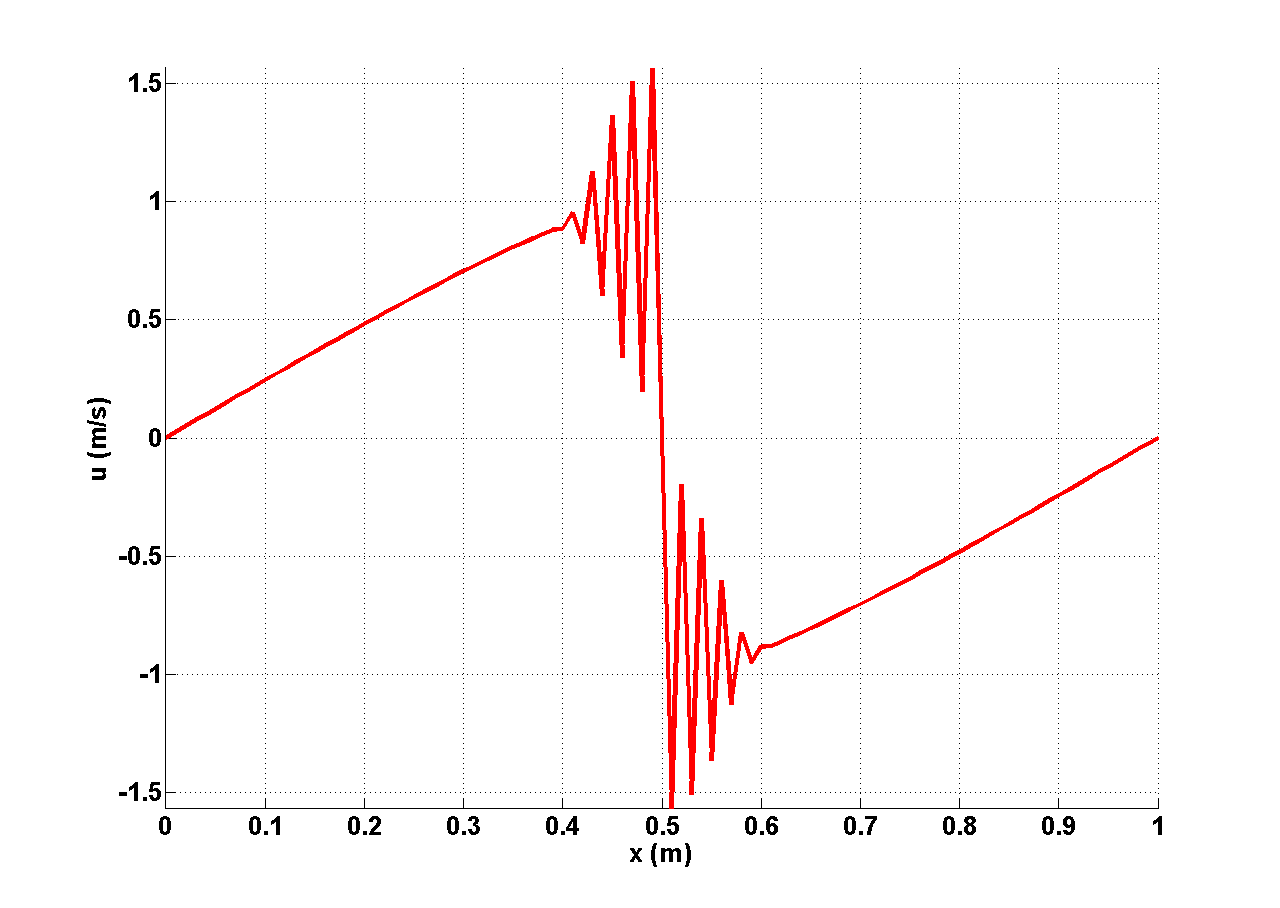
\includegraphics[width=\textwidth]{figures_burgers/1D_sol_free.png}
                %\caption{Without stabilization.}
        %\end{subfigure}%
        %\begin{subfigure}[b]{0.37\textwidth}
                %\centering
                %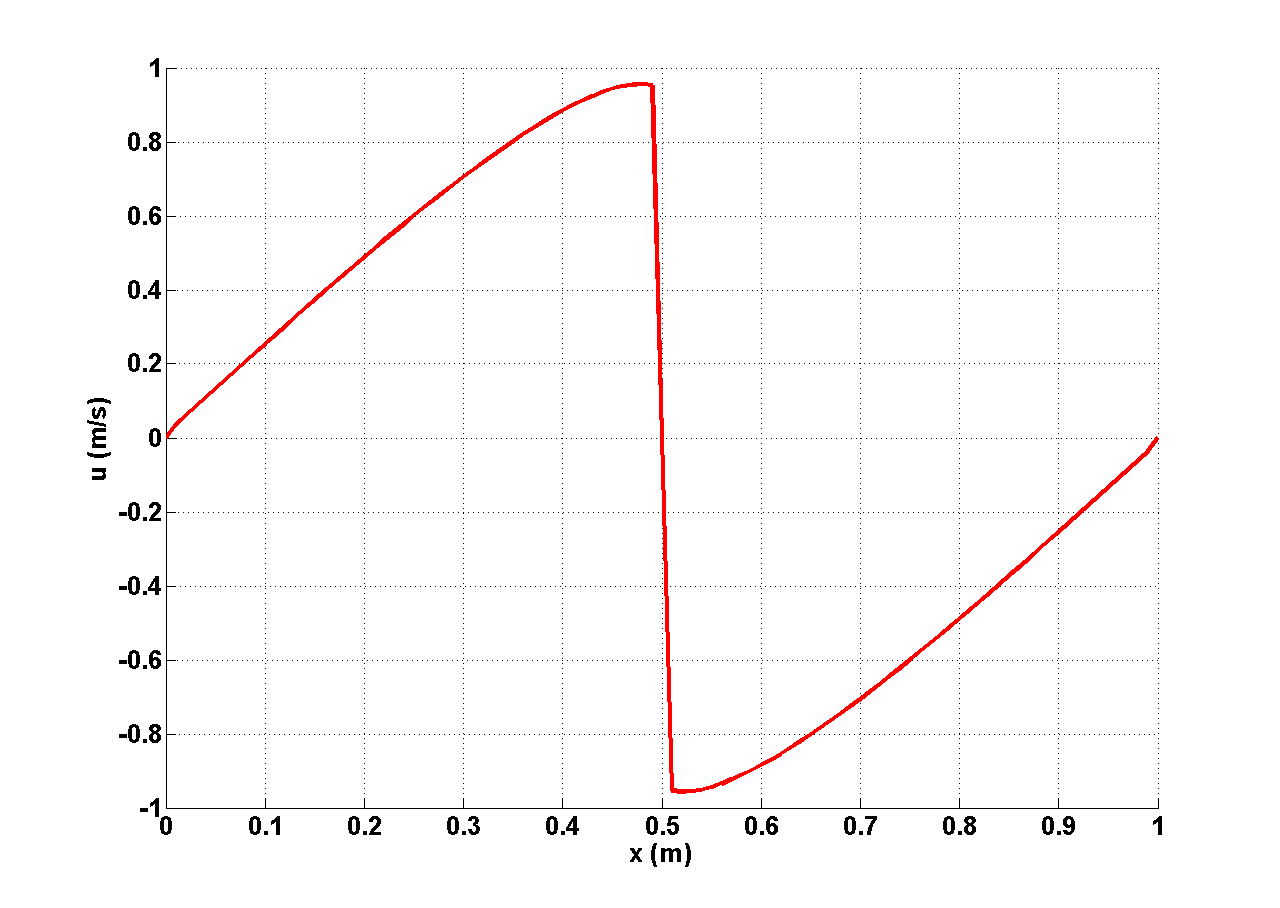
\includegraphics[width=\textwidth]{figures_burgers/1D_sol_fo.png}
                %\caption{With first-order viscosity.}
        %\end{subfigure}
        %
        %\begin{subfigure}[b]{0.37\textwidth}
                %\centering
                %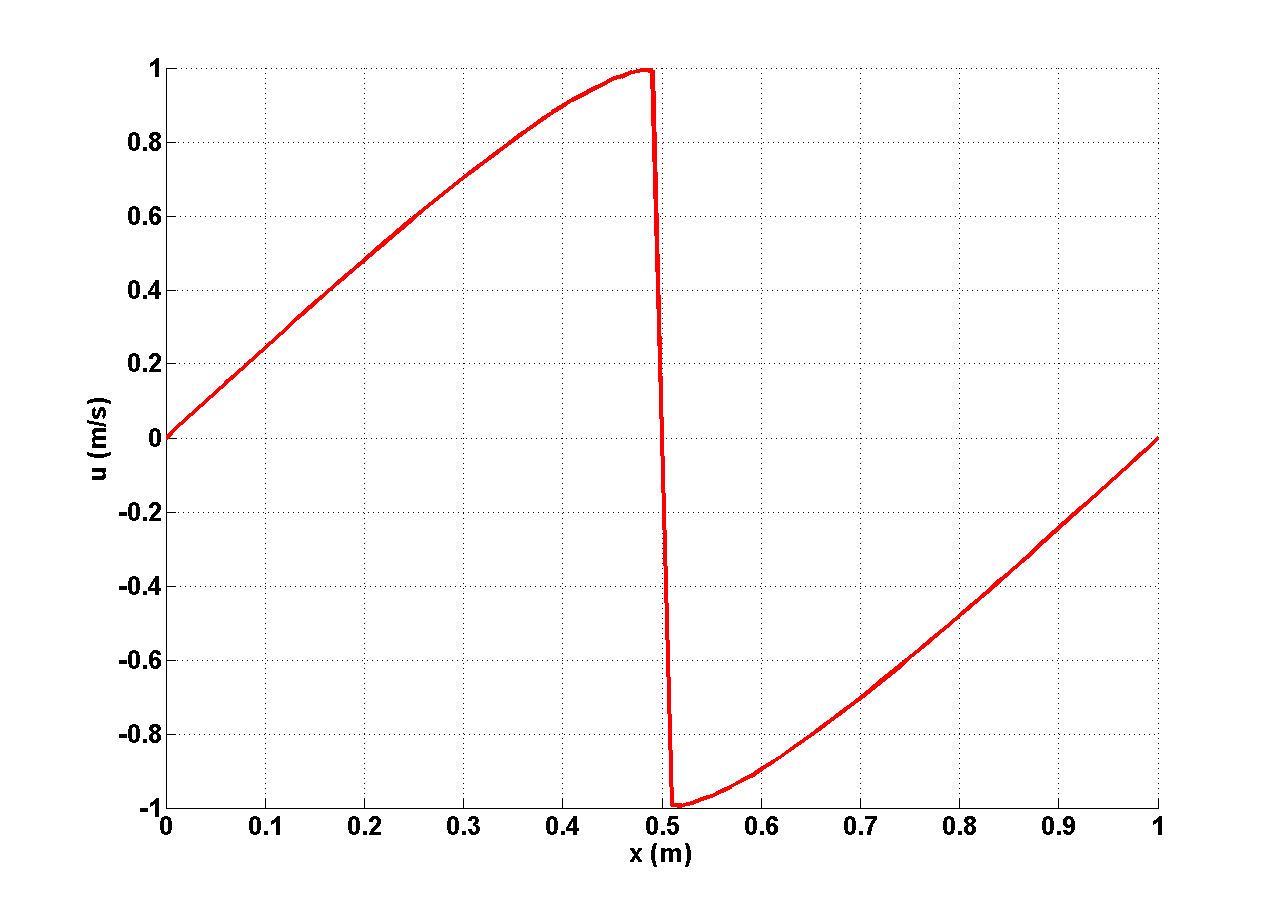
\includegraphics[width=\textwidth]{figures_burgers/1D_sol_ev.png}
                %\caption{With the EVM.}
        %\end{subfigure}
        %\begin{subfigure}[b]{0.37\textwidth}
                %\centering
                %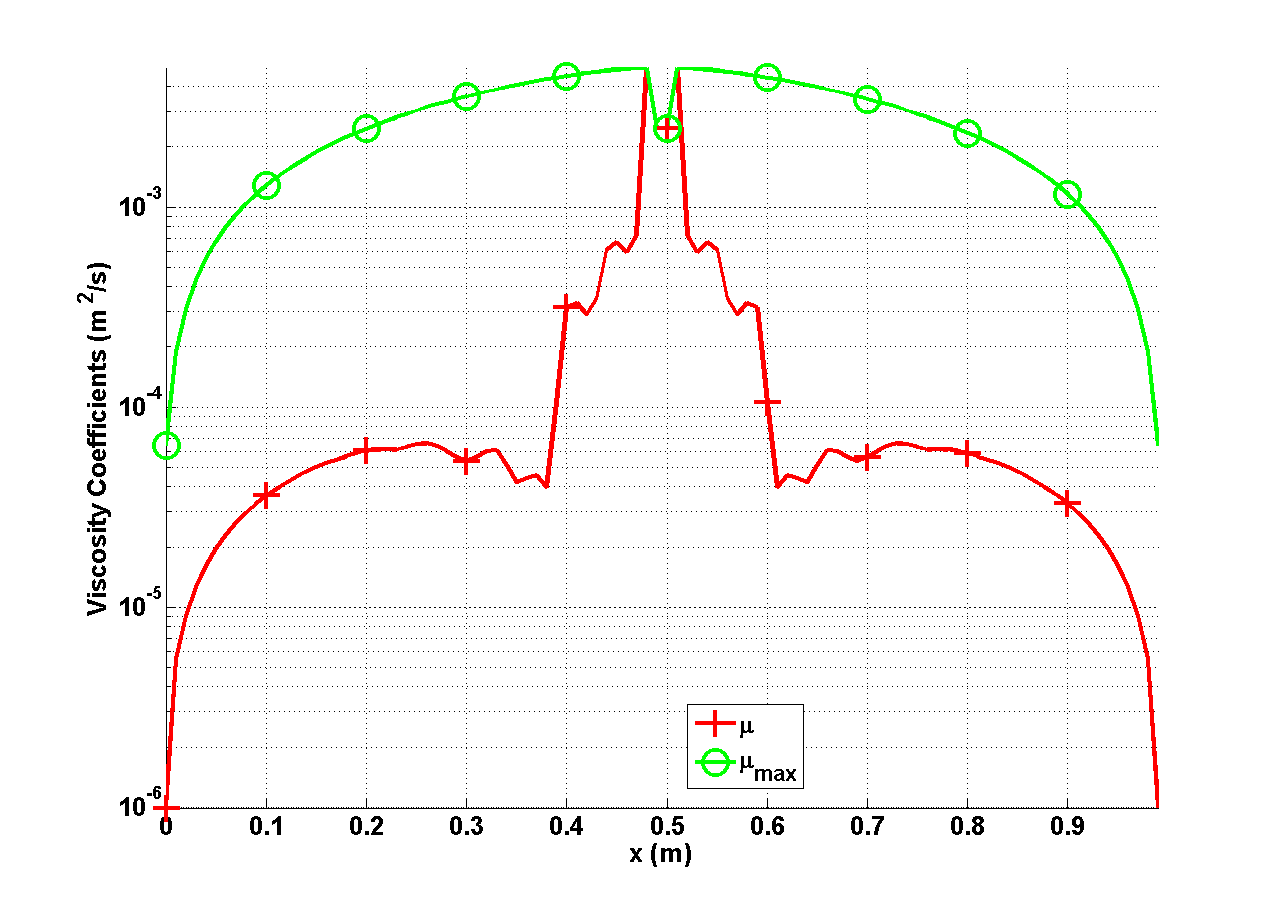
\includegraphics[width=\textwidth]{figures_burgers/1D_visc.png}
                %\caption{Viscosity coefficient profiles.}
        %\end{subfigure}
%\end{figure}
\vspace{-4mm}
\begin{figure}
\centering
\subfigure[Without stabilization]{
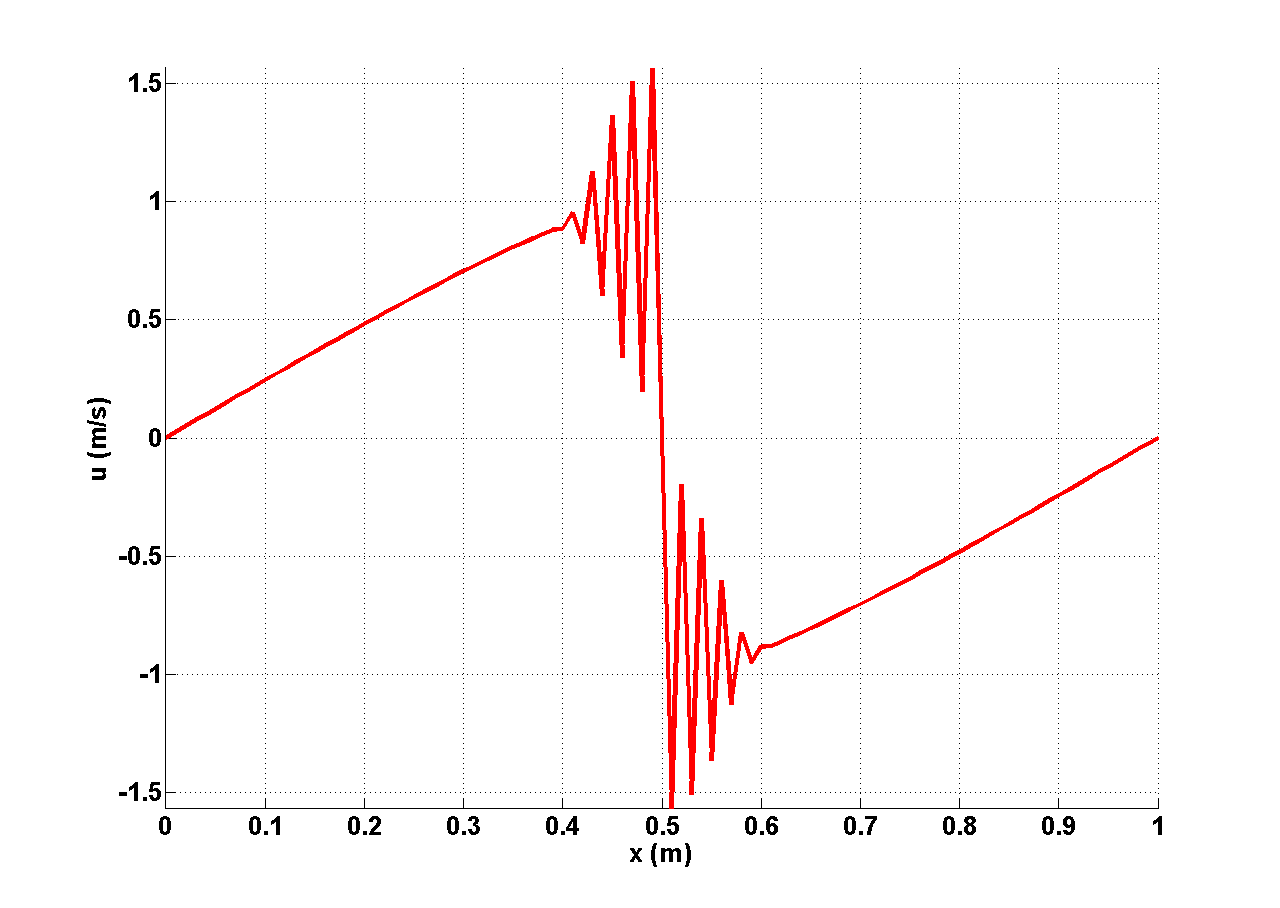
\includegraphics[width=0.4\textwidth]{figures_burgers/1D_sol_free.png}
}
\subfigure[With first-order viscosity]{
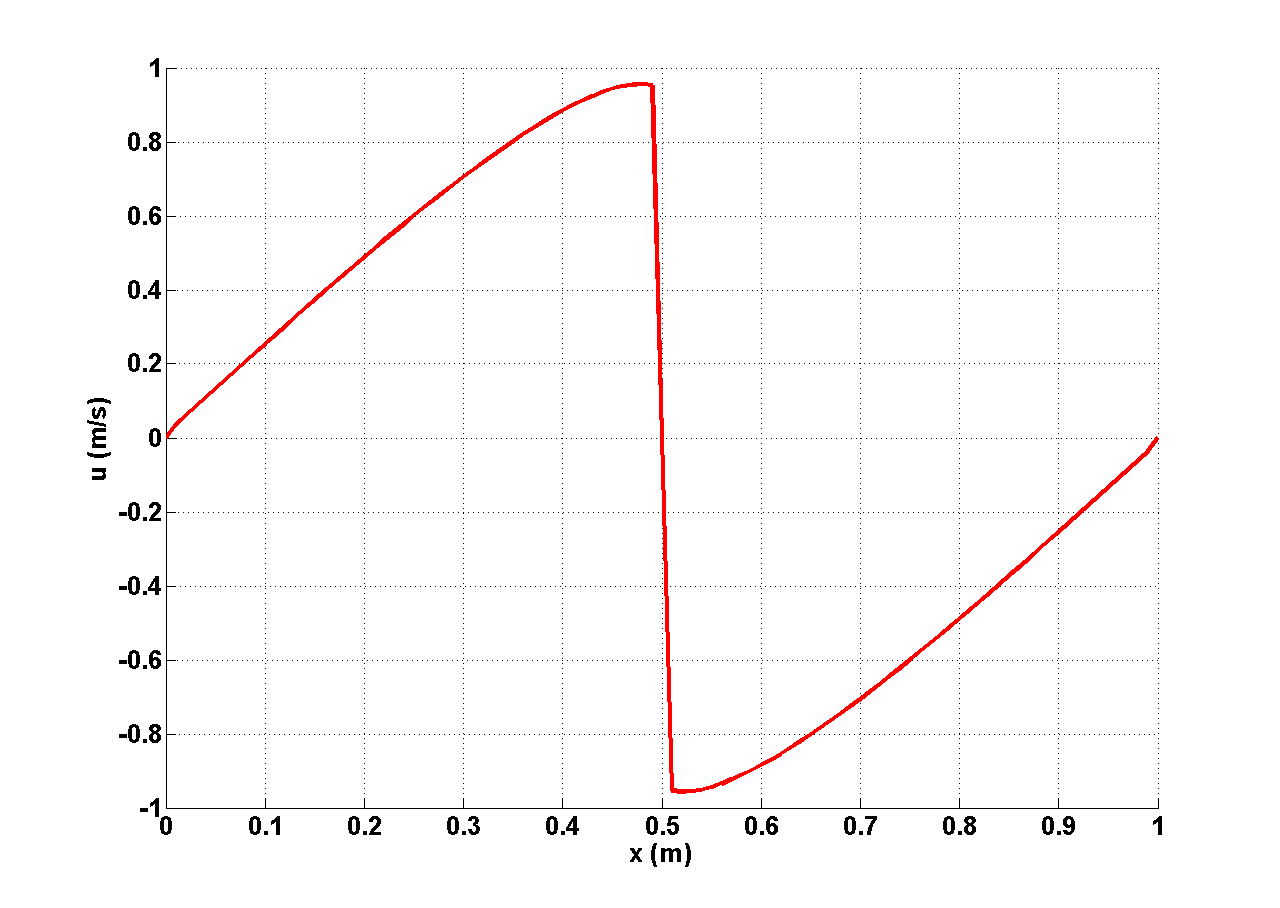
\includegraphics[width=0.4\textwidth]{figures_burgers/1D_sol_fo.png}
}
\subfigure[With entropy viscosity]{
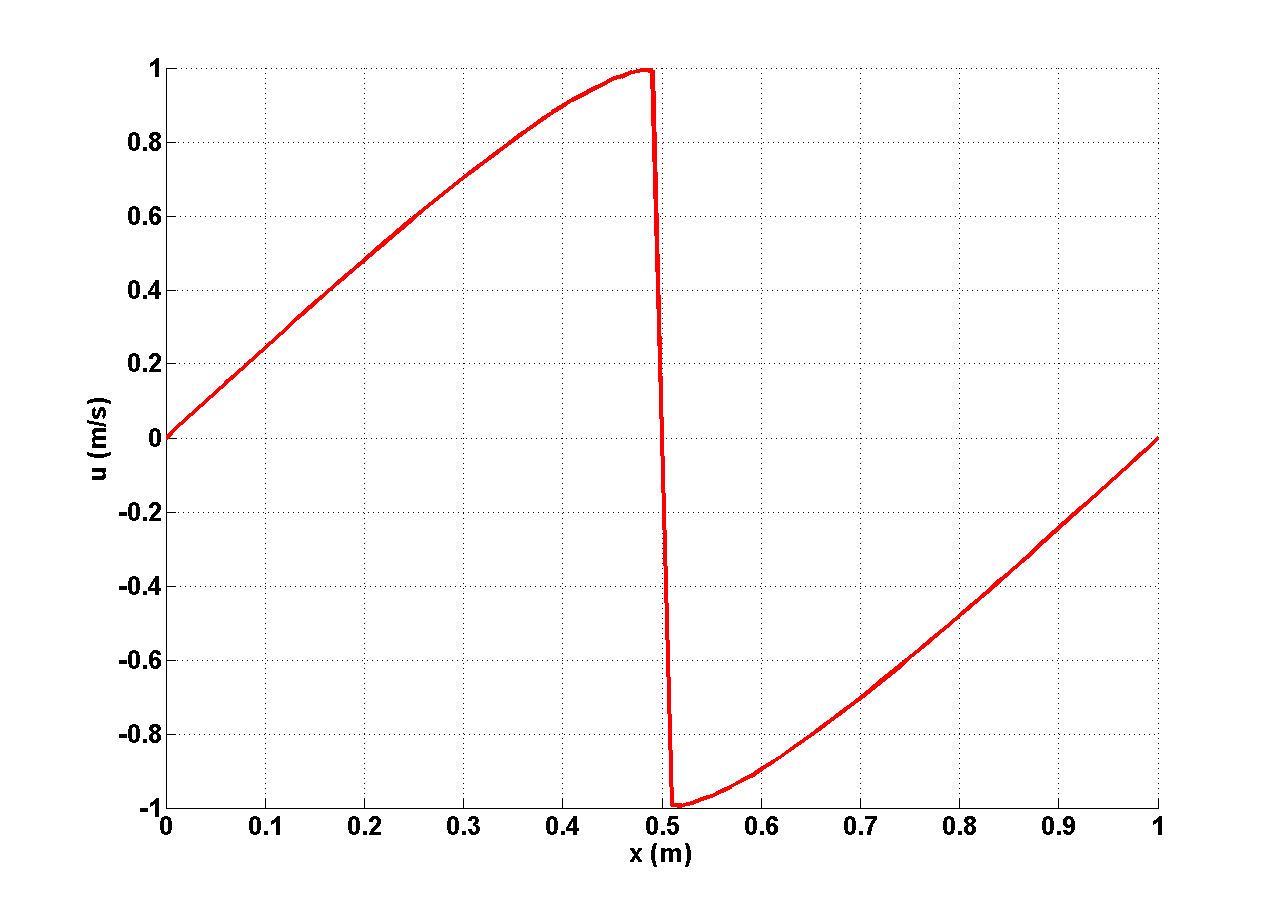
\includegraphics[width=0.4\textwidth]{figures_burgers/1D_sol_ev.png}
}
% \subfigure[Viscosity coefficient profiles \tcr{(log scale !!!)}]{
\subfigure[Viscosity coefficient profiles]{
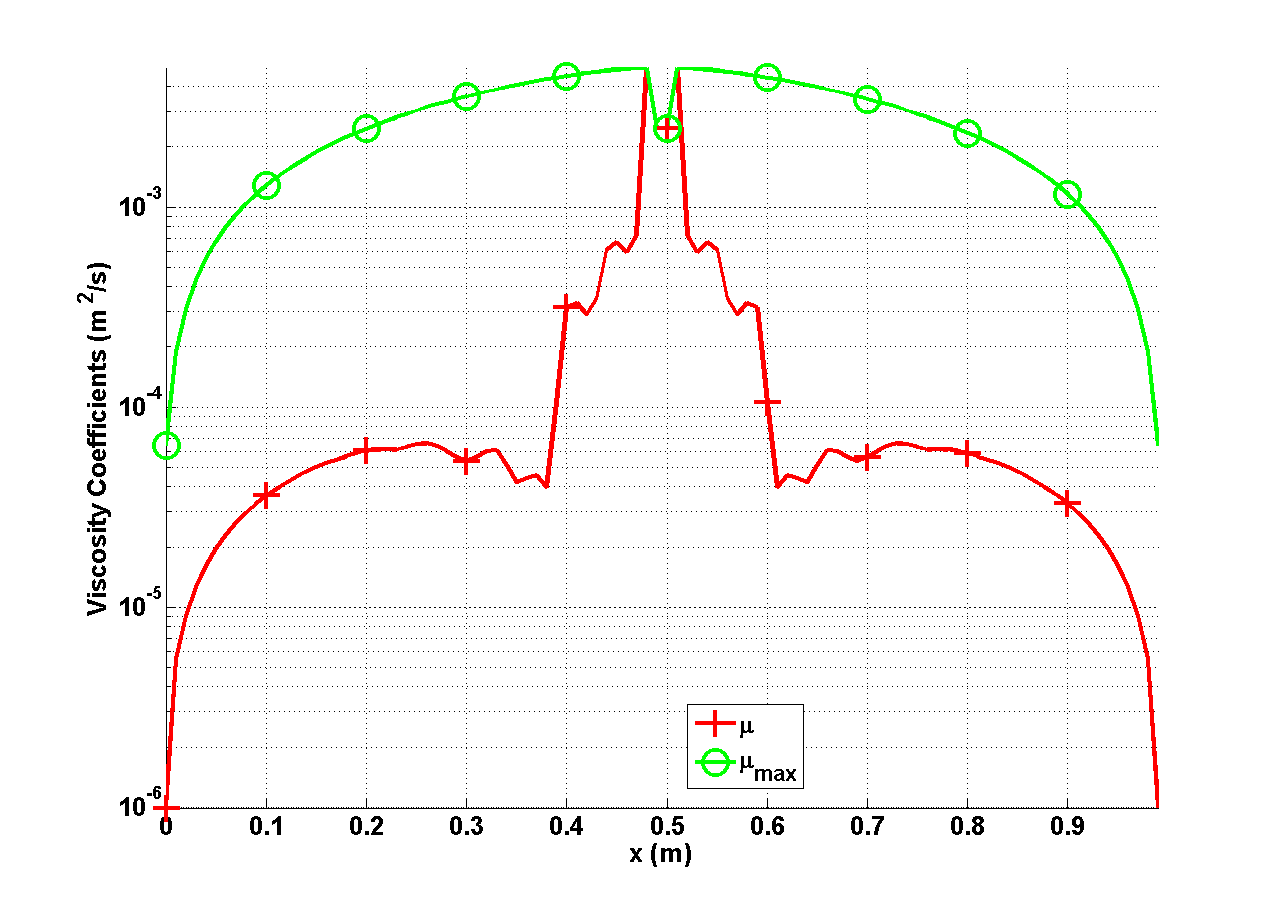
\includegraphics[width=0.4\textwidth]{figures_burgers/1D_visc.png}
}
\end{figure}

\end{frame}
%%%%%%%%%%%%%%%%%%%%%%%%%%%%%%%%%%%%%%%%%%%%%%%%%%%%%%%%%%%%%%%%%%%%

%%%%%%%%%%%%%%%%%%%%%%%%%%%%%%%%%%%%%%%%%%%%%%%%%%%%%%%%%%%%%%%%%%%%
\begin{frame}
\begin{figure}
	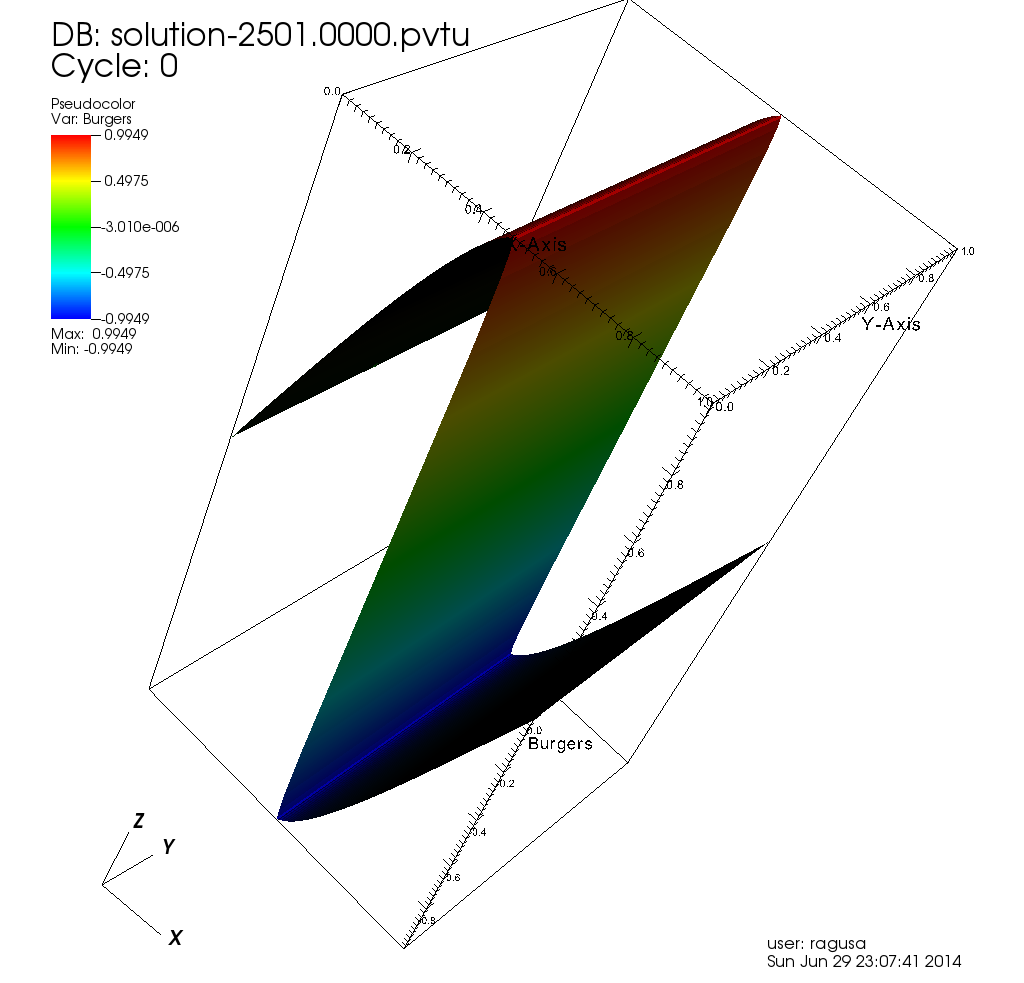
\includegraphics[height=7cm, keepaspectratio=true]{figures_burgers/burgers0000.png}
\end{figure}
\end{frame}
%%%%%%%%%%%%%%%%%%%%%%%%%%%%%%%%%%%%%%%%%%%%%%%%%%%%%%%%%%%%%%%%%%%%

%%%%%%%%%%%%%%%%%%%%%%%%%%%%%%%%%%%%%%%%%%%%%%%%%%%%%%%%%%%%%%%%%%%%%
%\begin{frame} 
%\begin{figure}
%	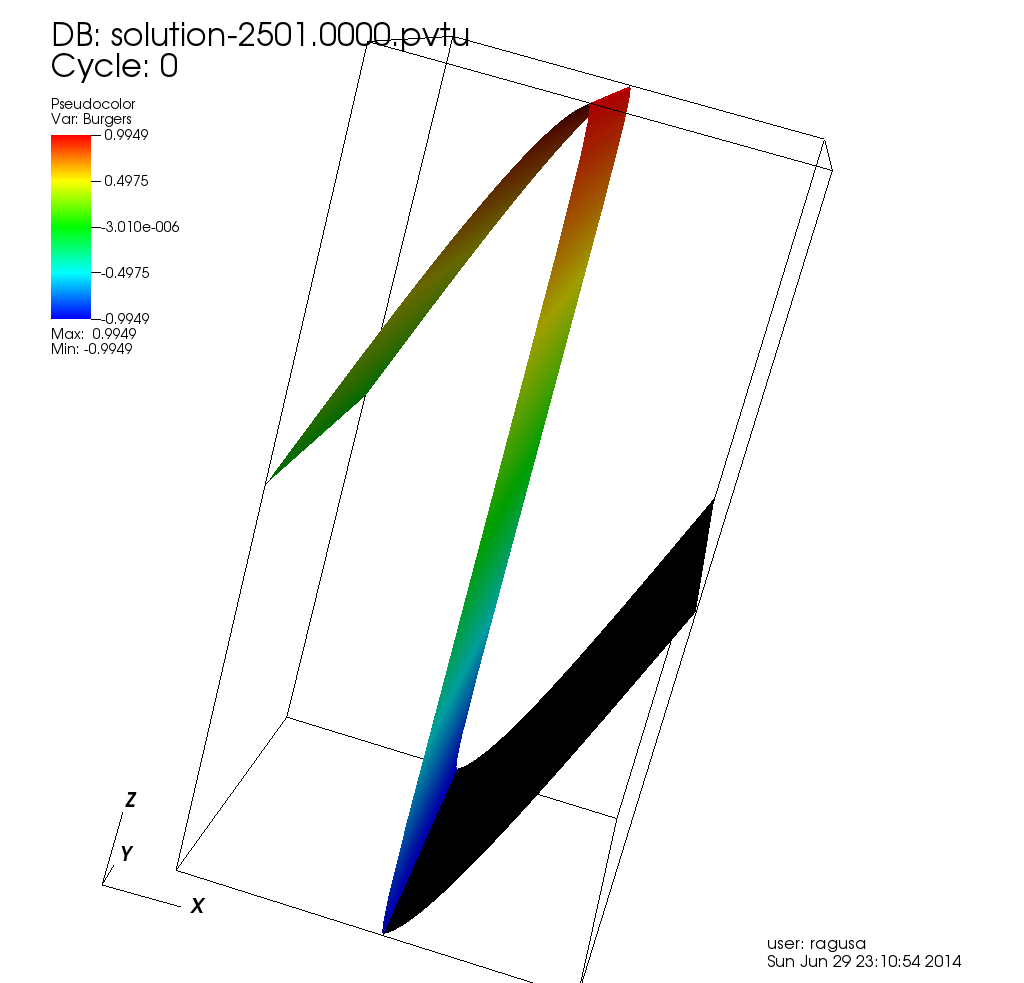
\includegraphics[height=7cm, keepaspectratio=true]{figures_burgers/burgers20000.png}
%\end{figure}
%\end{frame}
%%%%%%%%%%%%%%%%%%%%%%%%%%%%%%%%%%%%%%%%%%%%%%%%%%%%%%%%%%%%%%%%%%%%%

%%%%%%%%%%%%%%%%%%%%%%%%%%%%%%%%%%%%%%%%%%%%%%%%%%%%%%%%%%%%%%%%%%%%
%\subsection{Application to the Entropy Viscosity Method to the Euler Equations}
%%%%%%%%%%%%%%%%%%%%%%%%%%%%%%%%%%%%%%%%%%%%%%%%%%%%%%%%%%%%%%%%%%%%

%%%%%%%%%%%%%%%%%%%%%%%%%%%%%%%%%%%%%%%%%%%%%%%%%%%%%%%%%%%%%%%%%%%%
%************************************************
%\subsection{Entropy-viscosity method: original supersonic formulation}
%%************************************************

%%%%%%%%%%%%%%%%%%%%%%%%%%%%%%%%%%%%%%%%%%%%%%%%%%%%%%%%%%%%%%%%%%%%
\begin{frame}{Viscous regularization of Euler equations}

\begin{block}{\tcr{Regularized} Euler equations}
\begin{subequations}
\label{eq:euler_visc}
%
\begin{equation}
\partial_t \rho + \div \left( \rho \vec{u} \right) = \textcolor{red}{\div \vec{f}} \nonumber
\end{equation}
%
\begin{equation}
\partial_t \left( \rho \vec{u} \right) + \div \left( \rho \vec{u} \otimes \vec{u} + P \mathbb{I} \right) =  \textcolor{red}{\div \mathbb{g} }\nonumber
\end{equation}
%
\begin{equation}
\partial_t \left( \rho E  \right) + \div \left[ \vec{u} \left( \rho E + P \right) \right] = \textcolor{red}{\div \vec{h} }\nonumber
\end{equation}
\end{subequations}

\smallskip

How to select the \tcr{artificial viscous fluxes}?

\smallskip

By proving that the \tcr{regularized} equations satisfy a minimum principle on the specific entropy, \tcr{$s(\rho,e)$}  \tcb{[Guermond/Popov/Pasquetti (JCP 2011)]}

\end{block}

\begin{block}{Minimum entropy principle}
\be
\inf_{x\in \mathbb{R}^d} s(x,t) \ge \inf_{x\in \mathbb{R}^d} s_0(x) \qquad \forall t \ge 0
\ee
\end{block}

\end{frame}
%%%%%%%%%%%%%%%%%%%%%%%%%%%%%%%%%%%%%%%%%%%%%%%%%%%%%%%%%%%%%%%%%%%%


%%%%%%%%%%%%%%%%%%%%%%%%%%%%%%%%%%%%%%%%%%%%%%%%%%%%%%%%%%%%%%%%%%%%
\begin{frame}{General idea of the derivation}
%
\vspace{-1mm}
\begin{block}{Goal: To obtain an entropy relationship: $\rho ( \partial_t s + \vec{u} \cdot \grad s ) = \ldots  \tcr{\ge 0}$}
%Entropy is a function of density $\rho$ and internal energy $e$. Using chain rule, we have
\[
s=s(\rho,e) \quad \longrightarrow \quad \partial_\alpha s = s_\rho \tcr{\partial_\alpha \rho} + s_e \tcr{\partial_\alpha e} \quad \text{ with } \alpha={t,x} \ \text{(chain rule)} 
\]
%Obtain the entropy equation (re-write Euler equations in non-conservative form as a function of $\rho$, $u$, and $e$)
\end{block}
%
\vspace{-1mm}
\begin{block}{Entropy equation}
%Use chain rule and the mass and internal energy equations to get:
The following choice of \tcr{viscous fluxes}, $\vec{f} = \kappa \grad \rho$, $\mathbb{g} = \mu \rho \grad^s \vec{u} + \vec{u}\otimes \vec{f}$,and $\vec{h} = \kappa \grad(\rho e) -\tfrac{1}{2}u^2 \vec{f} + \mathbb{g}\cdot \vec{u}$, yields:
\begin{equation}
\rho \left( \partial_t s + \mbold{u} \cdot \grad s \right) = 
\div \left( \rho \kappa \grad s \right) -  \kappa \rho \mathbf{Q} +  s_e \mu \grad^s \mbold{u} : \grad \mbold{u}\nonumber
\end{equation}
\tcr{Viscosities} $\kappa$ and $\mu$ $\propto R_e := \partial_t s + \vec{u} \cdot \grad s$
\end{block}
%
\vspace{-1mm}
\begin{block}{Quadratic form}
\begin{equation}
\mathbf{Q} = X^t \mathbb{\Sigma} X 
\quad \text{ with } 
X = 
\begin{bmatrix}
\grad \rho \\
\grad e 
\end{bmatrix}
\text{ and } 
\mathbb{\Sigma} = 
\begin{bmatrix}
       \partial_{\rho} (\rho^2 \partial_{\rho} s) & \partial_{\rho,e} s  \\[0.3em]
       \partial_{\rho,e} s & \partial_{e,e} s           \\[0.3em]
\end{bmatrix} \nonumber 
\end{equation}
The form $\mathbf{Q}$ is negative definite if and only if $-s$ is convex with respect to $e$ and $\rho^{-1}$.
\end{block}
%
\vspace{-1mm}
\tcr{QED}  \ \ (recall: $s_e = 1/T > 0 $)

\end{frame}
%%%%%%%%%%%%%%%%%%%%%%%%%%%%%%%%%%%%%%%%%%%%%%%%%%%%%%%%%%%%%%%%%%%%

%\end{document}
%%%%%%%%%%%%%%%%%%%%%%%%%%%%%%%%%%%%%%%%%%%%%%%%%%%%%%%%%%%%%%%%%%%%
\begin{frame}
\begin{block}{Euler equations with viscous regularization (final form)}
\begin{subequations}
%
%\text{Continuity equation:}
\begin{equation}
\partial_t \rho + \div \left( \rho \vec{u} \right) = \textcolor{red}{\div \left( \kappa  \grad \rho \right)} \nonumber
\end{equation}
%
%\text{Momentum equation:}
\begin{equation}
\partial_t \left( \rho \vec{u} \right) + \div \left( \rho \vec{u} \otimes \vec{u} + P \mathbb{I} \right) =  \textcolor{red}{\div \left( \mu \rho  \grad^s \vec{u}  + \kappa \vec{u} \otimes \grad \rho \right) }\nonumber
\end{equation}
%
%\text{Energy equation:}
\begin{equation}
\partial_t \left( \rho E  \right) + \div \left[ \vec{u} \left( \rho E + P \right) \right] = \textcolor{red}{\div \left( \kappa \grad \left( \rho e \right) + \frac{1}{2}|| \vec{u} ||^2 \kappa \grad \rho +  \rho \mu \vec{u} \grad \vec{u}  \right) }\nonumber
\end{equation}
\end{subequations}

\smallskip

where $\kappa$ and $\mu$ are positive viscosity coefficients.
\end{block}

\begin{block}{Definition of the viscosity coefficients}
\begin{itemize}
\item As before, $\mu = \min(\mu^{LLF}, \mu^{\textit{entr}})$ and $\kappa = \min (\kappa^{LLF}, \kappa^{\textit{entr}})$ 
\item Entropy viscosities \tcr{$\propto$ entropy production}
\item All-speed (from low-Mach to supersonic) extension by \tcb{Delchini/Ragusa/Berry in Computers \& Fluids, 2015} 
%%\item
%%Note that if $\mu = \kappa$ (and one selects $\grad \vec{u} $ instead of $\grad^s \vec{u} $), we recover a parabolic regularization (on $\rho$, $\rho \vec{u}$, and $\rho E$).
\end{itemize}
\end{block}

%\begin{block}{}
%\hspace{0.5cm} $\bullet$ Multi-wave problem: $\lambda_1 = \vec{u} \cdot \vec{n} - c $, $\lambda_2 = \vec{u} \cdot \vec{n} + c $ and $\lambda_{3, \dots, 3+D} = \vec{u} \cdot \vec{n}$. \\
%\hspace{0.5cm} $\bullet$ $\kappa$ and $\mu$ are two positive viscosity coefficients.
%\end{block}
\end{frame}
%%%%%%%%%%%%%%%%%%%%%%%%%%%%%%%%%%%%%%%%%%%%%%%%%%%%%%%%%%%%%%%%%%%%

%%%%%%%%%%%%%%%%%%%%%%%%%%%%%%%%%%%%%%%%%%%%%%%%%%%%%%%%%%%%%%%%%%%%%
\begin{frame}{Leblanc shock tube}
\setcounter{subfigure}{0}% Reset subfigure counter
\vspace{-5mm}
\begin{figure}[H]
\centering
\subfigure[Density]{
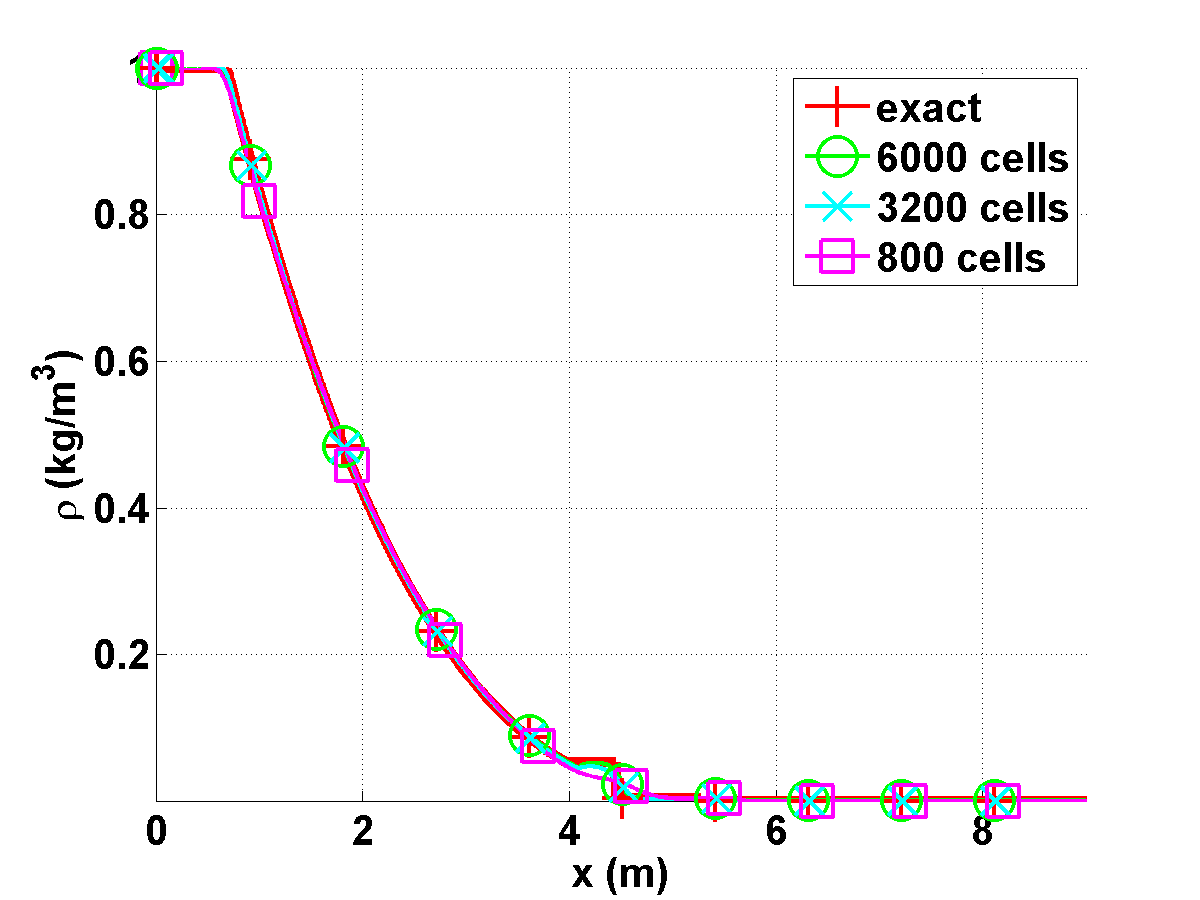
\includegraphics[width=0.4\textwidth]{figures_leblanc/Leblanc_exact_and_numerical_stt_density_6000.png}
}
\subfigure[Momentum]{
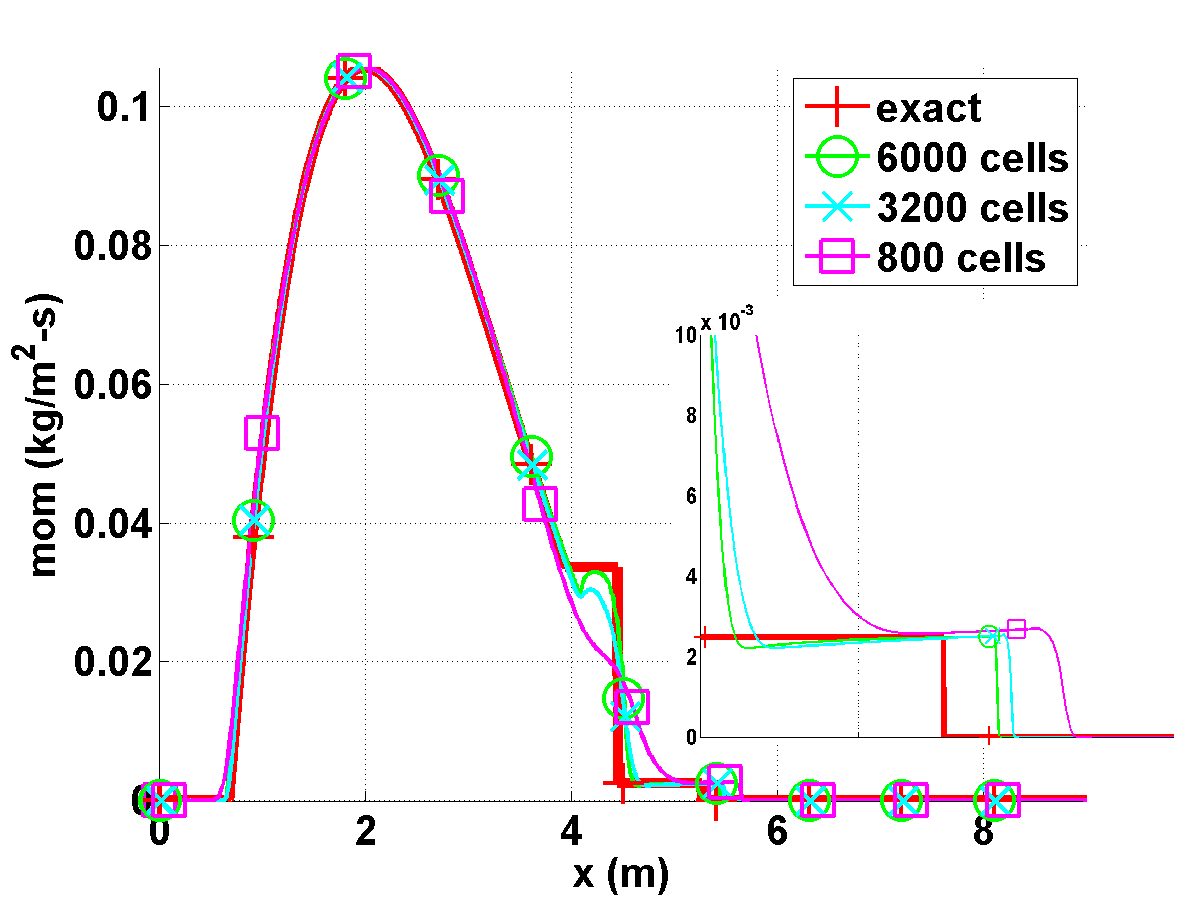
\includegraphics[width=0.4\textwidth]{figures_leblanc/Leblanc_exact_and_numerical_stt_momentum_6000.png}
}
\subfigure[Total energy]{
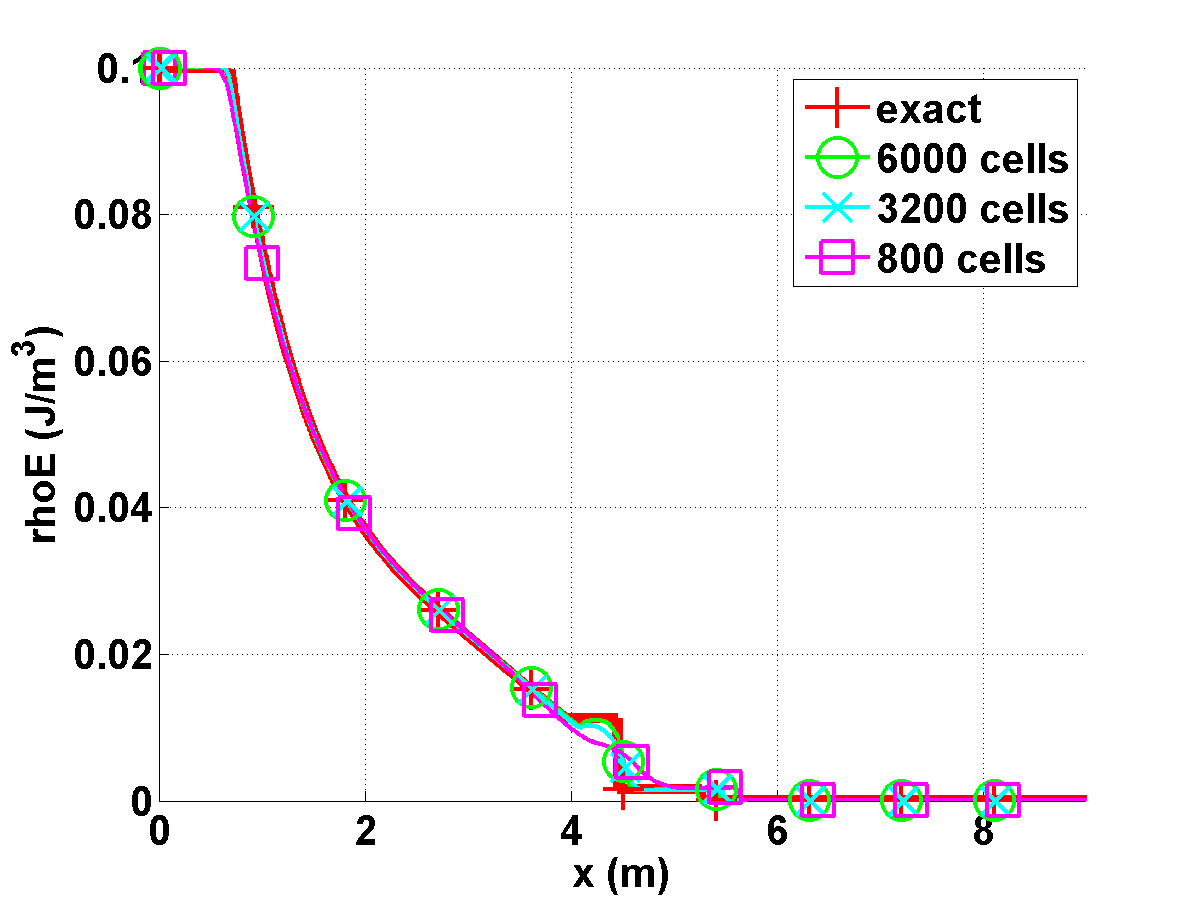
\includegraphics[width=0.4\textwidth]{figures_leblanc/Leblanc_exact_and_numerical_stt_total_energy_6000.png}
}
\subfigure[Viscosity]{
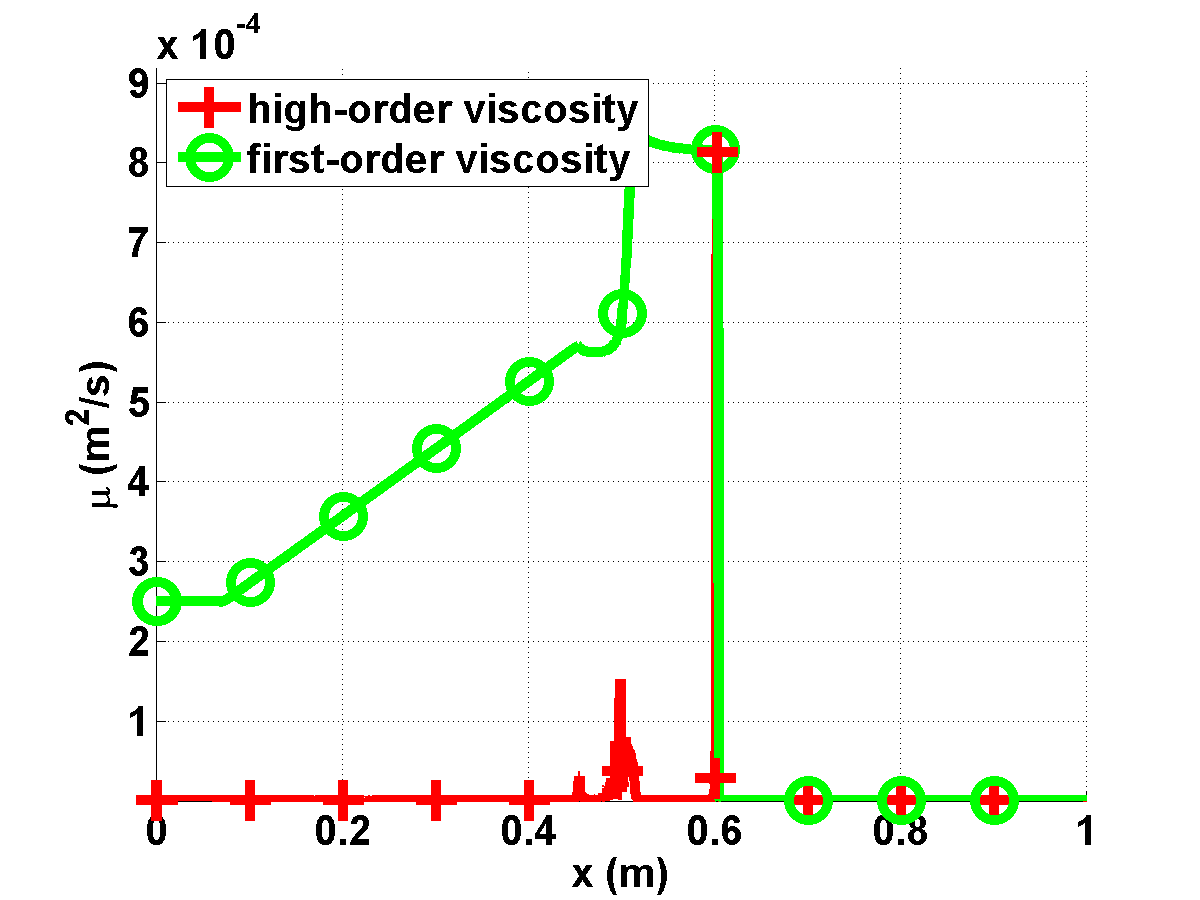
\includegraphics[width=0.4\textwidth]{figures_leblanc/Leblanc_viscosity_numerical_6000.png}
}
\end{figure}
\end{frame}
%%%%%%%%%%%%%%%%%%%%%%%%%%%%%%%%%%%%%%%%%%%%%%%%%%%%%%%%%%%%%%%%%%%%%

%%%%%%%%%%%%%%%%%%%%%%%%%%%%%%%%%%%%%%%%%%%%%%%%%%%%%%%%%%%%%%%%%%%%%
\begin{frame}{2-D explosion test}
\setcounter{subfigure}{0}% Reset subfigure counter
\begin{figure}[H]
\centering
\subfigure[Density]{
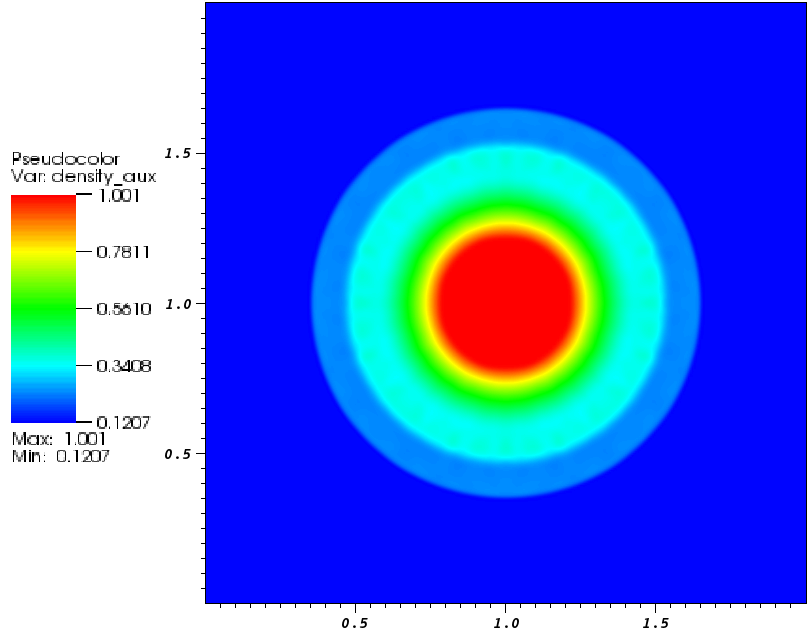
\includegraphics[width=0.48\textwidth]{figures_more_euler/Explosion_density_profiles.png}
}
\subfigure[Viscosity]{
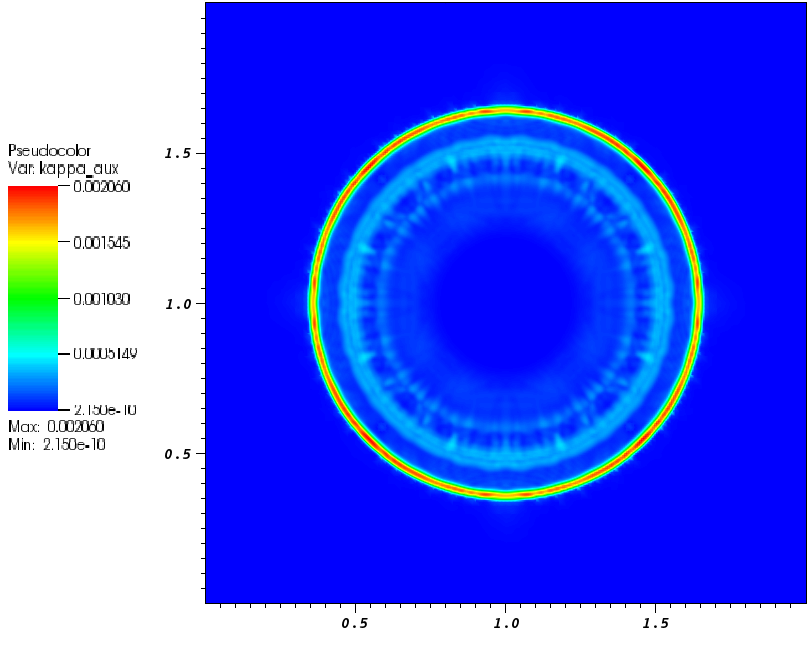
\includegraphics[width=0.48\textwidth]{figures_more_euler/Explosion_viscosity_profiles.png}
}
\end{figure}
\end{frame}
%%%%%%%%%%%%%%%%%%%%%%%%%%%%%%%%%%%%%%%%%%%%%%%%%%%%%%%%%%%%%%%%%%%%%

%%%%%%%%%%%%%%%%%%%%%%%%%%%%%%%%%%%%%%%%%%%%%%%%%%%%%%%%%%%%%%%%%%%%%
%\begin{frame}{Euler example: Mach-3 forward facing step}
%
%\begin{center}
%\movie[width=6cm,height=4cm,showcontrols=true,externalviewer]{\includegraphics[width=6cm,height=4cm]{engr.pdf}}{movs/forward_facing_step_density_movie.mpeg}\\
%\end{center}
%
%\begin{center}
%\begin{columns}
%\column{.5\textwidth}
%\includemedia[addresource=compression_corner.mp4, activate=pageopen, deactivate=pageclose, width=6.5cm, height=5cm, flashvars={source=mov/compression_corner.mp4 & autoPlay=true & loop=true }]{}{VPlayer.swf}
%\column{.5\textwidth}
%\includemedia[addresource=compression_corner_viscosity.mp4, activate=pageopen, deactivate=pageclose, width=6.5cm, height=5cm, flashvars={source=mov/compression_corner_viscosity.mp4 & autoPlay=true & loop=true }]{}{VPlayer.swf}
%\end{columns}
%\end{center}
%
%
%\end{frame}
%%%%%%%%%%%%%%%%%%%%%%%%%%%%%%%%%%%%%%%%%%%%%%%%%%%%%%%%%%%%%%%%%%%%%
%
%%%%%%%%%%%%%%%%%%%%%%%%%%%%%%%%%%%%%%%%%%%%%%%%%%%%%%%%%%%%%%%%%%%%%
%\begin{frame}{Mach-3 forward facing step: density contour}
%
%\begin{center}
%\movie[width=6cm,height=4cm,showcontrols=true,externalviewer]{\includegraphics[width=6cm,height=4cm]{engr.pdf}}{movs/forward_facing_step_density_movie.mpeg}\\
%\end{center}
%
%\end{frame}
%%%%%%%%%%%%%%%%%%%%%%%%%%%%%%%%%%%%%%%%%%%%%%%%%%%%%%%%%%%%%%%%%%%%%
%
%%%%%%%%%%%%%%%%%%%%%%%%%%%%%%%%%%%%%%%%%%%%%%%%%%%%%%%%%%%%%%%%%%%%%
%\begin{frame}{Mach-3 forward facing step: viscosity contour}
%
%\begin{center}
%\movie[width=6cm,height=4cm,showcontrols=true,externalviewer]{\includegraphics[width=6cm,height=4cm]{engr.pdf}}{movs/forward_facing_step_viscosity.mpeg}\\
%\end{center}
%
%\end{frame}
%%%%%%%%%%%%%%%%%%%%%%%%%%%%%%%%%%%%%%%%%%%%%%%%%%%%%%%%%%%%%%%%%%%%%
%
%%%%%%%%%%%%%%%%%%%%%%%%%%%%%%%%%%%%%%%%%%%%%%%%%%%%%%%%%%%%%%%%%%%%
%%%%%%%%%%%%%%%%%%%%%%%%%%%%%%%%%%%%%%%%%%%%%%%%%%%%%%%%%%%%%%%%%%%%
\subsection{Entropy-based artificial viscosity for the GRH}
%%%%%%%%%%%%%%%%%%%%%%%%%%%%%%%%%%%%%%%%%%%%%%%%%%%%%%%%%%%%%%%%%%%%
%%%%%%%%%%%%%%%%%%%%%%%%%%%%%%%%%%%%%%%%%%%%%%%%%%%%%%%%%%%%%%%%%%%%

%%%%%%%%%%%%%%%%%%%%%%%%%%%%%%%%%%%%%%%%%%%%%%%%%%%%%%%%%%%%%%%%%%%%%
%\subsubsection{Questions to answer}
%%%%%%%%%%%%%%%%%%%%%%%%%%%%%%%%%%%%%%%%%%%%%%%%%%%%%%%%%%%%%%%%%%%%%

%%%%%%%%%%%%%%%%%%%%%%%%%%%%%%%%%%%%%%%%%%%%%%%%%%%%%%%%%%%%%%%%%%%%
\begin{frame}
%{Entropy-based artificial viscosity technique for the GRH}
\vspace{-2mm}
\begin{block}{Entropy viscosity for the GRH: questions to answer}
\begin{enumerate}
\item 
The GRHD equations are \tcr{not hyperbolic}. Can we apply the entropy viscosity method (EVM)?
\begin{itemize}
\item Our initial attempt [\tcb{JCP 2015}]: apply the EVM to the hyperbolic part of the GRHD [an idea similar to \tcb{Balsara JQSRT 1999}, \tcb{Lowrie\&Morel JQSRT 2001}]
\end{itemize}
\item
What is an appropriate functional form for the entropy of the GRHD, $\tcr{s(\rho,e,\epsilon) = \ldots}$\tcr{???} 
\item
What is an appropriate expression for the viscous fluxes so that the \tcr{regularized} GRHD eqs satisfy 
the minimum entropy principle?
\item
Is the viscous regularization well-behaved in the \tcr{equilibrium-diffusion limit}?
\end{enumerate}
\end{block}
\vspace{-4mm}
\begin{columns}
    \begin{column}{0.7\textwidth}

\begin{block}{Hyperbolic part of the GRHD}
%[an idea similar to \tcb{Balsara JQSRT 1999}, \tcb{Lowrie\&Morel JQSRT 2001}]
\begin{subequations}
\begin{equation}
\partial_t \left( \rho \right) + \partial_x\left( \rho u \right) = 0 
\end{equation}
%
\begin{equation}
\partial_t \left( \rho u\right) + \partial_x \left(\rho u^2 + P + \frac{\epsilon}{3} \right) = 0 
\end{equation}
%
\begin{equation}
\partial_t \left( \rho E\right) + \partial_x \left[ u \left( \rho E + P \right) \right] +\frac{u}{3} \partial_x \epsilon = 0
\end{equation}
%
\begin{equation}
\partial_t \epsilon + \frac{4}{3} \partial_x \left( u \epsilon \right) - \frac{u}{3} \partial_x \epsilon = 0
\end{equation}
\end{subequations}
\end{block}

    \end{column}
    \begin{column}{0.3\textwidth}

        \begin{block}{Eigenvalues}
\begin{align*}
\lambda_{1,4} &= u\pm c_m \\
\lambda_{2,3} &= u     
\end{align*}
with
\begin{equation*}
c_m^2 = \underbrace{P_{\rho} + \frac{P}{\rho^2}P_e}_{c_{Euler}^2} + \underbrace{\frac{4 \epsilon}{9\rho}}_{c^2_{rad}} 
\end{equation*}
        \end{block}

    \end{column}
\end{columns}

\end{frame}
%%%%%%%%%%%%%%%%%%%%%%%%%%%%%%%%%%%%%%%%%%%%%%%%%%%%%%%%%%%%%%%%%%%%

%%%%%%%%%%%%%%%%%%%%%%%%%%%%%%%%%%%%%%%%%%%%%%%%%%%%%%%%%%%%%%%%%%%%%
%\subsection{Previous results (JCP 2015)}
%%%%%%%%%%%%%%%%%%%%%%%%%%%%%%%%%%%%%%%%%%%%%%%%%%%%%%%%%%%%%%%%%%%%%
%

%%%%%%%%%%%%%%%%%%%%%%%%%%%%%%%%%%%%%%%%%%%%%%%%%%%%%%%%%%%%%%%%%%%%
\begin{frame}{Entropy-based artificial viscosity for the GRH: derivation}

\begin{block}{Study of the hyperbolic parts of the GRH: process}
\begin{enumerate}
\item Add viscous regularization (fluxes) to the equations
\begin{subequations}
\begin{equation}
\partial_t \left( \rho \right) + \partial_x\left( \rho u \right) = \tcr{\partial_x f}
\end{equation}
%
\begin{equation}
\partial_t \left( \rho u\right) + \partial_x \left(\rho u^2 + P + \frac{\epsilon}{3} \right) = \tcr{\partial_x g }
\end{equation}
%
\begin{equation}
\partial_t \left( \rho E\right) + \partial_x \left[ u \left( \rho E + P \right) \right] +\frac{u}{3} \partial_x \epsilon = \tcr{\partial_x h  }
\end{equation}
%
\begin{equation}
\partial_t \epsilon + \frac{4}{3} \partial_x \left( u \epsilon \right) - \frac{u}{3} \partial_x \epsilon = \tcr{\partial_x \ell}
\end{equation}
\end{subequations}
\item With \tcr{$s(\rho,e,\epsilon)$}, use chain rule to obtain the entropy relationship
	\begin{equation}
		\partial_{\alpha} s = \partial_{\rho} s \partial_{\alpha} \rho +  \partial_{e} s \partial_{\alpha}e +  
		\partial_{\epsilon} s \partial_{\alpha} \epsilon 
	\end{equation} 
\item An observation: we can greatly simplify the expression by assuming \tcr{$s(\rho,e,\epsilon) = s_{Euler}(\rho,e) + s_{rad}(\rho,\epsilon)$}
%Use the viscous fluxes obtained for Euler's equations in the material equations (with $\kappa=\mu$), supplemented by an radiation energy viscous flux $\kappa \grad \epsilon$ 
\end{enumerate}
\end{block}

\end{frame}
%%%%%%%%%%%%%%%%%%%%%%%%%%%%%%%%%%%%%%%%%%%%%%%%%%%%%%%%%%%%%%%%%%%%

%%%%%%%%%%%%%%%%%%%%%%%%%%%%%%%%%%%%%%%%%%%%%%%%%%%%%%%%%%%%%%%%%%%%
\begin{frame}
\vspace{-2mm}
\begin{block}{Study of the hyperbolic parts of the GRHD: results}
\begin{enumerate}
\item
%After some tedious algebra, the following form of the entropy $s(\rho,e,\epsilon)$ is obtained
\begin{equation}
s(\rho, e, \epsilon) = s_{Euler}(\rho,e) + \frac{4 a^{1/4}}{3\rho} \epsilon^{\frac{3}{4}}
\end{equation}
\item Using the \tcr{Eulerian viscous fluxes}, supplemented by an \tcb{radiation energy viscous flux} 
%$\vec{\ell}=\kappa \grad \epsilon$  
\begin{equation}
\left\{
 \begin{array}{cl}
  \tcr{f}    &\tcr{= \kappa \partial_x \rho} \\
  \tcr{g}    &\tcr{= \rho \mu \partial_x u + uf} \\
  \tcr{h}    &\tcr{= \kappa \partial_x (\rho e) - \tfrac{1}{2} u^2 f + g u}\\
  \tcb{\ell} &\tcb{= \kappa \partial_x \epsilon}
 \end{array}
\right. 
\end{equation}
\item we get the following \tcm{entropy conservation statement}:
\begin{equation*}
\boxed{
\rho \frac{Ds}{Dt} = 
\partial_x \left( \rho \kappa \partial_x s \right) 
+ (\kappa \partial_x \rho) (\partial_x s )
- \rho \kappa X^T A X
+ s_e \rho \mu (\partial_x u)^2
\ \tcr{ \ge 0 }
}
\end{equation*} 
% where 
\begin{equation*}
X=
\begin{bmatrix}
 \partial_x \rho \\ \partial_x e \\ \partial_x \epsilon 
\end{bmatrix}
\text { and }
A = 
\begin{bmatrix}
\partial_{\rho} \left( \rho^2 \partial_{\rho} s_{Euler} \right) & \partial_{\rho,e} s_{Euler} & 0 \\
\partial_{\rho,e} s_{Euler} 									& \partial_{e,e} s_{Euler}    & 0 \\
0                           									&  0                          & -\frac{a^{1/4}}{4 \rho}\epsilon^{-5/4}
%0                           									&  0                          & \frac{\rho^{(0)}}{\rho} \partial_{\epsilon,\epsilon} \tilde{s}_{rad}
\end{bmatrix}
\end{equation*}
%\begin{equation}
%\boxed{\frac{Ds}{Dt} = \partial_t s + u \partial_x s \geq 0} 
%\end{equation}
\end{enumerate}
\end{block}
The form $X^T A X$ is negative -definite (\tcb{Delchini/Ragusa/Morel, JCP 2015})

\end{frame}
%%%%%%%%%%%%%%%%%%%%%%%%%%%%%%%%%%%%%%%%%%%%%%%%%%%%%%%%%%%%%%%%%%%%

%%%%%%%%%%%%%%%%%%%%%%%%%%%%%%%%%%%%%%%%%%%%%%%%%%%%%%%%%%%%%%%%%%%%%
%\subsection{Recent developments}
%%%%%%%%%%%%%%%%%%%%%%%%%%%%%%%%%%%%%%%%%%%%%%%%%%%%%%%%%%%%%%%%%%%%%

%%%%%%%%%%%%%%%%%%%%%%%%%%%%%%%%%%%%%%%%%%%%%%%%%%%%%%%%%%%%%%%%%%%%
\begin{frame}{Recent developments}
\vspace{-2mm}
\begin{block}{Entropy conservation statement for the \underline{\tcr{\bf full}} GRHD equations}
Recently, we have been able to show:
\begin{multline} 
\rho \frac{Ds}{Dt} = 
\partial_x \left( \rho \kappa \partial_x s \right) 
+ (\kappa \partial_x \rho) (\partial_x s )
- \rho \kappa X^T A X
+ s_e \rho \mu (\partial_x u)^2 \\
+ \tcr{\Big( \rho s_\epsilon -s_e \Big)  \sigma_a c \left( a T^4 - \epsilon \right) +   \rho s_\epsilon \partial_x \left( \frac{c}{3 \sigma_t} \partial_x \epsilon \right)} \ \tcm{\geq 0} 
\end{multline}
where the terms in \tcr{red} are unconditionally entropy-producing (\tcb{unpublished, submitted})
\end{block}
%
\vspace{-2mm}
%
\begin{block}{Finally, the Regularized \tcm{full} GRHD equations are: (shown here with $\kappa=\mu$)}
%
\begin{subequations}
\begin{equation}
\partial_t \left( \rho \right) + \partial_x\left( \rho u \right) = \tcr{\partial_x \left( \kappa \partial_x \rho \right)} 
\end{equation}
%
\begin{equation}
\partial_t \left( \rho u\right) + \partial_x \left(\rho u^2 + P + \frac{\epsilon}{3} \right) = \tcr{\partial_x \left( \kappa \partial_x (\rho u) \right) }
\end{equation}
%
\begin{equation}
\partial_t \left( \rho E\right) + \partial_x \left[ u \left( \rho E + P \right) \right] = -\frac{u}{3} \partial_x \epsilon \tcb{- \sigma_a c \left( a T^4 - \epsilon \right)} + \tcr{\partial_x \left( \kappa \partial_x (\rho E)\right)}
\end{equation}
%
\begin{equation}
\partial_t \epsilon + \frac{4}{3} \partial_x \left( u \epsilon \right) = \frac{u}{3} \partial_x \epsilon + \tcm{\partial_x \left( \frac{c}{3 \sigma_t} \partial_x \epsilon \right)} \tcb{+ \sigma_a c \left( a T^4 - \epsilon \right) }+ \tcr{\partial_x \left( \kappa \partial_x \epsilon \right)}
\end{equation}
\end{subequations}
%
\end{block}


\end{frame}
%%%%%%%%%%%%%%%%%%%%%%%%%%%%%%%%%%%%%%%%%%%%%%%%%%%%%%%%%%%%%%%%%%%%

%%%%%%%%%%%%%%%%%%%%%%%%%%%%%%%%%%%%%%%%%%%%%%%%%%%%%%%%%%%%%%%%%%%%
\begin{frame}{Equilibrium Diffusion Limit}
\vspace{-3mm}
\begin{block}{non-dimensionalization:}
%
%\begin{multline*}
%\rho'   = \frac{\rho}{\rho_\infty}               , 
%u'      = \frac{u}{c_{m,\infty}}                 ,  
%P'      = \frac{P}{\rho_\infty c^2_{m,\infty}}   ,  
%\epsilon'= \frac{\epsilon}{a T_\infty^4 }        , 
%E'      = \frac{E}{c^2_{m,\infty} }              ,  
%\sigma_t'      = \frac{\sigma_t}{\sigma_{t,\infty} }              , \\
%\sigma_a'      = \frac{\sigma_a}{\sigma_{a,\infty} }              , 
%T'      = \frac{T}{T_\infty }              , 
%x' = \frac{x}{L_\infty}                      ,  
%t' = \frac{t}{L_\infty / c_{m,\infty}}       ,  
%\kappa' = \frac{\kappa}{\kappa_\infty}       
%\end{multline*}
\begin{subequations}
\begin{equation}
\partial_{t'} \left( \rho' \right) + \partial_{x'}\left( \rho' u' \right) =  \tcr{\Pe \partial_x \left( \kappa' \partial_{x'} \rho' \right) }
\end{equation}
%
\begin{equation}
\partial_{t'} \left( \rho' u'\right) + \partial_{x'} \left(\rho u^{2'} + P' + \tcb{\Re} \frac{\epsilon'}{3} \right) = \tcr{\Pe \partial_{x'} \left( \kappa' \partial_{x'} (\rho' u') \right)} 
\end{equation}
%
\vspace{-7mm}
\begin{multline}
\partial_{t'} \left( \rho' E'\right) + \partial_{x'} \left[ u' \left( \rho' E' + P' \right) \right] 
= 
-
\tcb{\Re} \frac{u'}{3} \partial_{x'} \epsilon' 
\\ 
- 
\Re \Us^{-1} \tcb{\Ls} \left( \sigma_t' - \tcb{\Lsi} \sigma_s' \right)  \left(T^{\prime,4} - \epsilon' \right) 
+ 
 \tcr{\Pe \partial_{x'} \left( \kappa' \partial_{x'} (\rho' E')\right)  }
\end{multline}
%
\vspace{-7mm}
\begin{multline}
\partial_{t'} \epsilon' + \frac{4}{3} \partial_{x'} \left( u' \epsilon' \right) 
= \frac{u'}{3} \partial_{x'} \epsilon' 
+ 
\tcb{\Ls^{-1} \Us^{-1}} \partial_{x'} \left( \frac{1}{3 \sigma_t'} \partial_{x'} \epsilon' \right) 
\\ + 
\tcb{\Us^{-1} \Ls} \left( \sigma_t' - \tcb{\Lsi} \sigma_s' \right) \left( T^{\prime,4} - \epsilon' \right) 
+ 
 \tcr{\Pe \partial_{x'} \left( \kappa' \partial_{x'} \epsilon' \right)}
\end{multline}
\end{subequations}
\end{block}
%%
\vspace{-2mm}
%%
\begin{block}{non-dimensional parameters}
\begin{multline*}
\Ls = L_{\infty} \sigma_{t,\infty}                   =\mathcal{O}(\varepsilon^{-1})  , \  
\Lsi = \frac{\sigma_{s,\infty}}{\sigma_{t,\infty}} =\mathcal{O}(\varepsilon)    , \ 
\Us = \frac{c_{m,\infty}}{c}                       =\mathcal{O}(\varepsilon)   \\
\Re = \frac{a T^4_{\infty}}{\rho_{\infty} c^2_{m,\infty}}=\mathcal{O}(1)    , \ 
 \tcr{\Pe = \frac{\kappa_{\infty}}{c_{m,\infty} L_{\infty}}} =\mathcal{O}(1)   
\end{multline*}
\end{block}

\end{frame}
%%%%%%%%%%%%%%%%%%%%%%%%%%%%%%%%%%%%%%%%%%%%%%%%%%%%%%%%%%%%%%%%%%%%

%%%%%%%%%%%%%%%%%%%%%%%%%%%%%%%%%%%%%%%%%%%%%%%%%%%%%%%%%%%%%%%%%%%%

\begin{frame} %{Equilibrium Diffusion Limit}

The variables are expanded in a power series in $\varepsilon$ %, e.g.,
%
%\begin{equation}
%\varphi = \sum_i \varphi_i \varepsilon^i 
%\end{equation}
%
\begin{block}{Equilibrium Diffusion Limit results:}
%leading-order continuity and momentum equations, and the second-order total energy equation
%
\begin{subequations}
\begin{equation}
\partial_t \rho_0 + \partial_x \left( \rho u \right)_0 = \tcr{\partial_x \left( \kappa \partial_x  \rho \right)_0  }
\end{equation}
%
\begin{equation}
\partial_t \left( \rho u \right)_0 + \partial_x \left( \rho u^2 + P^* \right)_0 = \tcr{ \partial_x \left( \kappa \partial_x \left( \rho u \right) \right)_0  }
\end{equation}
%
\begin{equation}
\partial_x \left( \rho E^* \right)_0 + \partial_x \left[ u \left( \rho E^* + P^* \right) \right]_0 = \partial_x \left( \frac{1}{3 \sigma_t} \partial_x T^4 \right)_0 + \tcr{ \partial_x \left( \kappa \partial_x \rho E^* \right)_0 }
\end{equation}
\end{subequations}
%
$P^* = P + \Re \frac{T^4}{3}$ and $E^* = E + \Re \frac{T^4}{\rho}$
\end{block}

\begin{block}{Leading order of entropy}
\begin{equation}
s_0 \left( \rho, e \right) = s_{Euler,0}\left( \rho, e \right) + \frac{4}{3} \frac{T_0^3}{\rho_0} 
\end{equation}
We recover the EDL results (\tcb{Lowrie/Morel, JQSRT, 2001}). \\
\smallskip
Viscous regularization scales adequately with \tcr{$\Pe=\mathcal{O}(1)$}.
\end{block}


\end{frame}
%%%%%%%%%%%%%%%%%%%%%%%%%%%%%%%%%%%%%%%%%%%%%%%%%%%%%%%%%%%%%%%%%%%%
\begin{frame} %{Equilibrium Diffusion Limit}

\begin{block}{What about the viscosity coefficients?}
Do we have commutativity: 
\begin{align*}
&\text{GRH} \quad \tcr{\longrightarrow} \quad \text{regularized GRH} \quad \tcb{\longrightarrow} \quad \text{regularized EDL} \\
&\text{GRH} \quad \tcb{\longrightarrow} \quad \text{EDL}             \quad \tcr{\longrightarrow} \quad \text{regularized EDL} 
\end{align*}
Recall that $\kappa$ and $\mu$ are taken $\propto$ the residual:
\begin{multline} 
\rho \frac{Ds}{Dt} = 
\partial_x \left( \rho \kappa \partial_x s \right) 
+ (\kappa \partial_x \rho) (\partial_x s )
- \rho \kappa X^T A X
+ s_e \rho \mu (\partial_x u)^2 \\
+ \tcr{\Big( \rho s_\epsilon -s_e \Big)  \sigma_a c \left( a T^4 - \epsilon \right) +   \rho s_\epsilon \partial_x \left( \frac{c}{3 \sigma_t} \partial_x \epsilon \right)} \ \tcm{\geq 0} 
\end{multline}
Is the GRH entropy equation (residual) converging to the EDL entropy equation? 
\end{block}
\vspace{-2mm}
\begin{block}{Yes}
\begin{align*}
&s \left( \rho, e \right) \longrightarrow s_{Euler,0}\left( \rho, e \right) + \frac{4}{3} \frac{T_0^3}{\rho_0} \\
&\text{quadratic form} \quad  X^T A X \longrightarrow  X^T_{EDL} A_{EDL} X_{EDL}
\end{align*}
\end{block}

\end{frame}
%%%%%%%%%%%%%%%%%%%%%%%%%%%%%%%%%%%%%%%%%%%%%%%%%%%%%%%%%%%%%%%%%%%%


%%%%%%%%%%%%%%%%%%%%%%%%%%%%%%%%%%%%%%%%%%%%%%%%%%%%%%%%%%%%%%%%%%%%
%%%%%%%%%%%%%%%%%%%%%%%%%%%%%%%%%%%%%%%%%%%%%%%%%%%%%%%%%%%%%%%%%%%%
\subsection{Numerical results}
%%%%%%%%%%%%%%%%%%%%%%%%%%%%%%%%%%%%%%%%%%%%%%%%%%%%%%%%%%%%%%%%%%%%
%%%%%%%%%%%%%%%%%%%%%%%%%%%%%%%%%%%%%%%%%%%%%%%%%%%%%%%%%%%%%%%%%%%%

%%%%%%%%%%%%%%%%%%%%%%%%%%%%%%%%%%%%%%%%%%%%%%%%%%%%%%%%%%%%%%%%%%%%
\begin{frame}

\begin{block}{Numerical solution}
\begin{itemize}
\item spatial discretization: CFEM (libmesh through MOOSE)
\item temporal discretization: fully implicit (BDF2)
\item solution technique: JFNK with finite-difference approximation of the Jacobian as preconditioner
\item semi-analytical solutions provided by Jim Ferguson (LANL)
\item Two sets of results presented today:
\begin{enumerate}
\item with \hili{constant opacities} (Mach 1.05, 2, 5, 50)
\item with \hilib{temperature-dependent opacities} (Mach 3)
\end{enumerate} 
\end{itemize} 
\end{block}
 
\begin{block}{Additional results in the back-up slides}
Second-order convergence for manufactured solutions in
\begin{enumerate}
\item streaming limit
\item diffusion limit
\end{enumerate}
\end{block}

\end{frame}
%%%%%%%%%%%%%%%%%%%%%%%%%%%%%%%%%%%%%%%%%%%%%%%%%%%%%%%%%%%%%%%%%%%%

%%%%%%%%%%%%%%%%%%%%%%%%%%%%%%%%%%%%%%%%%%%%%%%%%%%%%%%%%%%%%%%%%%%%
\subsubsection{Constant opacities}
%%%%%%%%%%%%%%%%%%%%%%%%%%%%%%%%%%%%%%%%%%%%%%%%%%%%%%%%%%%%%%%%%%%%

%%%%%%%%%%%%%%%%%%%%%%%%%%%%%%%%%%%%%%%%%%%%%%%%%%%%%%%%%%%%%%%%%%%%

\begin{frame}{Steady-state solution for Mach 1.05}
\setcounter{subfigure}{0}% Reset subfigure counter
\vspace{-4mm}
\begin{figure}[H]
\centering
\subfigure[Temperatures]{
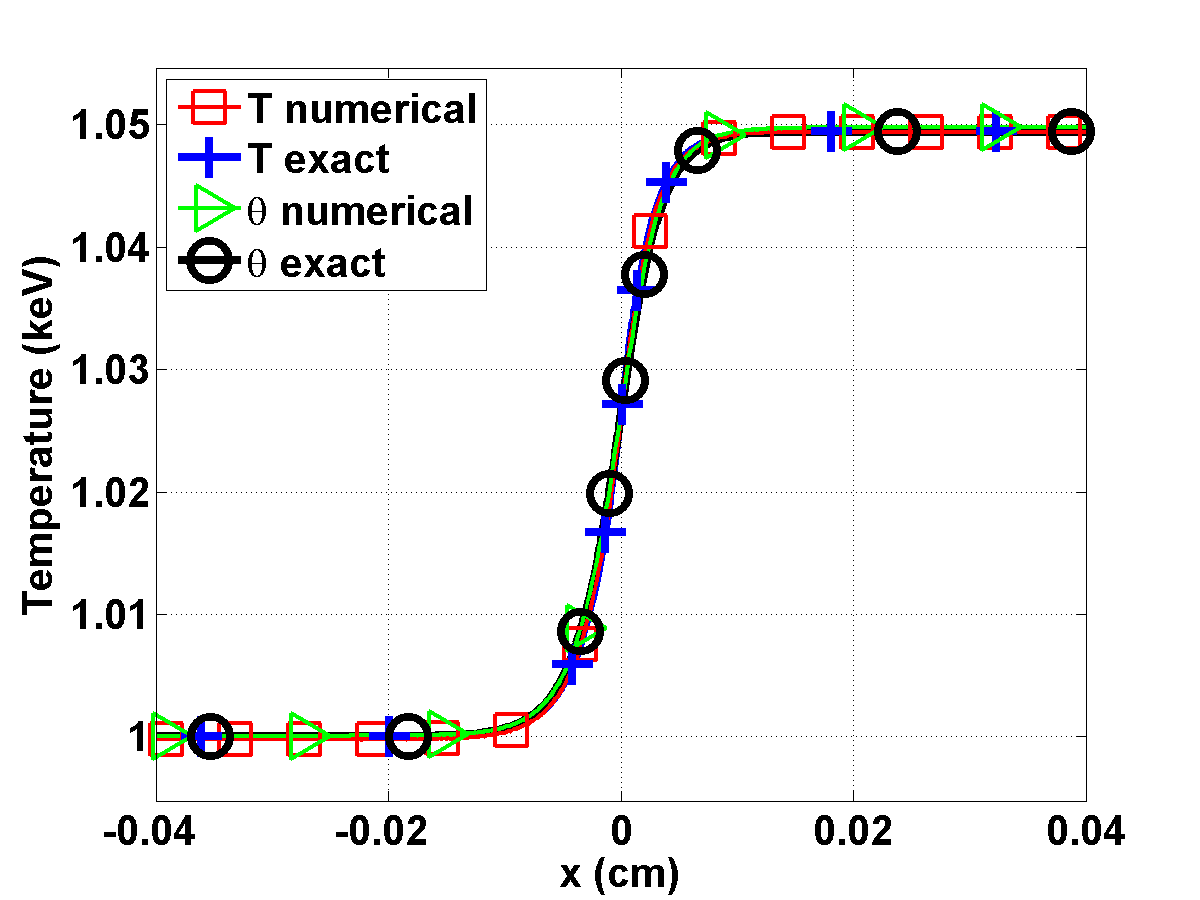
\includegraphics[width=0.4\textwidth]{figures_jcp/Mach_1p05_nel_500_temperature.png}
}
\subfigure[Material density]{
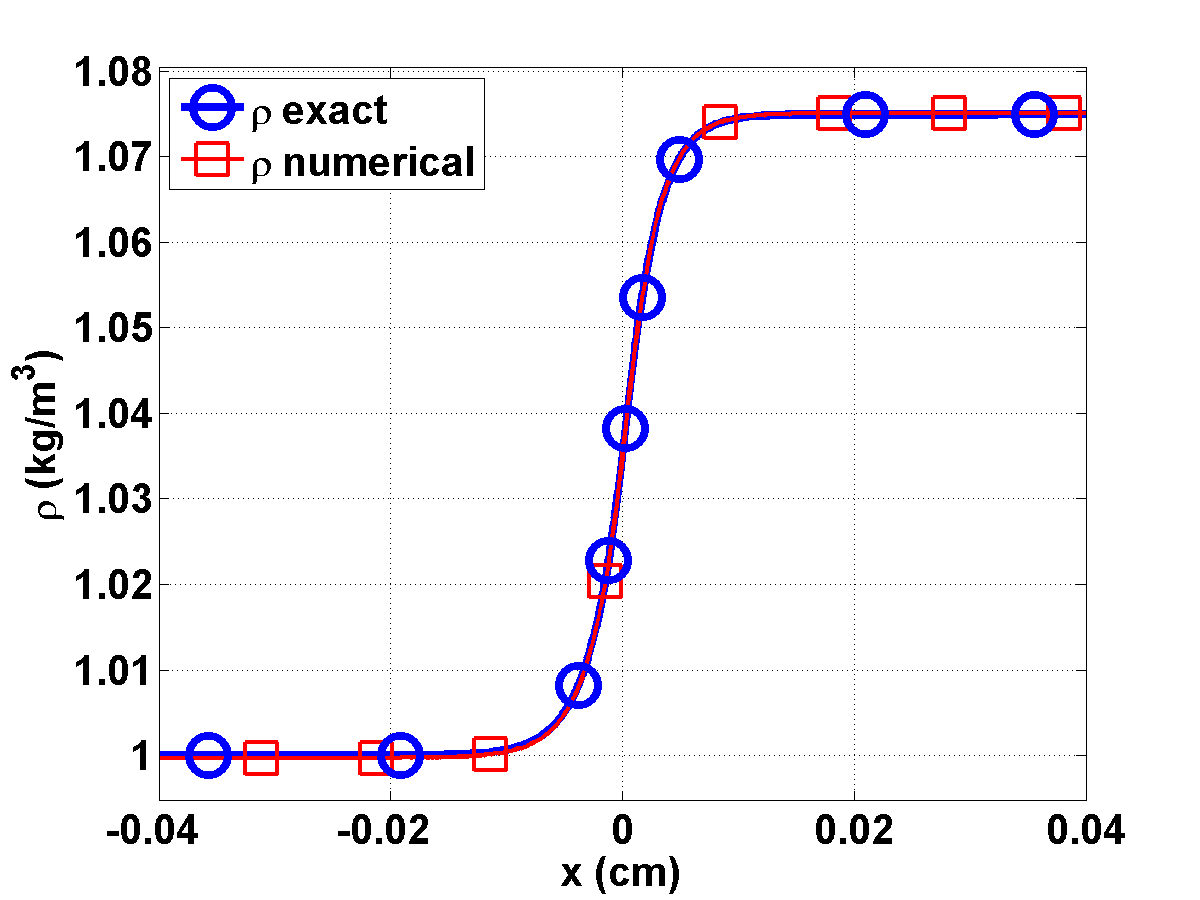
\includegraphics[width=0.4\textwidth]{figures_jcp/Mach_1p05_nel_500_density.png}
}
\\
\vspace{-3mm}
%
\subfigure[Viscosity coefficients]{
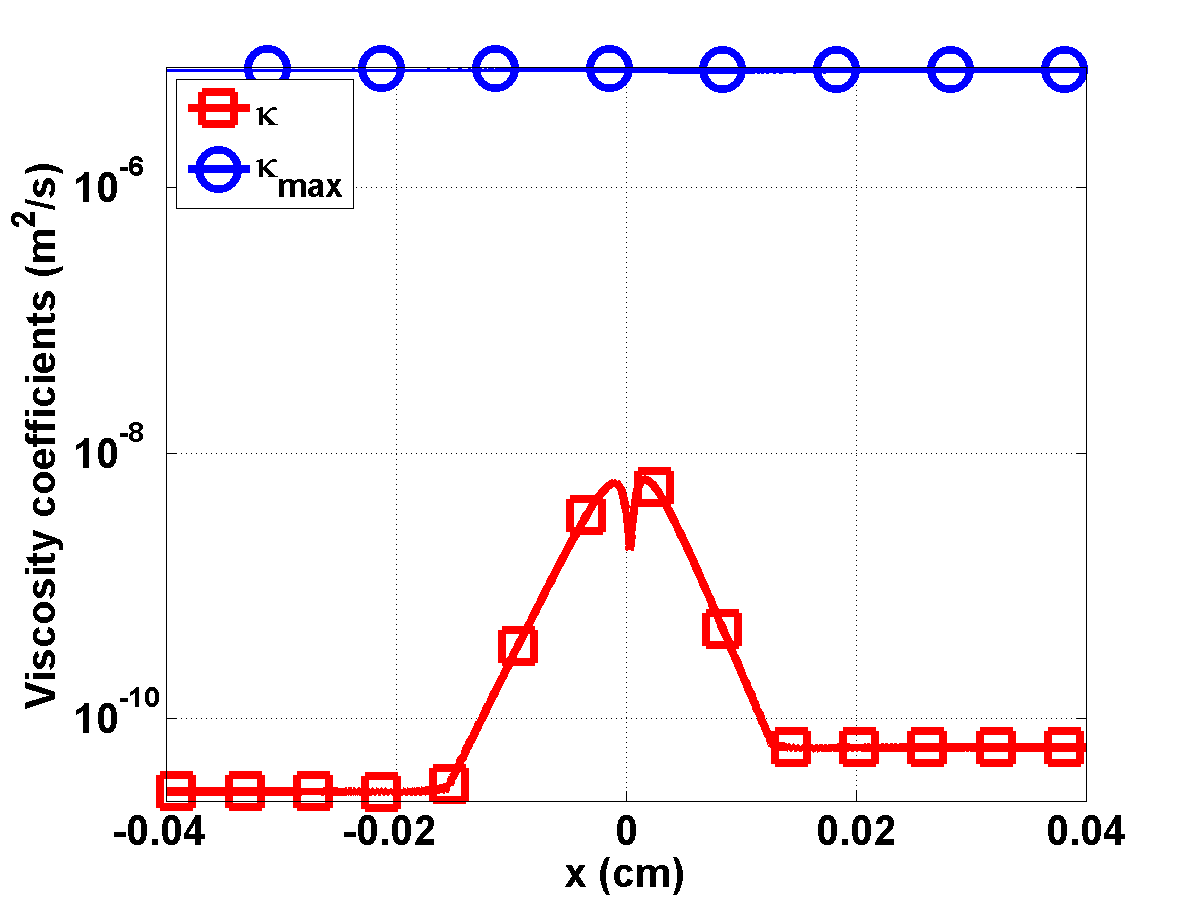
\includegraphics[width=0.4\textwidth]{figures_jcp/Mach_1p05_nel_500_viscosity.png}
}
\end{figure}

\end{frame}
%%%%%%%%%%%%%%%%%%%%%%%%%%%%%%%%%%%%%%%%%%%%%%%%%%%%%%%%%%%%%%%%%%%%


%%%%%%%%%%%%%%%%%%%%%%%%%%%%%%%%%%%%%%%%%%%%%%%%%%%%%%%%%%%%%%%%%%%%
\begin{frame}{Steady-state solution for Mach 2}
\setcounter{subfigure}{0}% Reset subfigure counter
\vspace{-4mm}

\begin{figure}[H]
\centering
\subfigure[Temperatures]{
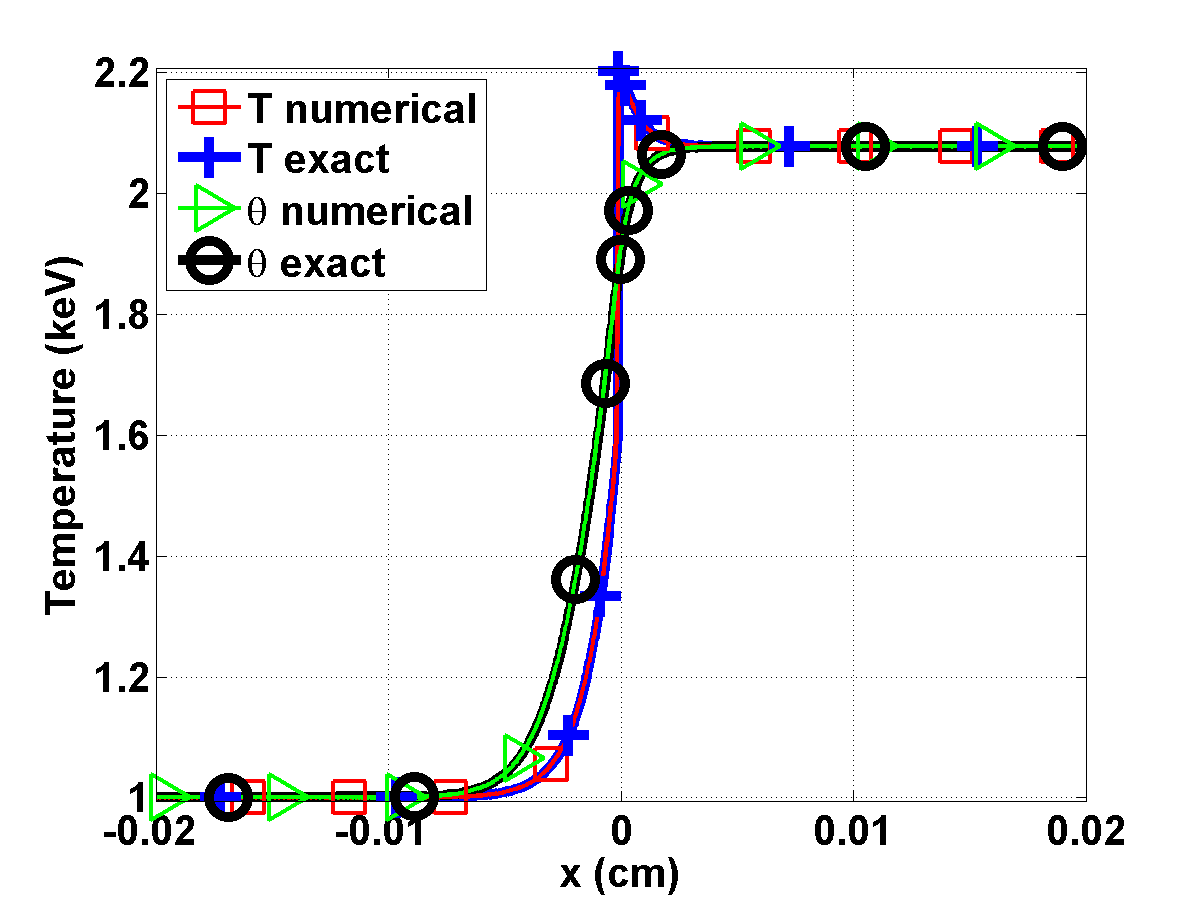
\includegraphics[width=0.4\textwidth]{figures_jcp/Mach_2_nel_2000_temperature.png}
}
\subfigure[Material density]{
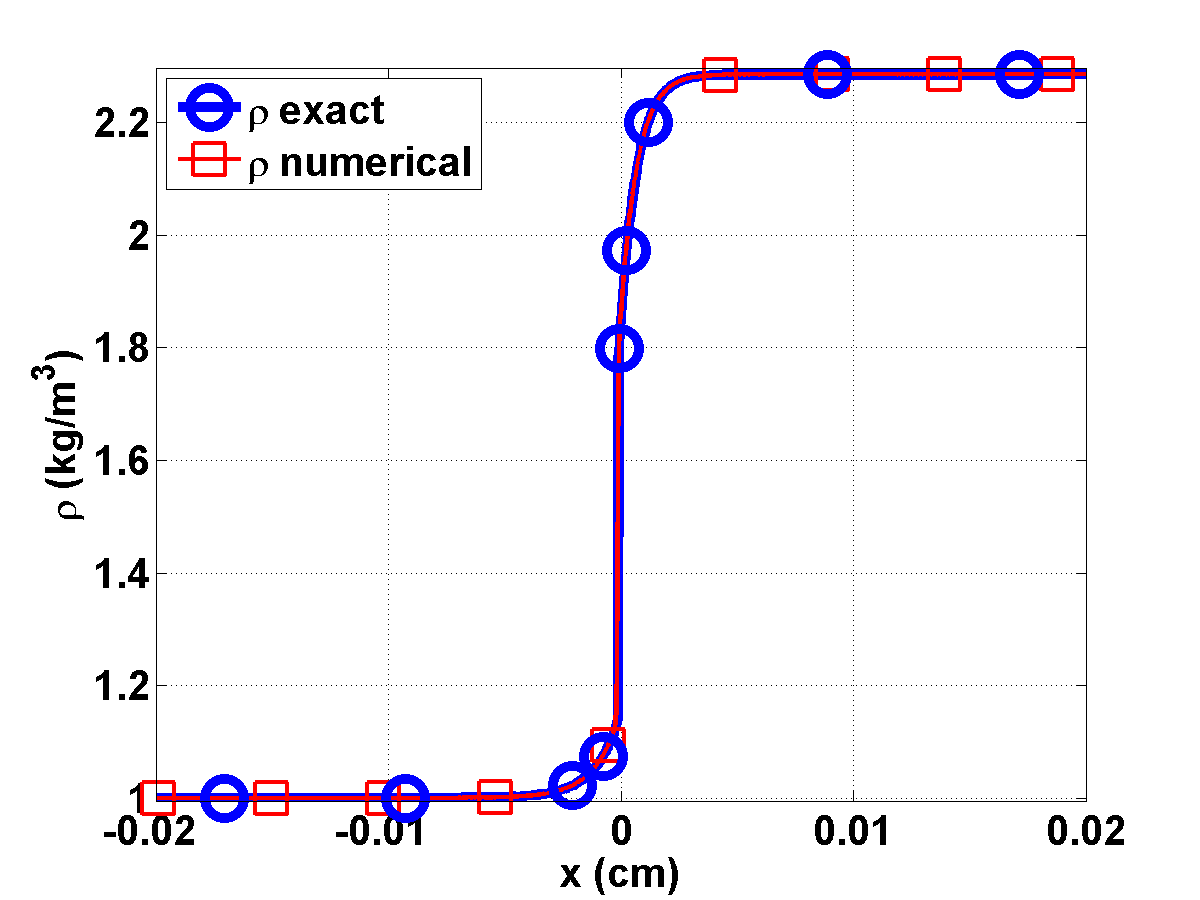
\includegraphics[width=0.4\textwidth]{figures_jcp/Mach_2_nel_2000_density.png}
}
\\
\vspace{-3mm}
%
\subfigure[Viscosity coefficients]{
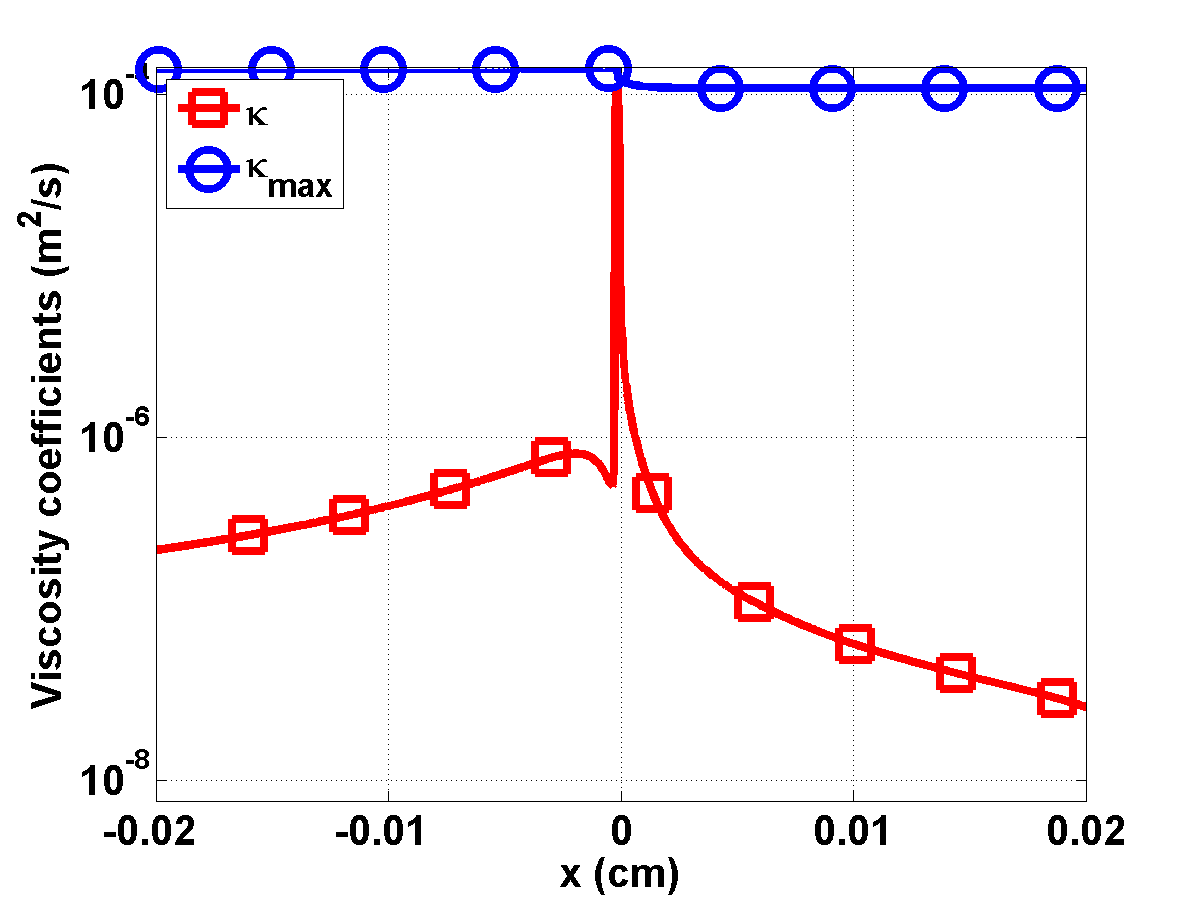
\includegraphics[width=0.4\textwidth]{figures_jcp/Mach_2_nel_2000_viscosity.png}
}
\end{figure}

\end{frame}
%%%%%%%%%%%%%%%%%%%%%%%%%%%%%%%%%%%%%%%%%%%%%%%%%%%%%%%%%%%%%%%%%%%%

%%%%%%%%%%%%%%%%%%%%%%%%%%%%%%%%%%%%%%%%%%%%%%%%%%%%%%%%%%%%%%%%%%%%
\begin{frame}{Steady-state solution for Mach 5}
\setcounter{subfigure}{0}% Reset subfigure counter
\vspace{-4mm}

\begin{figure}[H]
\centering
\subfigure[Temperatures]{
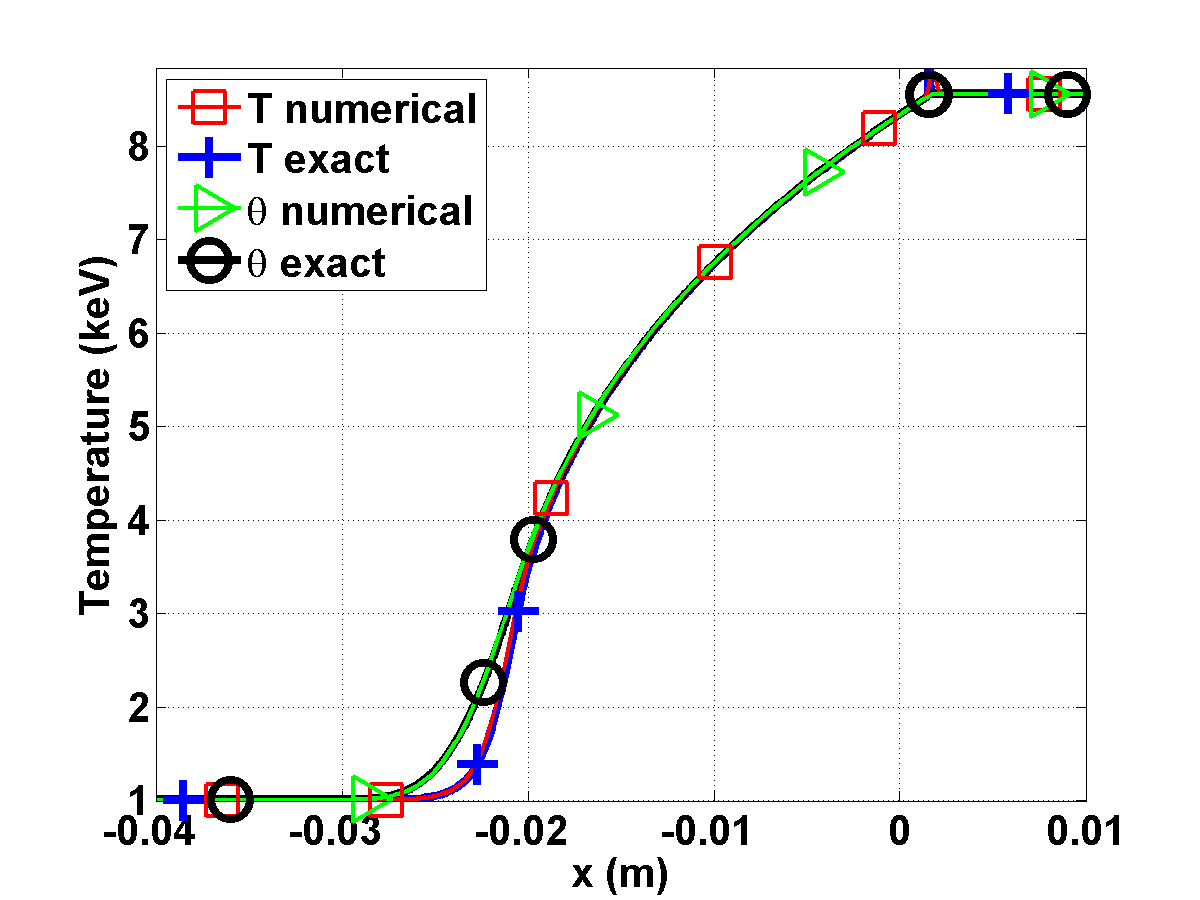
\includegraphics[width=0.4\textwidth]{figures_jcp/Mach_5_nel_1000_temperature.png}
}
\subfigure[Material density]{
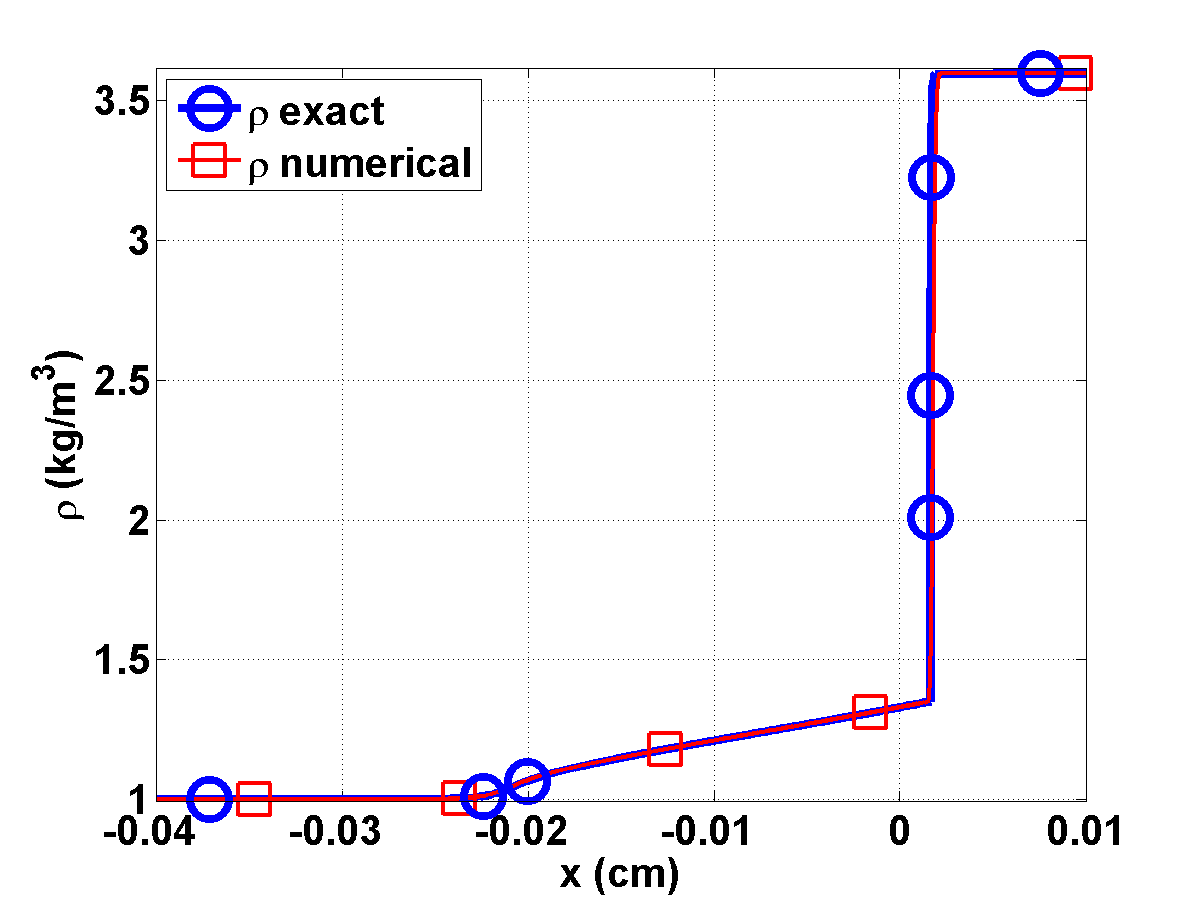
\includegraphics[width=0.4\textwidth]{figures_jcp/Mach_5_nel_2000_density.png}
}
\\
\vspace{-3mm}
%
\subfigure[Viscosity coefficients]{
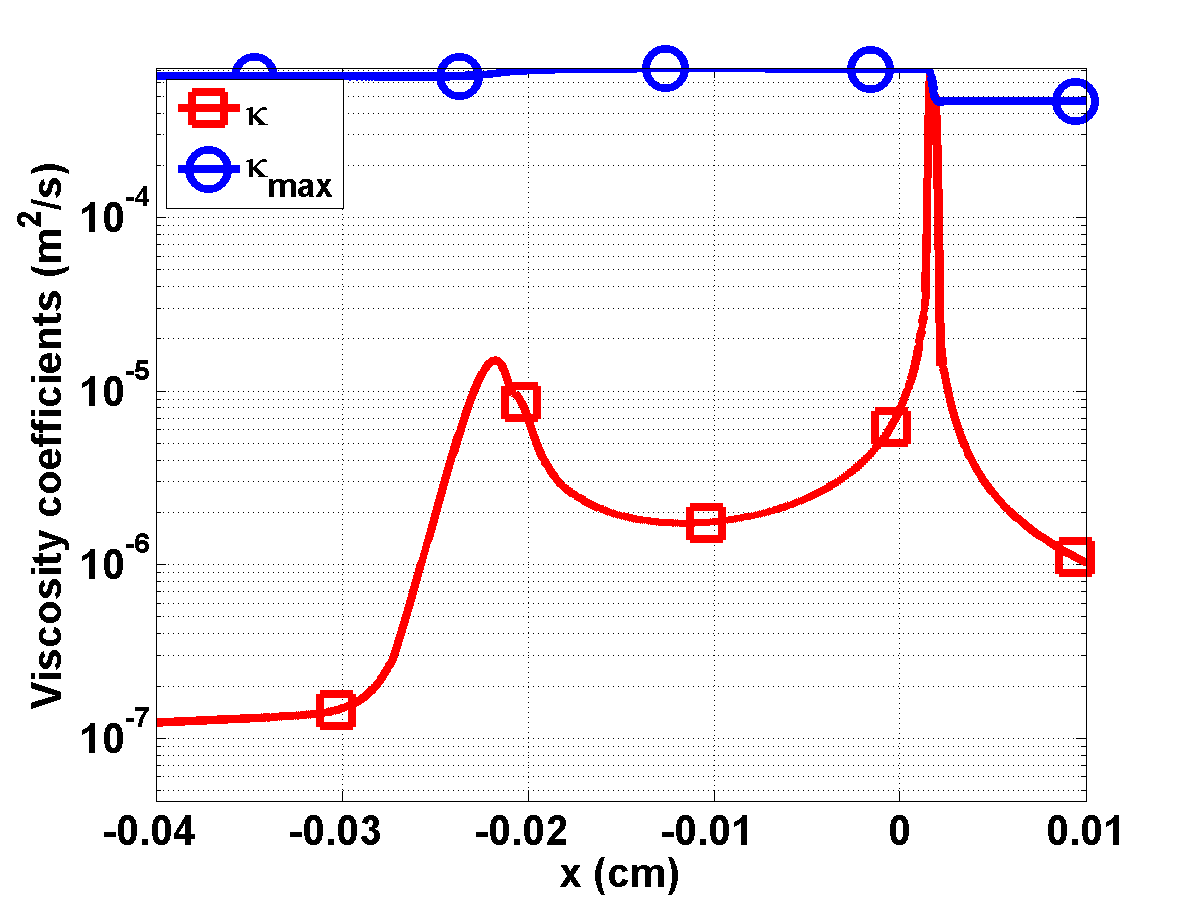
\includegraphics[width=0.4\textwidth]{figures_jcp/Mach_5_nel_2000_viscosity.png}
}
\subfigure[Zoom at the Z spike]{
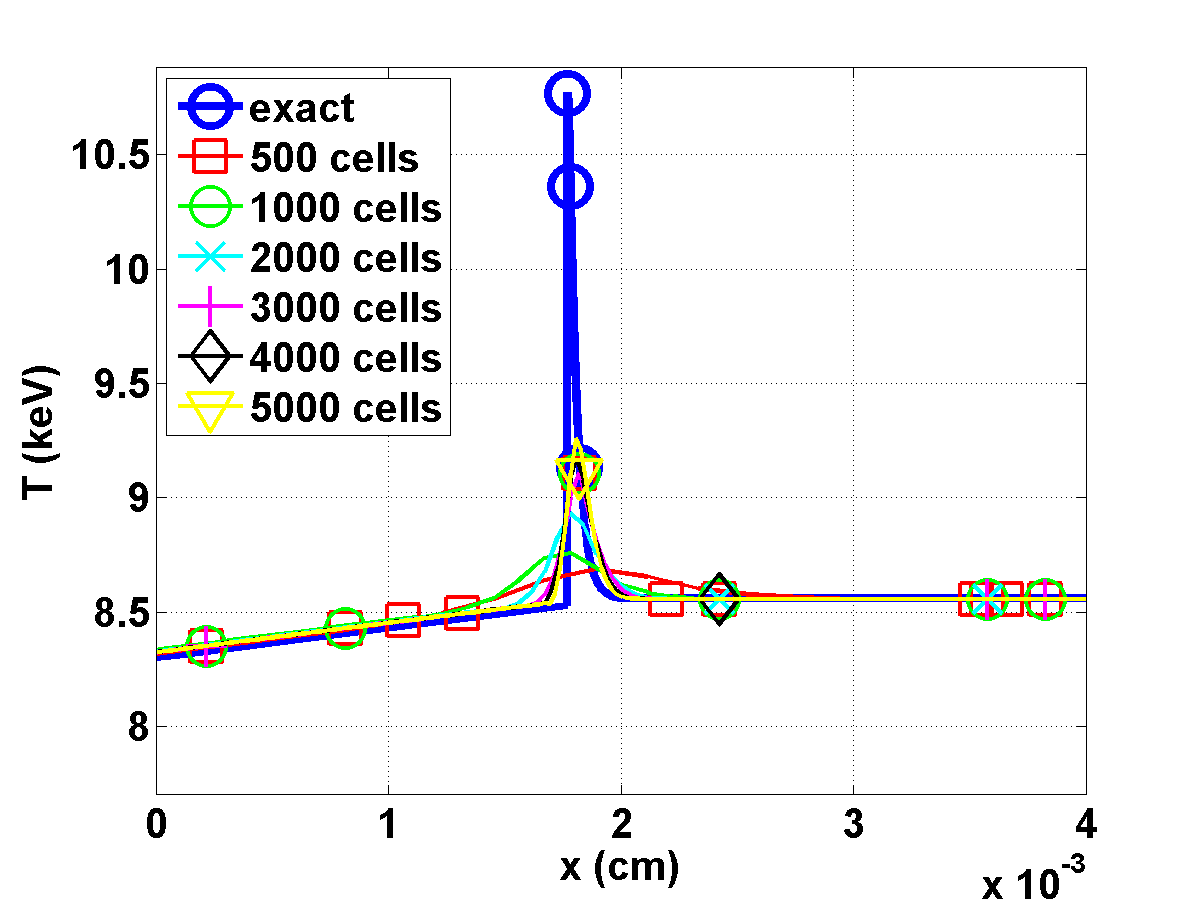
\includegraphics[width=0.4\textwidth]{figures_jcp/Mach_5_comparison.png}
}
\end{figure}


\end{frame}
%%%%%%%%%%%%%%%%%%%%%%%%%%%%%%%%%%%%%%%%%%%%%%%%%%%%%%%%%%%%%%%%%%%%

%%%%%%%%%%%%%%%%%%%%%%%%%%%%%%%%%%%%%%%%%%%%%%%%%%%%%%%%%%%%%%%%%%%%
\begin{frame}{Steady-state solution for Mach 50}
\setcounter{subfigure}{0}% Reset subfigure counter
\vspace{-4mm}

\begin{figure}[H]
\centering
\subfigure[Temperatures]{
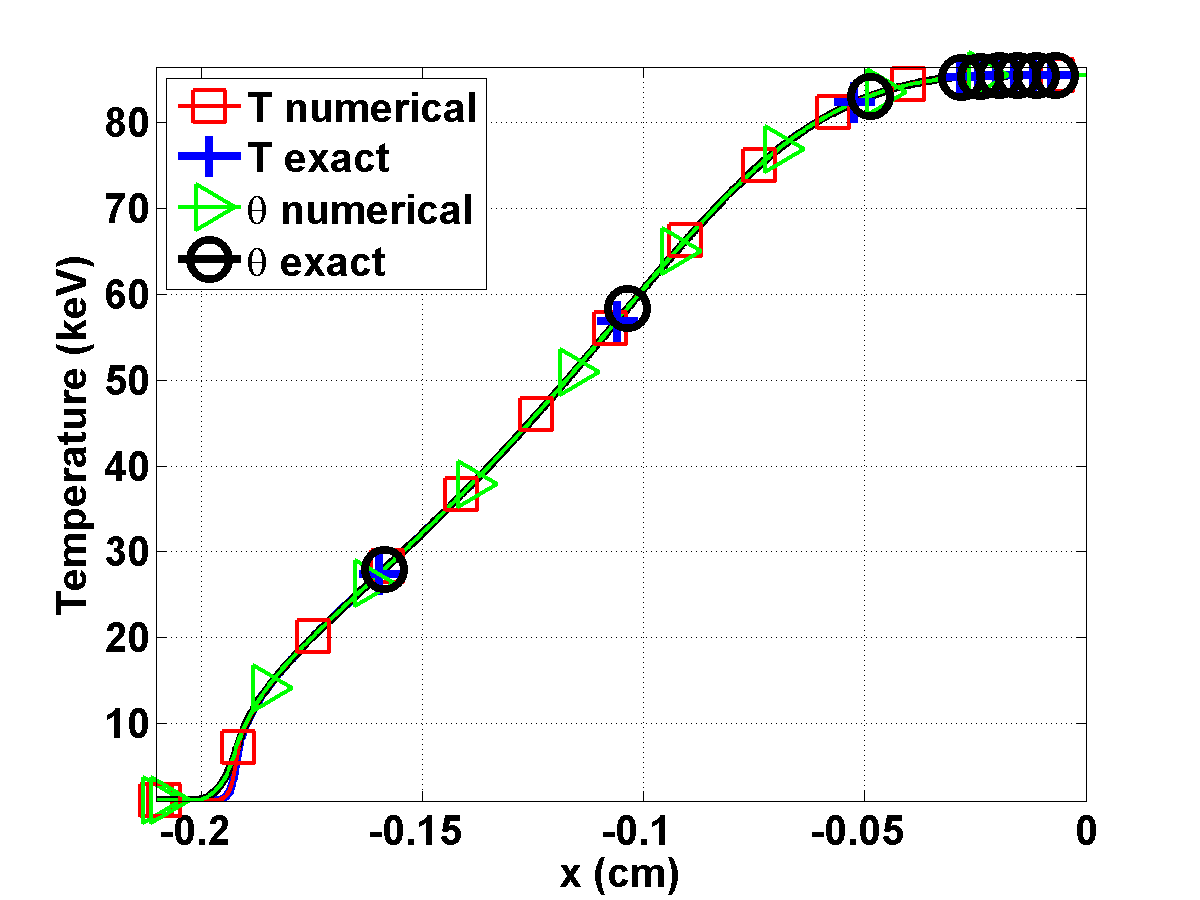
\includegraphics[width=0.4\textwidth]{figures_jcp/Mach_50_nel_1000_temperature.png}
}
\subfigure[Material density]{
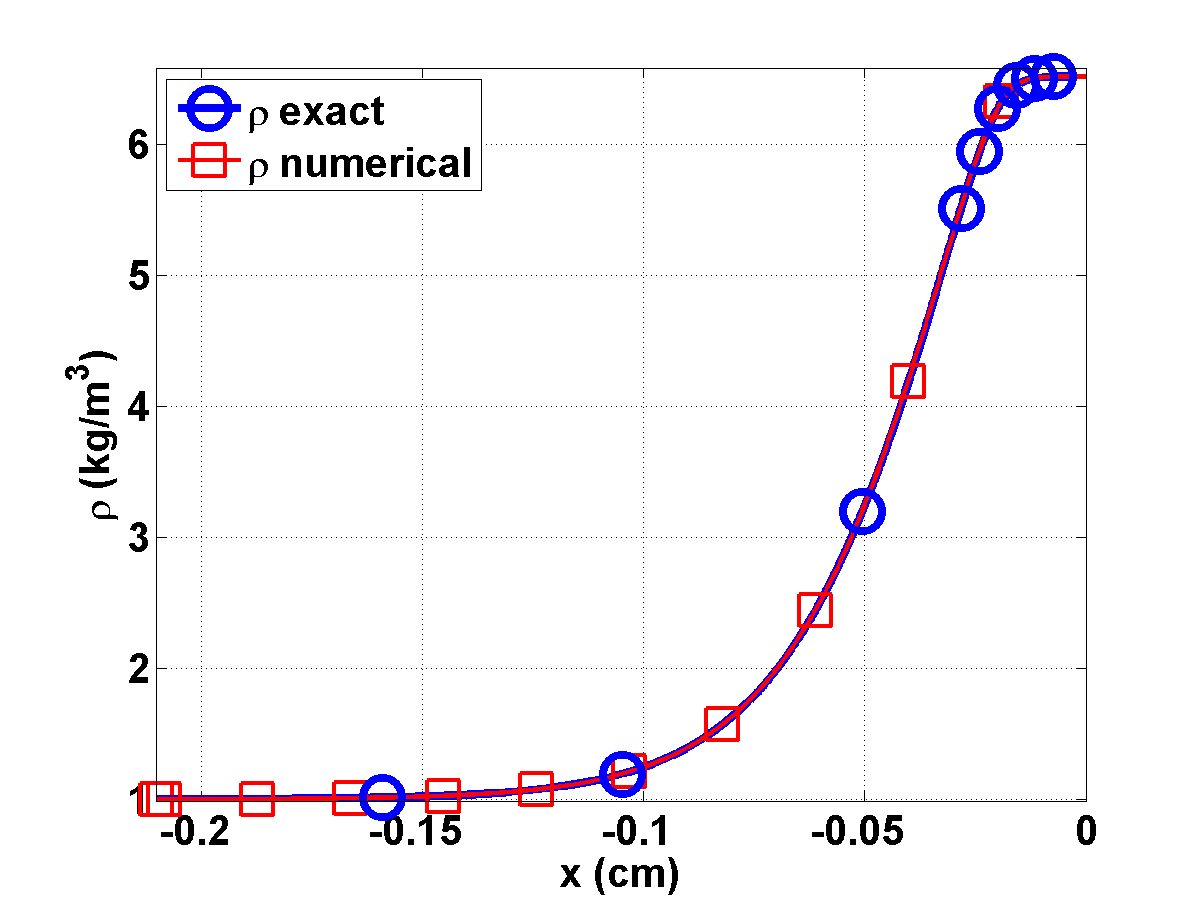
\includegraphics[width=0.4\textwidth]{figures_jcp/Mach_50_nel_1000_density.png}
}
\\
\vspace{-3mm}
%
\subfigure[Viscosity coefficients]{
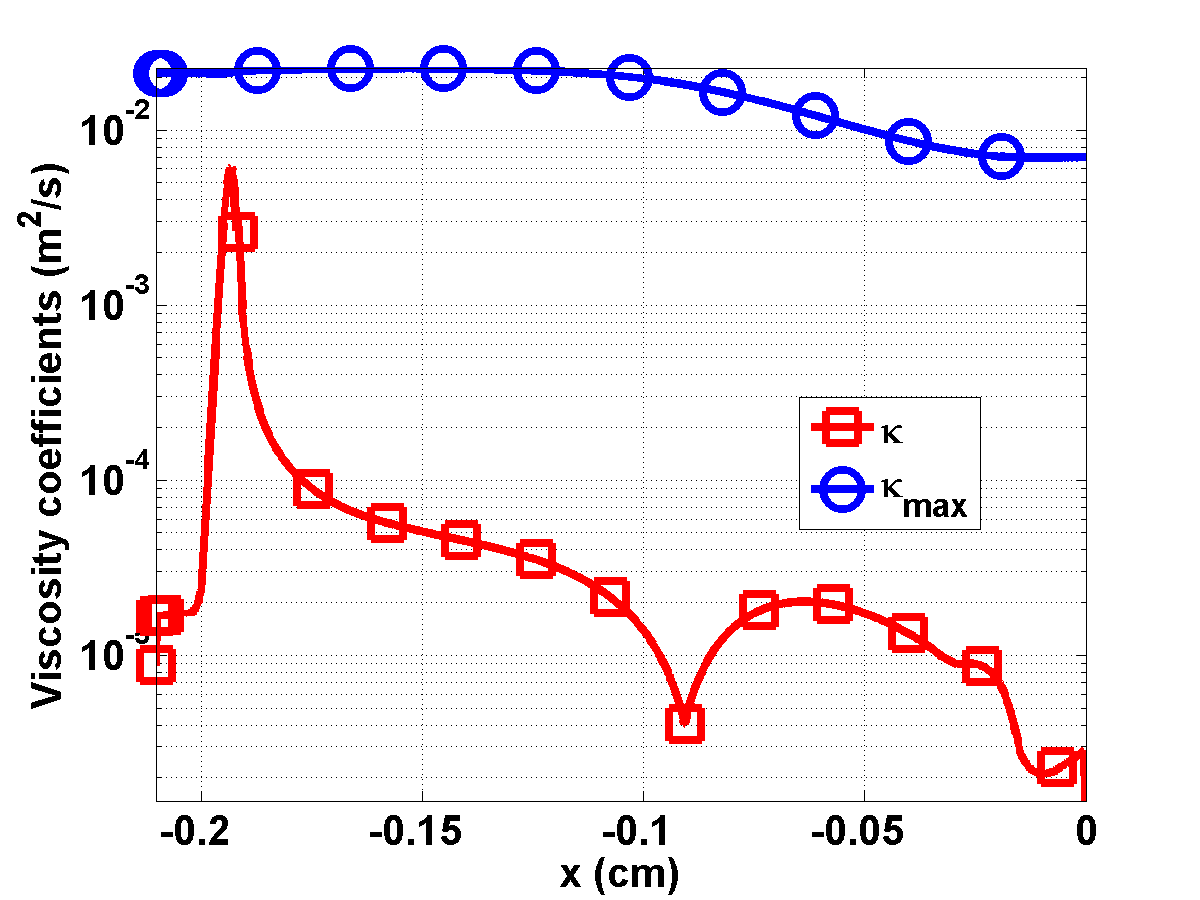
\includegraphics[width=0.4\textwidth]{figures_jcp/Mach_50_nel_1000_viscosity.png}
}
\end{figure}

\end{frame}
%%%%%%%%%%%%%%%%%%%%%%%%%%%%%%%%%%%%%%%%%%%%%%%%%%%%%%%%%%%%%%%%%%%%


%%%%%%%%%%%%%%%%%%%%%%%%%%%%%%%%%%%%%%%%%%%%%%%%%%%%%%%%%%%%%%%%%%%%
\subsubsection{Temperature-dependent opacities}
%%%%%%%%%%%%%%%%%%%%%%%%%%%%%%%%%%%%%%%%%%%%%%%%%%%%%%%%%%%%%%%%%%%%

%%%%%%%%%%%%%%%%%%%%%%%%%%%%%%%%%%%%%%%%%%%%%%%%%%%%%%%%%%%%%%%%%%%%
\begin{frame}{Steady-state solution for Mach 3:  \tcr{density}, 500 cells}

Now, results with temperature-dependent opacities:
\begin{figure}[H]
\centering
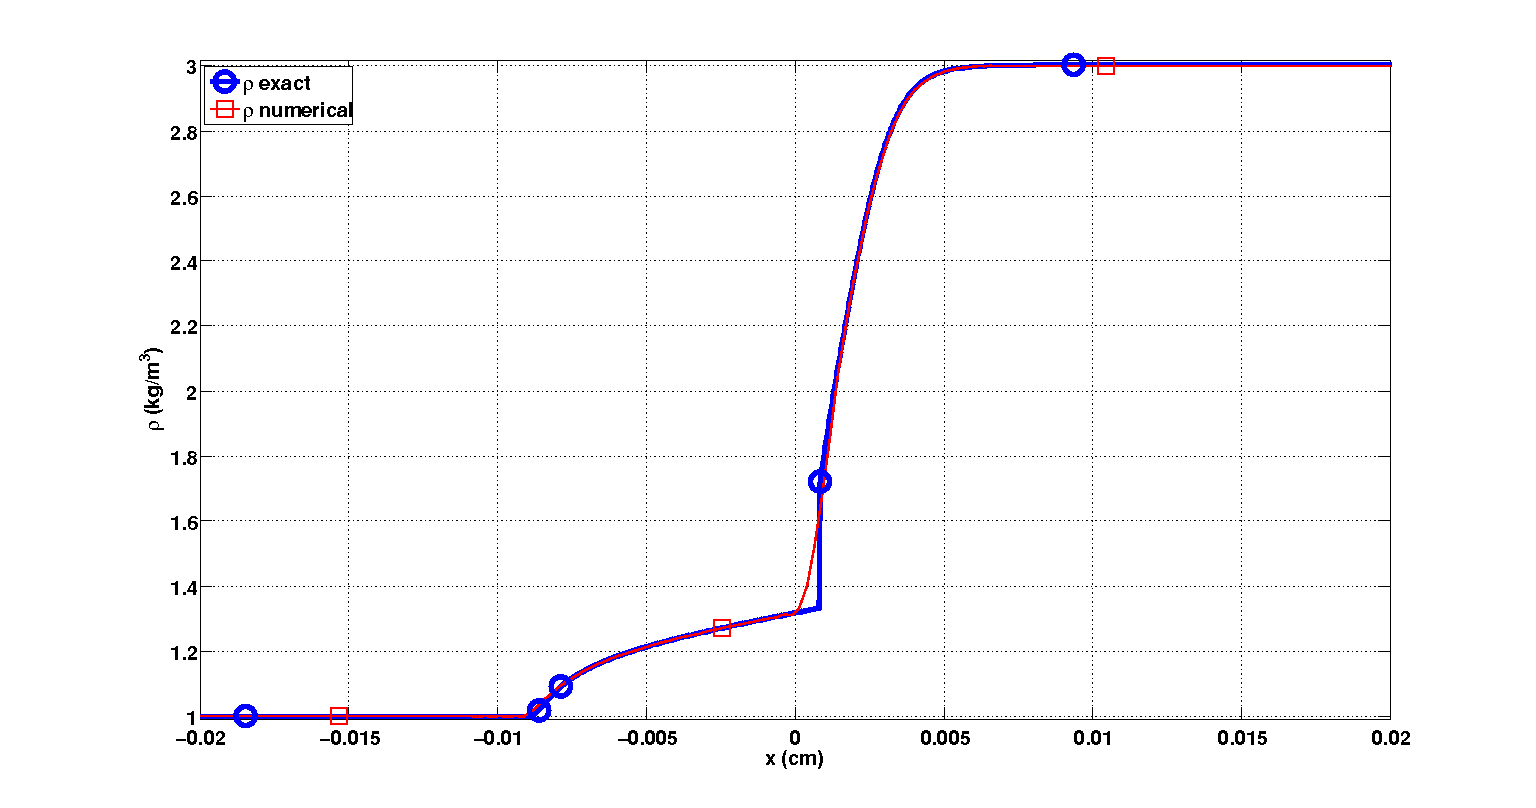
\includegraphics[width=0.99\textwidth]{figures_new_results/mach-3-temp-dpt-xs-density-500.png}
\end{figure}

\end{frame}
%%%%%%%%%%%%%%%%%%%%%%%%%%%%%%%%%%%%%%%%%%%%%%%%%%%%%%%%%%%%%%%%%%%%

%%%%%%%%%%%%%%%%%%%%%%%%%%%%%%%%%%%%%%%%%%%%%%%%%%%%%%%%%%%%%%%%%%%%
\begin{frame}{Steady-state solution for Mach 3:  \tcr{density}, 1000 cells}

\begin{figure}[H]
\centering
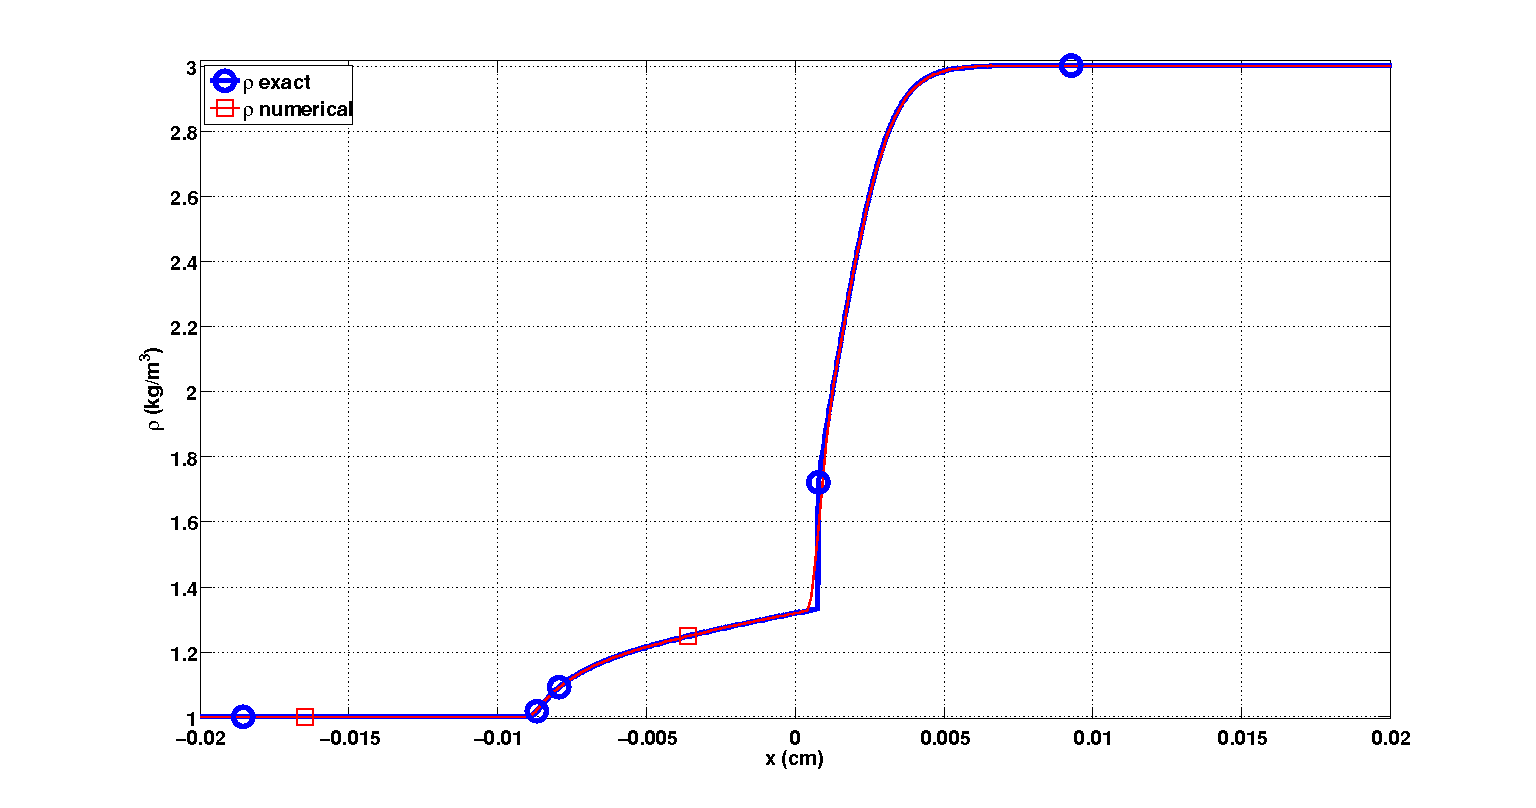
\includegraphics[width=0.99\textwidth]{figures_new_results/mach-3-temp-dpt-xs-density-1000.png}
\end{figure}

\end{frame}
%%%%%%%%%%%%%%%%%%%%%%%%%%%%%%%%%%%%%%%%%%%%%%%%%%%%%%%%%%%%%%%%%%%%

%%%%%%%%%%%%%%%%%%%%%%%%%%%%%%%%%%%%%%%%%%%%%%%%%%%%%%%%%%%%%%%%%%%%
\begin{frame}{Steady-state solution for Mach 3:  \tcr{density}, 2000 cells}

\begin{figure}[H]
\centering
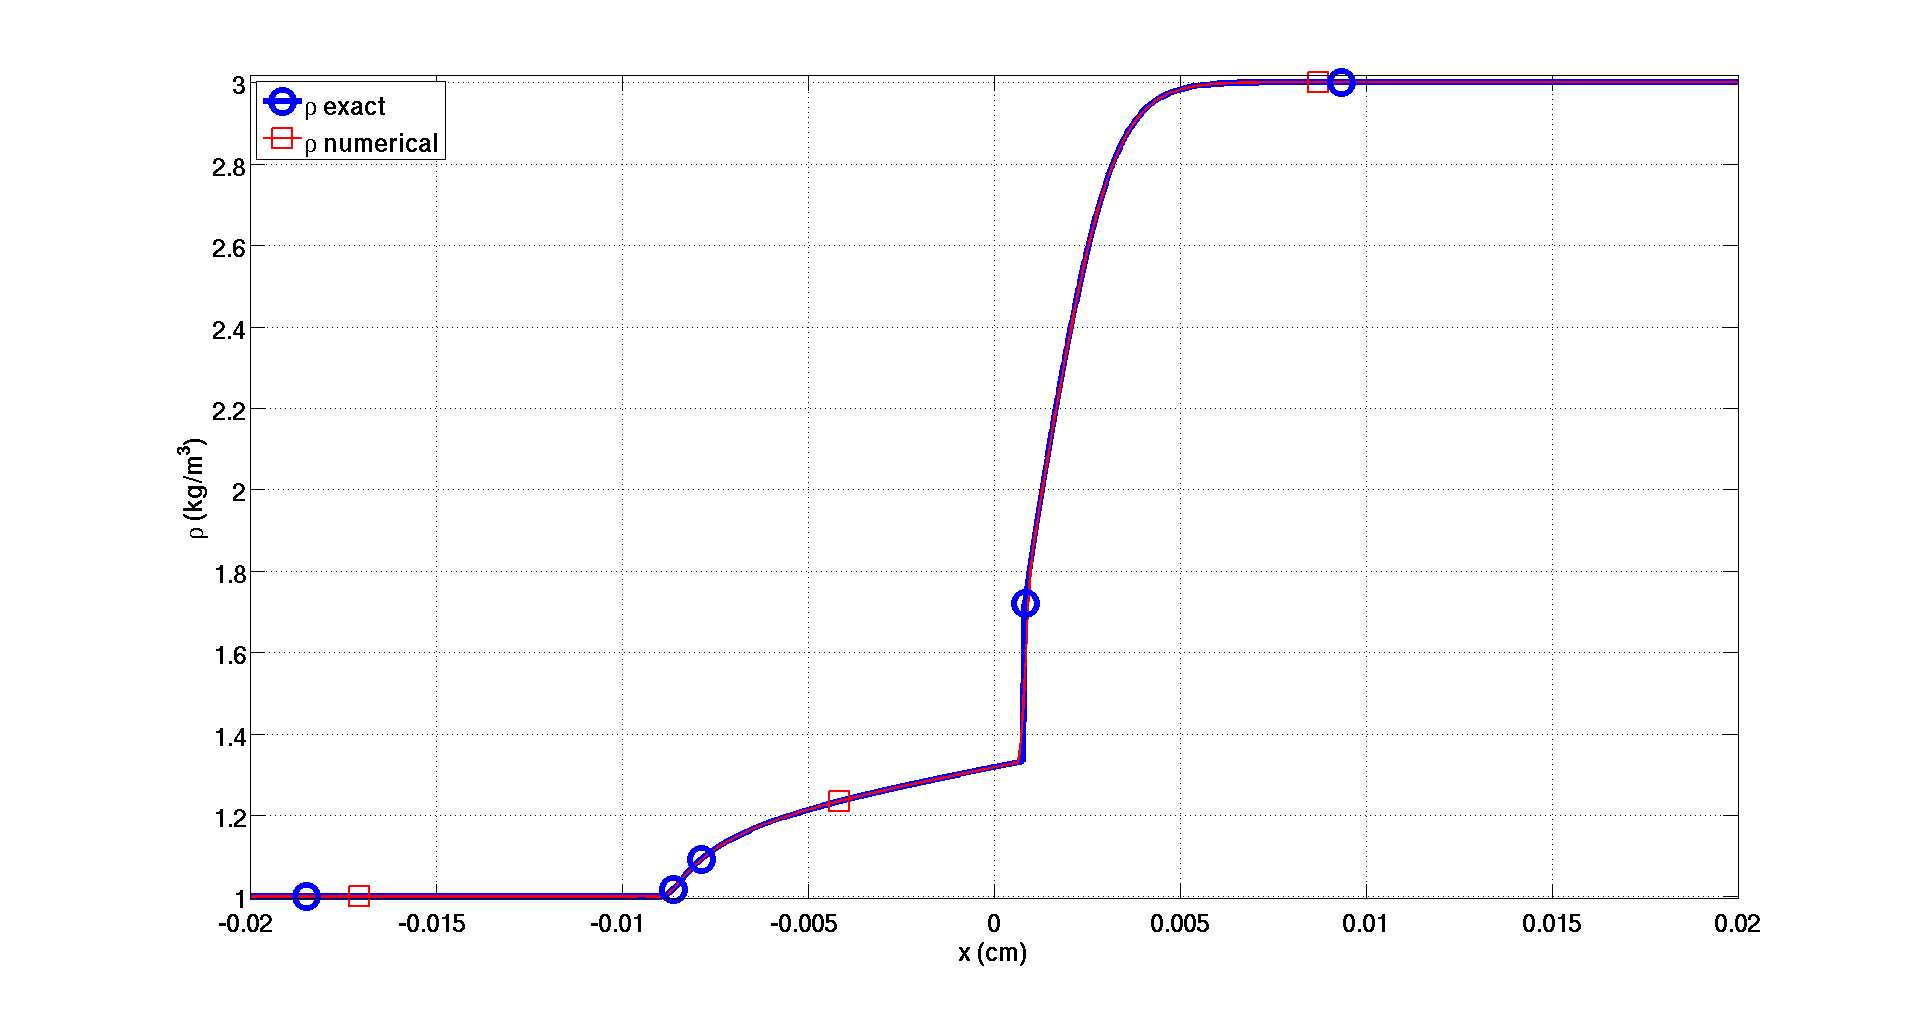
\includegraphics[width=0.99\textwidth]{figures_new_results/mach-3-temp-dpt-xs-density-2000.png}
\end{figure}

\end{frame}
%%%%%%%%%%%%%%%%%%%%%%%%%%%%%%%%%%%%%%%%%%%%%%%%%%%%%%%%%%%%%%%%%%%%

%%%%%%%%%%%%%%%%%%%%%%%%%%%%%%%%%%%%%%%%%%%%%%%%%%%%%%%%%%%%%%%%%%%%
\begin{frame}{Steady-state solution for Mach 3:  \tcr{temperature}, 500 cells}

\begin{figure}[H]
\centering
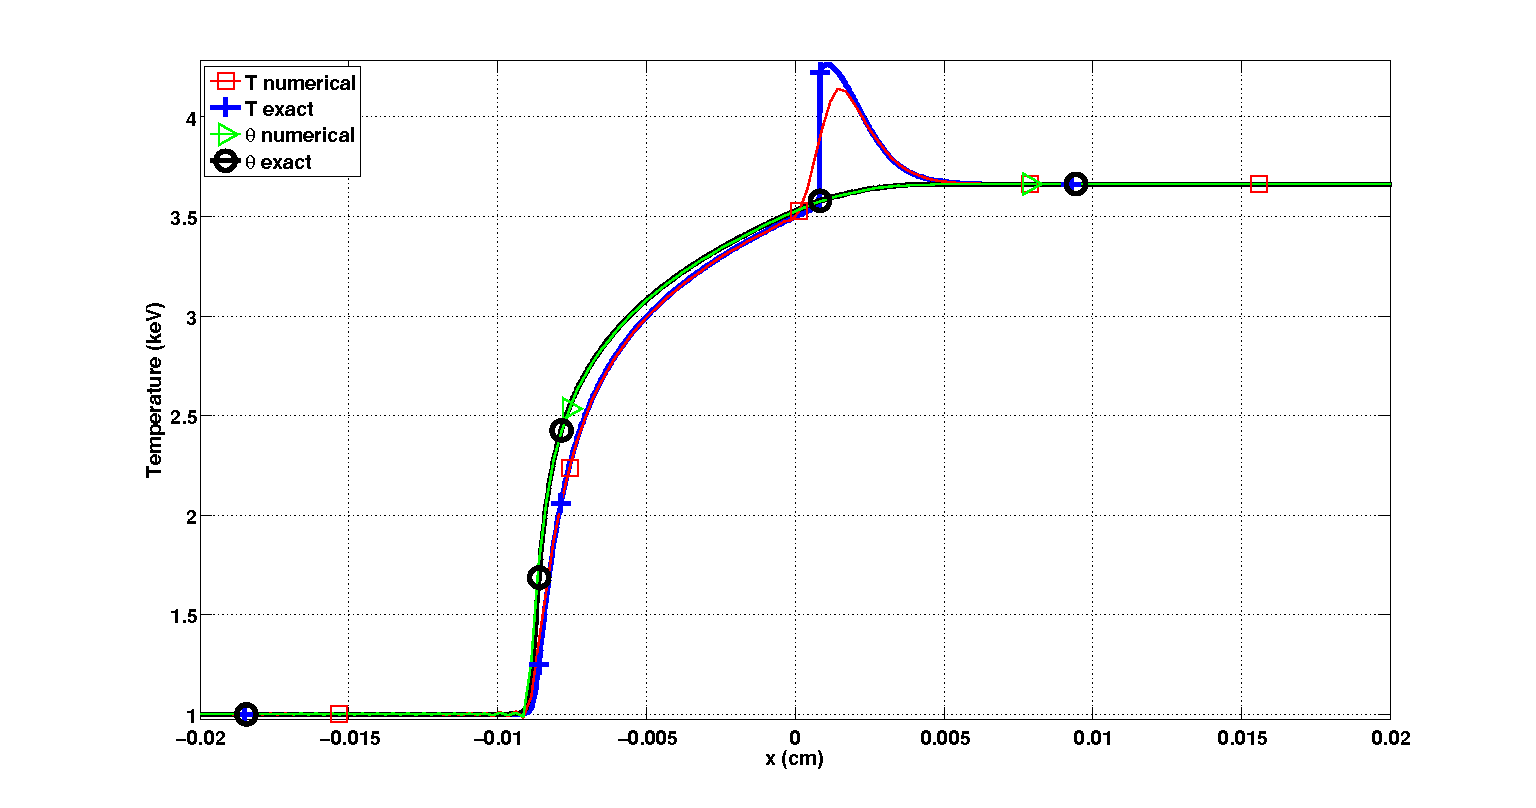
\includegraphics[width=0.99\textwidth]{figures_new_results/mach-3-temp-dpt-xs-temperature-500.png}
\end{figure}

\end{frame}
%%%%%%%%%%%%%%%%%%%%%%%%%%%%%%%%%%%%%%%%%%%%%%%%%%%%%%%%%%%%%%%%%%%%

%%%%%%%%%%%%%%%%%%%%%%%%%%%%%%%%%%%%%%%%%%%%%%%%%%%%%%%%%%%%%%%%%%%%
\begin{frame}{Steady-state solution for Mach 3:  \tcr{temperature}, 1000 cells}

\begin{figure}[H]
\centering
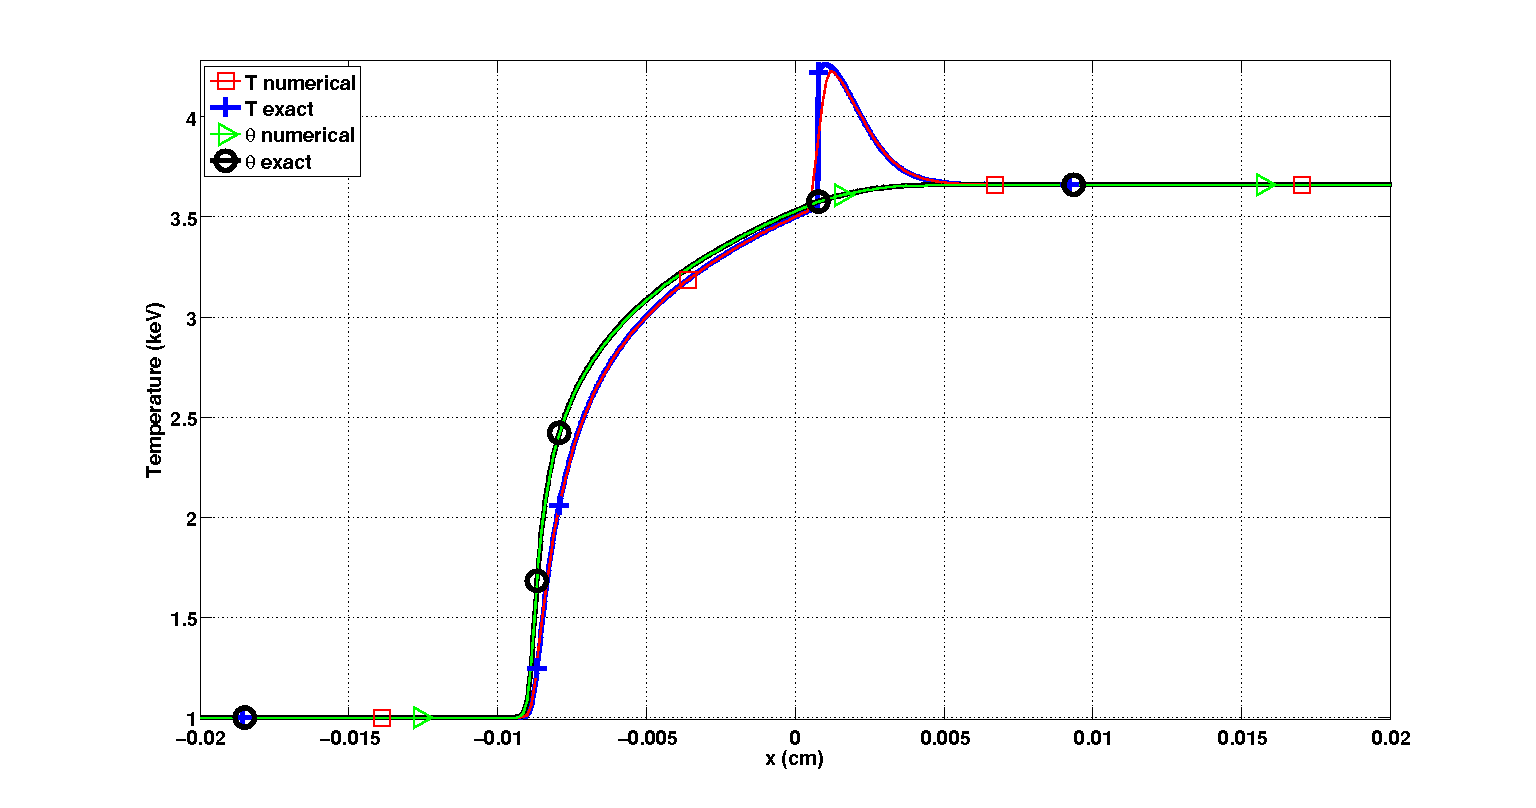
\includegraphics[width=0.99\textwidth]{figures_new_results/mach-3-temp-dpt-xs-temperature-1000.png}
\end{figure}

\end{frame}
%%%%%%%%%%%%%%%%%%%%%%%%%%%%%%%%%%%%%%%%%%%%%%%%%%%%%%%%%%%%%%%%%%%%

%%%%%%%%%%%%%%%%%%%%%%%%%%%%%%%%%%%%%%%%%%%%%%%%%%%%%%%%%%%%%%%%%%%%
\begin{frame}{Steady-state solution for Mach 3:  \tcr{temperature}, 2000 cells}

\begin{figure}[H]
\centering
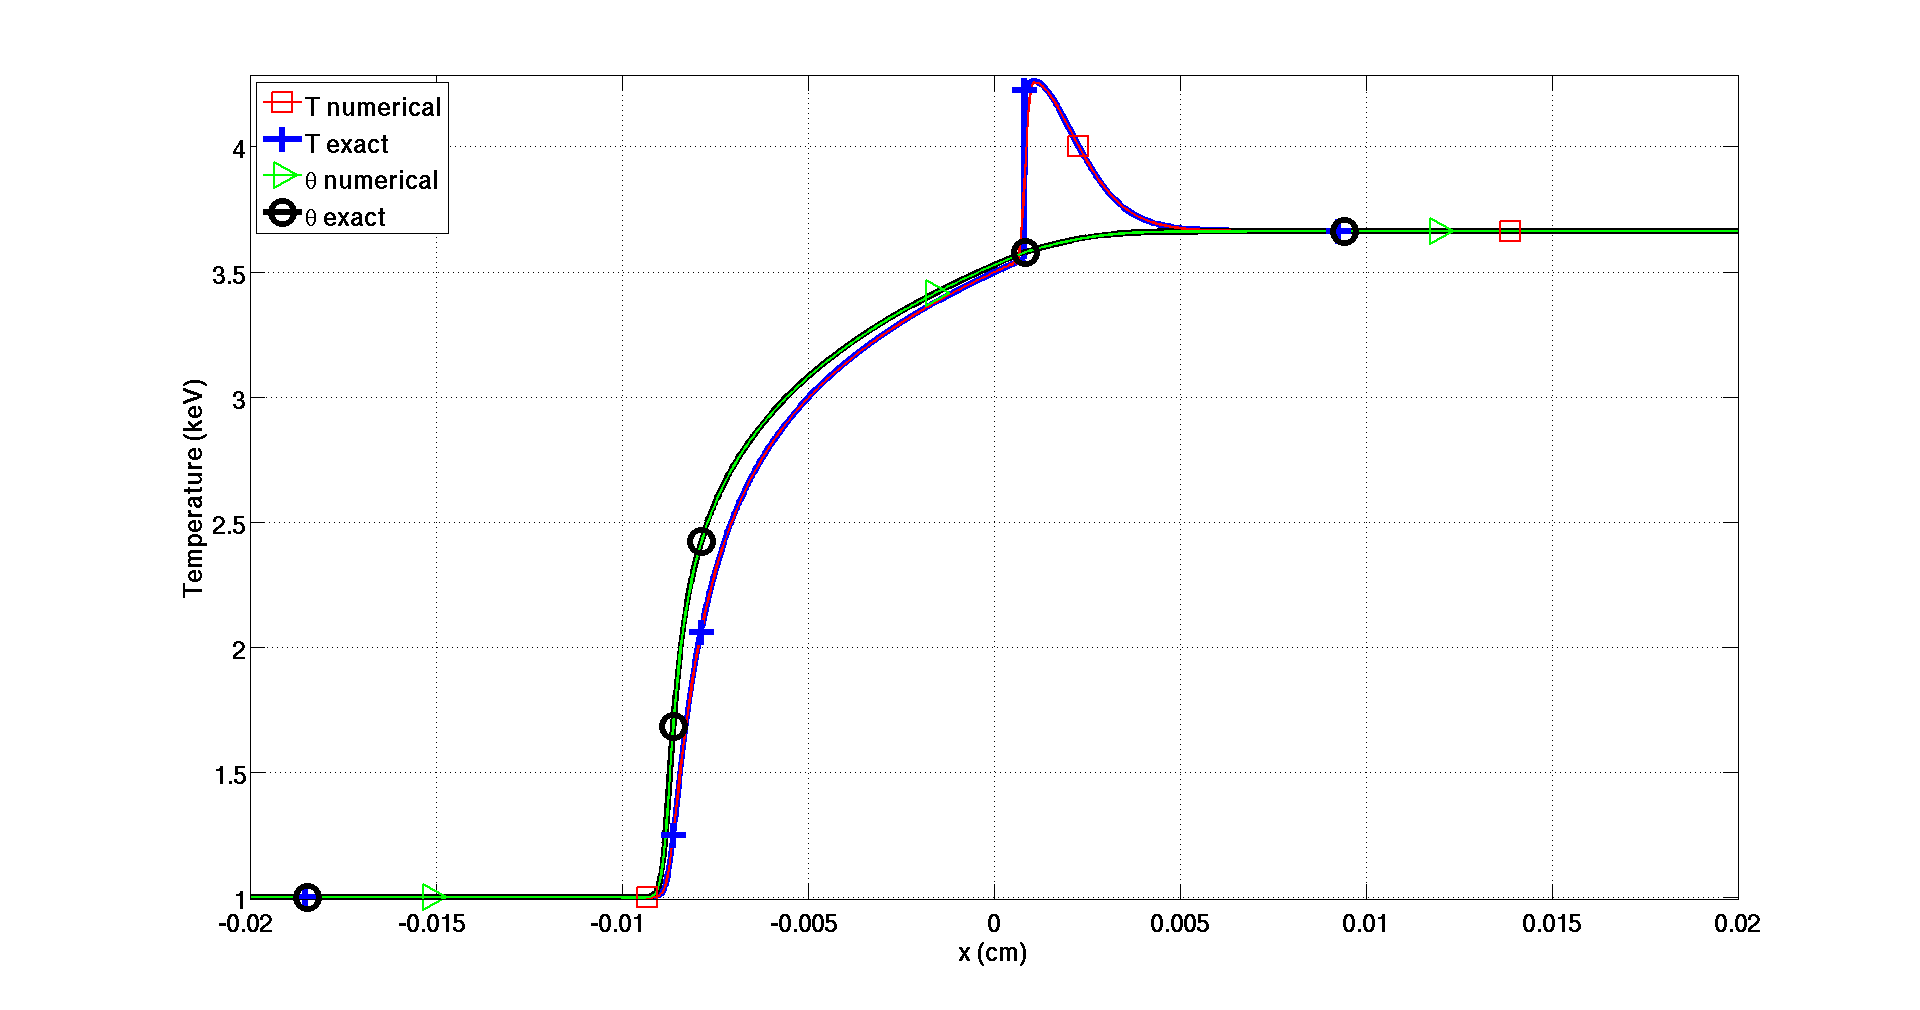
\includegraphics[width=0.99\textwidth]{figures_new_results/mach-3-temp-dpt-xs-temperature-2000.png}
\end{figure}

\end{frame}
%%%%%%%%%%%%%%%%%%%%%%%%%%%%%%%%%%%%%%%%%%%%%%%%%%%%%%%%%%%%%%%%%%%%

%%%%%%%%%%%%%%%%%%%%%%%%%%%%%%%%%%%%%%%%%%%%%%%%%%%%%%%%%%%%%%%%%%%%
\begin{frame}{Steady-state solution for Mach 3:  \tcr{viscosity}, 500 cells}

\begin{figure}[H]
\centering
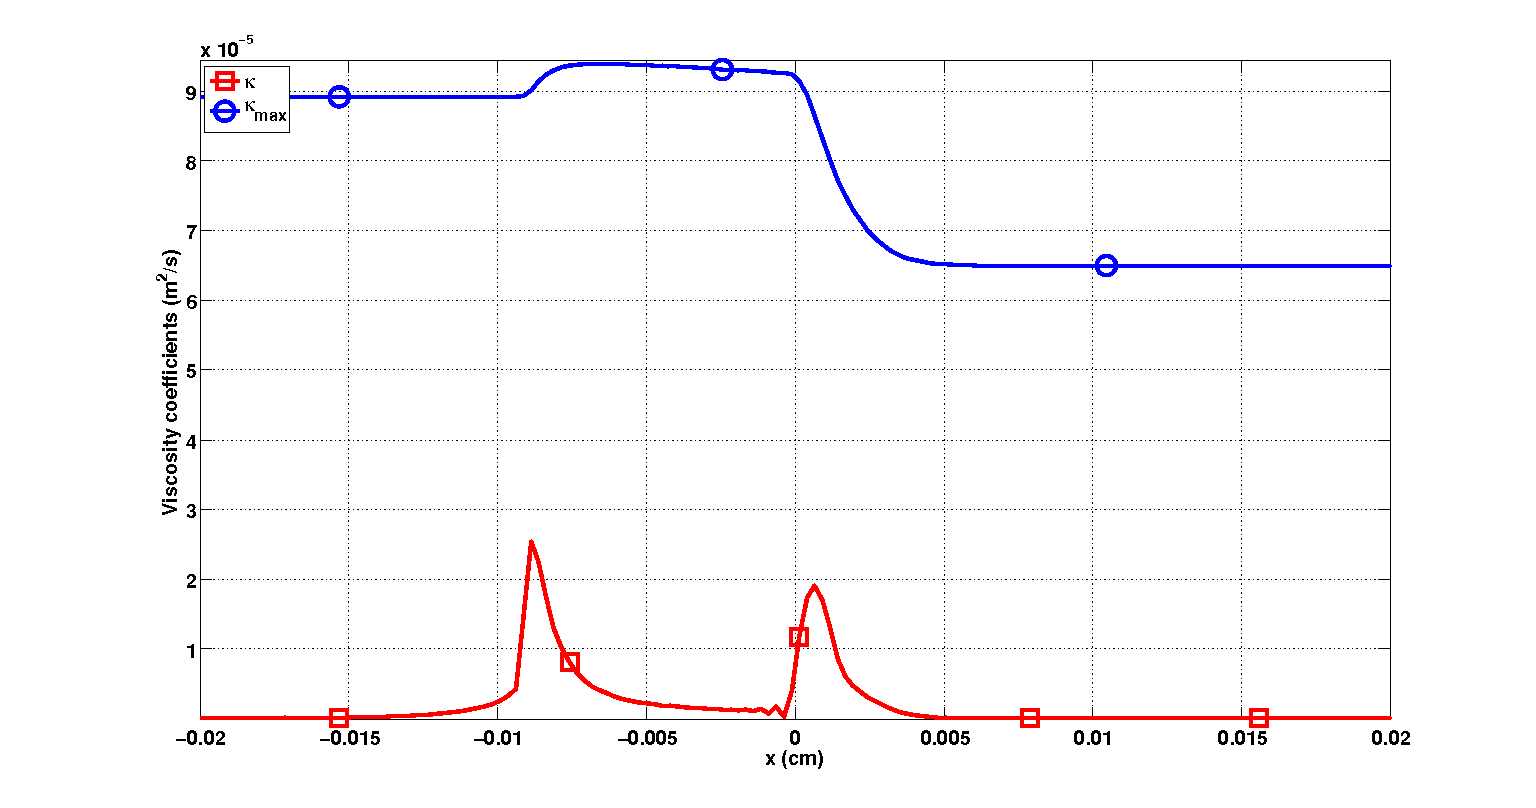
\includegraphics[width=0.99\textwidth]{figures_new_results/mach-3-temp-dpt-xs-viscosity-500.png}
\end{figure}

\end{frame}
%%%%%%%%%%%%%%%%%%%%%%%%%%%%%%%%%%%%%%%%%%%%%%%%%%%%%%%%%%%%%%%%%%%%

%%%%%%%%%%%%%%%%%%%%%%%%%%%%%%%%%%%%%%%%%%%%%%%%%%%%%%%%%%%%%%%%%%%%
\begin{frame}{Steady-state solution for Mach 3:  \tcr{viscosity}, 1000 cells}

\begin{figure}[H]
\centering
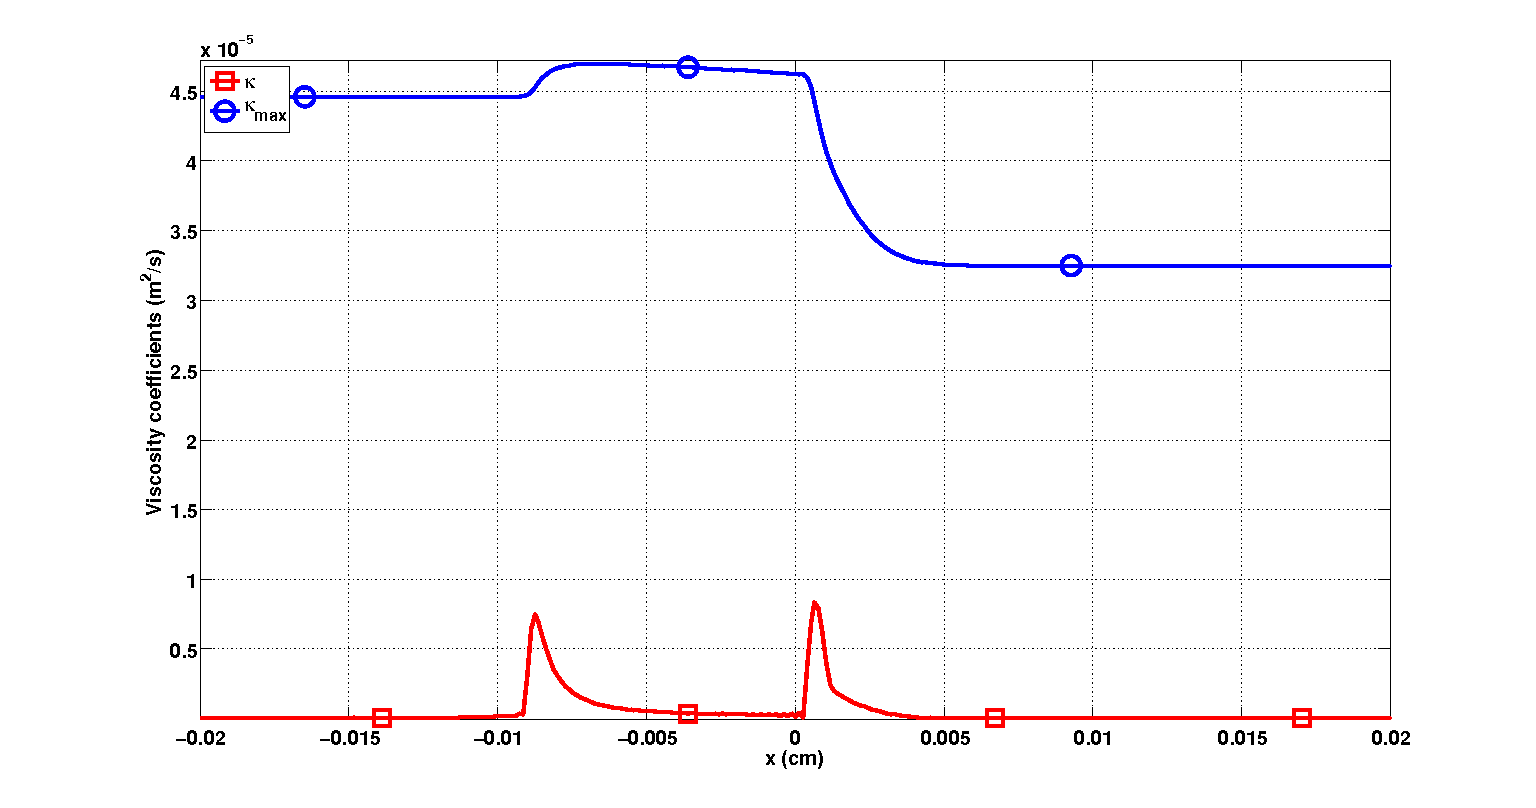
\includegraphics[width=0.99\textwidth]{figures_new_results/mach-3-temp-dpt-xs-viscosity-1000.png}
\end{figure}

\end{frame}
%%%%%%%%%%%%%%%%%%%%%%%%%%%%%%%%%%%%%%%%%%%%%%%%%%%%%%%%%%%%%%%%%%%%

%%%%%%%%%%%%%%%%%%%%%%%%%%%%%%%%%%%%%%%%%%%%%%%%%%%%%%%%%%%%%%%%%%%%
\begin{frame}{Steady-state solution for Mach 3:  \tcr{viscosity}, 2000 cells}

\begin{figure}[H]
\centering
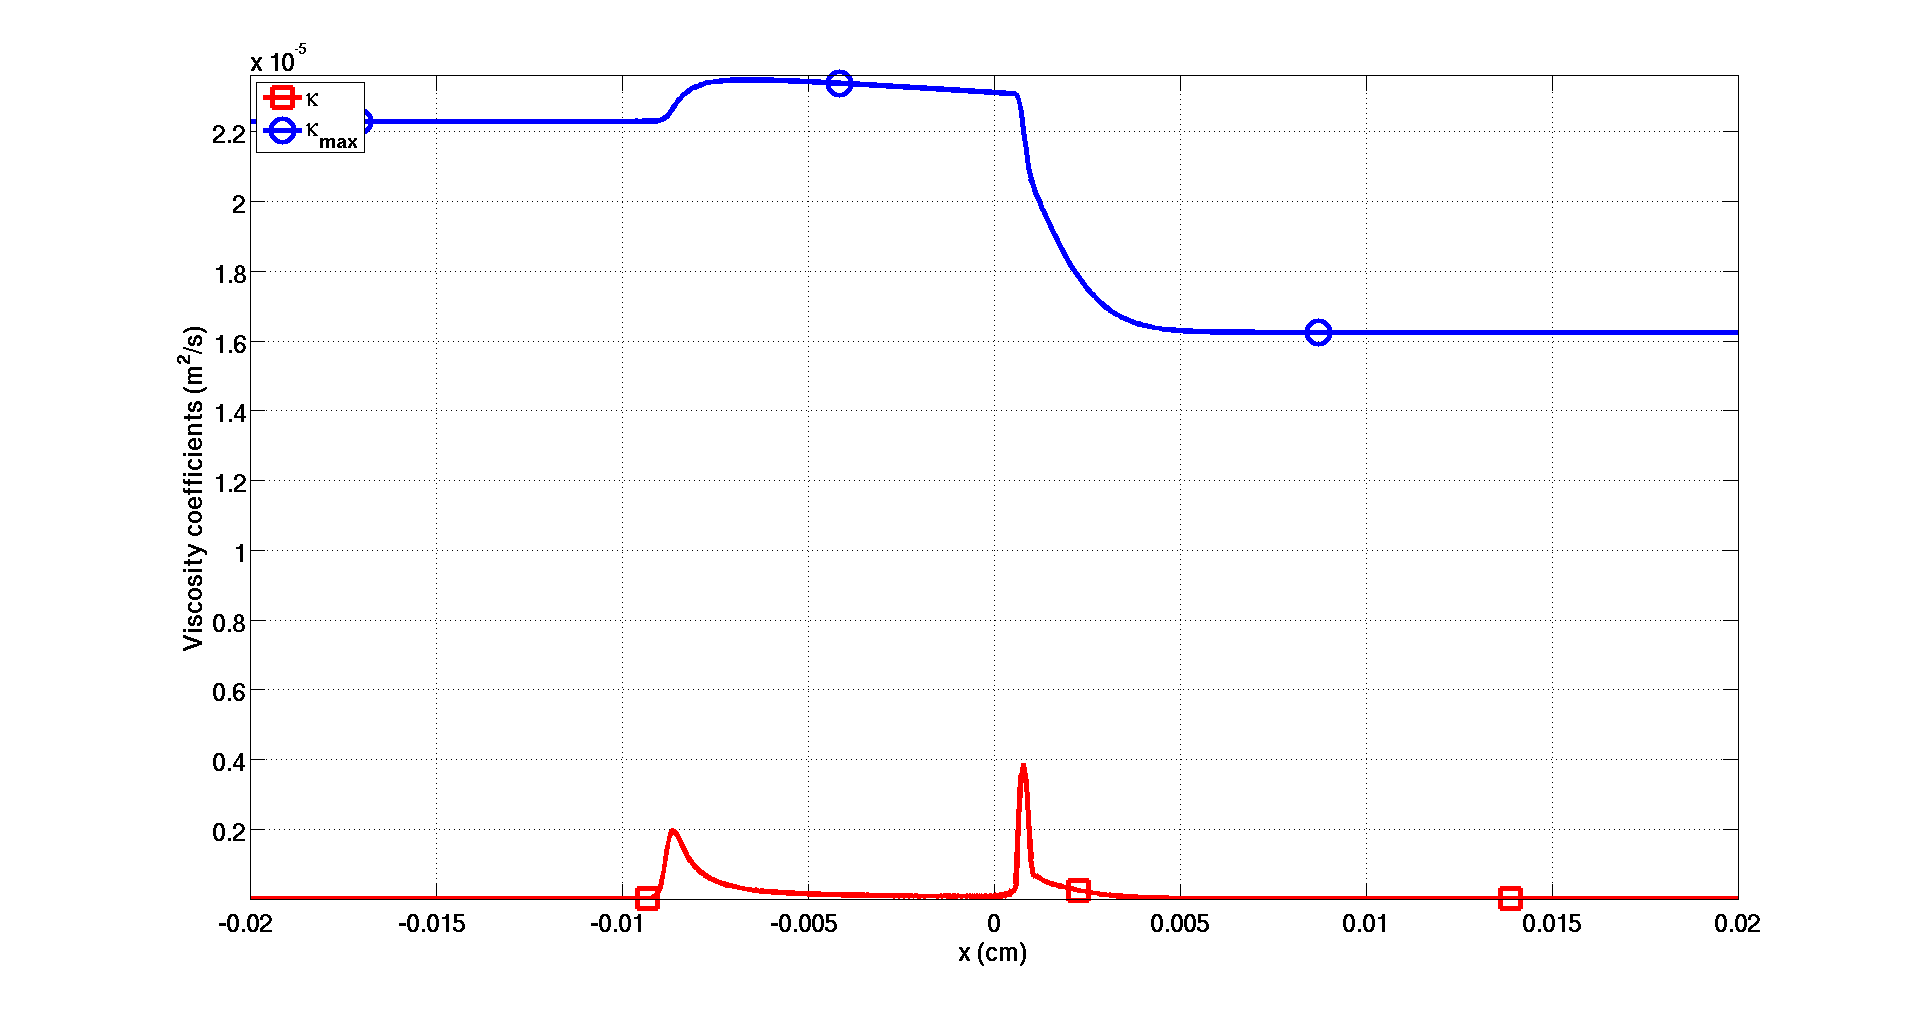
\includegraphics[width=0.99\textwidth]{figures_new_results/mach-3-temp-dpt-xs-viscosity-2000.png}
\end{figure}

\end{frame}
%%%%%%%%%%%%%%%%%%%%%%%%%%%%%%%%%%%%%%%%%%%%%%%%%%%%%%%%%%%%%%%%%%%%

%%%%%%%%%%%%%%%%%%%%%%%%%%%%%%%%%%%%%%%%%%%%%%%%%%%%%%%%%%%%%%%%%%%%
%%%%%%%%%%%%%%%%%%%%%%%%%%%%%%%%%%%%%%%%%%%%%%%%%%%%%%%%%%%%%%%%%%%%
\subsection{Summary}
%%%%%%%%%%%%%%%%%%%%%%%%%%%%%%%%%%%%%%%%%%%%%%%%%%%%%%%%%%%%%%%%%%%%
%%%%%%%%%%%%%%%%%%%%%%%%%%%%%%%%%%%%%%%%%%%%%%%%%%%%%%%%%%%%%%%%%%%%

%%%%%%%%%%%%%%%%%%%%%%%%%%%%%%%%%%%%%%%%%%%%%%%%%%%%%%%%%%%%%%%%%%%%
\begin{frame}

\begin{block}{Conclusions on viscous regularization of the GRH equations}
\begin{itemize}
\item Extended the entropy-viscosity method to the \hili{full} Grey Radiation-Hydrodynamic equations.
\item Verified the entropy minimum principle for the regularized equations GRHD.
\item Viscous regularization scales appropriately in the equilibrium-diffusion limit.
\item Numerical results are in excellent agreement with semi-analytical solutions.
\end{itemize}
\end{block}

\begin{block}{Outlook}
\begin{itemize}
\item Multi-D.
\item Replace radiation diffusion with $S_n$ radiation transport.
\item Switch solution technique to IMEX (implicit for radiation, explicit for hydro).
\item Other spatial discretization (DGFEM).
\item FCT (second part of the talk)
\end{itemize}
\end{block}

\end{frame}
%%%%%%%%%%%%%%%%%%%%%%%%%%%%%%%%%%%%%%%%%%%%%%%%%%%%%%%%%%%%%%%%%%%%

%%%%%%%%%%%%%%%%%%%%%%%%%%%%%%%%%%%%%%%%%%%%%%%%%%%%%%%%%%%%%%%%%%%%
%%%%%%%%%%%%%%%%%%%%%%%%%%%%%%%%%%%%%%%%%%%%%%%%%%%%%%%%%%%%%%%%%%%%
\section{FCT for radiation transport }
%%%%%%%%%%%%%%%%%%%%%%%%%%%%%%%%%%%%%%%%%%%%%%%%%%%%%%%%%%%%%%%%%%%%
%%%%%%%%%%%%%%%%%%%%%%%%%%%%%%%%%%%%%%%%%%%%%%%%%%%%%%%%%%%%%%%%%%%%

%%%%%%%%%%%%%%%%%%%%%%%%%%%%%%%%%%%%%%%%%%%%%%%%%%%%%%%%%%%%%%%%%%%%%%%%%%%%%%%%%
\begin{frame}{FCT for radiation transport }

\begin{block}{Motivation: solution positivity}
\begin{itemize}
\item Solution techniques for radiation transport can produce negative fluxes for discretization orders greater than 1
\item Lumping (mass and gradient lumping) can increase robustness of the solution, but negativities persist
(\tcb{DG high order with P. Maginot})
\item Ultimately, one needs a nonlinear process to ensure positivity of the solution (for methods of order $> 1$)
(\tcb{CSZ for 2D linear and 2D bilinear DG, P. Maginot})
\end{itemize}
\end{block}

\begin{block}{Proposed new concept}
\begin{itemize}
\item Apply Flux-Corrected Techniques (FCT) to radiation transport
\item Today, a status update of our work:
\begin{itemize}
\item FCT + entropy-viscosity for transport (EV as high-order component of the FCT algorithm)
\item Explicit and implicit time discretizations
\item Only \tcb{CFEM} results but extension to \tcr{DG} is planned. 
\item Coding done with FEM library \tcm{deal.ii}
\end{itemize}
%New concept, EV+FCT for transport. Only CFEM results but extension to DG is planned. Need a viscosity-based method to have a failsafe, low-order, strictly non-negative method. Deal.ii
%Extra difficulty: IMPLICIT time-stepping for transport.
\end{itemize}
\end{block}

\end{frame}
%%%%%%%%%%%%%%%%%%%%%%%%%%%%%%%%%%%%%%%%%%%%%%%%%%%%%%%%%%%%%%%%%%%%%%%%%%%%%%%%%

%%%%%%%%%%%%%%%%%%%%%%%%%%%%%%%%%%%%%%%%%%%%%%%%%%%%%%%%%%%%%%%%%%%%%%%%%%%%%%%%%
\subsection{FCT Introduction}
%%%%%%%%%%%%%%%%%%%%%%%%%%%%%%%%%%%%%%%%%%%%%%%%%%%%%%%%%%%%%%%%%%%%%%%%%%%%%%%%%
\begin{frame}{Introduction to Flux-Corrected Transport (FCT)}

\begin{itemize}
   \item Initially developed in 1973 for finite difference discretizations of
      transport/conservation law problems and recently applied to finite element
      method.
   \item Works by adding conservative fluxes to \tcr{satisfy physical bounds on the
      solution}.
   \item Employs a \tcr{high-order} scheme and a \tcb{low-order, monotone} scheme.
   \item Low-order scheme acts as a \tcb{fail-safe} in regions that risk formation
     of spurious oscillations.
   \item Defines a \emph{correction}, or \tcr{\emph{antidiffusion}}, flux, which
      when added to the low-order scheme, produces the \tcr{high-order} scheme
      solution.
   \item \tcm{Limits this correction} flux to enforce the physical bounds imposed.
\end{itemize}

\end{frame}
%%%%%%%%%%%%%%%%%%%%%%%%%%%%%%%%%%%%%%%%%%%%%%%%%%%%%%%%%%%%%%%%%%%%%%%%%%%%%%%%%

%%%%%%%%%%%%%%%%%%%%%%%%%%%%%%%%%%%%%%%%%%%%%%%%%%%%%%%%%%%%%%%%%%%%%%%%%%%%%%%%%
%\section{Explicit discretization}
%\subsection{Radiation Transport Model}
%%%%%%%%%%%%%%%%%%%%%%%%%%%%%%%%%%%%%%%%%%%%%%%%%%%%%%%%%%%%%%%%%%%%%%%%%%%%%%%%%
\begin{frame}{Radiation Transport Model}

\begin{itemize}
  \item Consider the following model for radiation transport:
    \begin{equation}\label{eq:rad_transport}
      \frac{1}{\speed}\ppt{\angularflux}
        + \directionvector\cdot\nabla\angularflux(\x,\directionvector,E,t)
        + \totalcrosssection(\x,E)\angularflux(\x,\directionvector,E,t)
        = \radiationsource(\x,\directionvector,E,t) \eqp
    \end{equation}
  \item Consider a more general case of a scalar conservation law:
    \begin{equation}
      \pd{\scalarsolution}{t} + \nabla\cdot\consflux(\scalarsolution)
      + \reactioncoef(\x)\scalarsolution\xt
      = \scalarsource\xt \eqp
    \end{equation}
  \item Radiation transport fits this model with the following substitutions:
\[
  \scalarsolution\rightarrow\angularflux
  \eqc \quad
  \consflux(\angularflux)\rightarrow\speed\directionvector\angularflux
  \eqc \quad
  \reactioncoef\rightarrow\speed\totalcrosssection
  \eqc \quad
  \scalarsource\rightarrow\speed\radiationsource
  \eqp
\]
\end{itemize}

\end{frame}
%%%%%%%%%%%%%%%%%%%%%%%%%%%%%%%%%%%%%%%%%%%%%%%%%%%%%%%%%%%%%%%%%%%%%%%%%%%%%%%%%

%%%%%%%%%%%%%%%%%%%%%%%%%%%%%%%%%%%%%%%%%%%%%%%%%%%%%%%%%%%%%%%%%%%%%%%%%%%%%%%%
\subsection{Discretization}
%%%%%%%%%%%%%%%%%%%%%%%%%%%%%%%%%%%%%%%%%%%%%%%%%%%%%%%%%%%%%%%%%%%%%%%%%%%%%%%%
\begin{frame}{Discretization}

\begin{itemize}
   \item The simplest time discretization is forward Euler (FE), which gives the
      discrete system
   \begin{equation}
      \consistentmassmatrix\frac{\solutionvector^{n+1}-\solutionvector^n}
        {\dt} + \ssmatrix\solutionvector^n = \ssrhs^n \eqc
   \end{equation}
   where (CFEM approximation):
   \begin{equation}
      \approximatescalarsolution\xt = \sum\limits_{j=1}^N U_j(t) \testfunction_j(\x) \eqc
      \quad \testfunction_j(\x)\in P^1_h
   \end{equation}

   \begin{equation}
     M\ij^C \equiv \int\limits_{\support\ij}
       \testfunction_i(\x) \testfunction_j(\x) d\x \eqc
   \end{equation}
   \begin{equation}
     A\ij \equiv \int\limits_{\support\ij}\left(
       \mathbf{v}\cdot\nabla\testfunction_j(\x) +
		\reactioncoef(\x)\testfunction_j(\x)\right)\testfunction_i(\x) d\x \eqc
   \end{equation}
   \begin{equation}
      b_i^n \equiv \int\limits_{S_i} q(\x,t^n)\testfunction_i(\x) d\x \eqp
   \end{equation}
\end{itemize}

\end{frame}

%%%%%%%%%%%%%%%%%%%%%%%%%%%%%%%%%%%%%%%%%%%%%%%%%%%%%%%%%%%%%%%%%%%%%%%%%%%%%%%%%
\subsection{Low-Order Scheme}
%%%%%%%%%%%%%%%%%%%%%%%%%%%%%%%%%%%%%%%%%%%%%%%%%%%%%%%%%%%%%%%%%%%%%%%%%%%%%%%%%
\begin{frame}{Low-Order Scheme}

\begin{itemize}
   \item To get the \tcm{low-order} scheme, one does the following:
   \begin{itemize}
      \item Lumps the mass matrix:
        $\consistentmassmatrix\rightarrow\lumpedmassmatrix$.
      \item Adds a low-order diffusion operator:
        $\ssmatrix \rightarrow \ssmatrix+\loworderdiffusionmatrix$.
   \end{itemize}
   \item This gives the following, where $\solutionvector^{L,n+1}$ is the
     low-order solution:
   \begin{equation}
   \boxed{
      \textcolor{secondarycolorheavy}{\lumpedmassmatrix}
        \frac{\solutionvector^{L,n+1}-\solutionvector^n}{\dt}
        + (\ssmatrix + \textcolor{secondarycolorheavy}{\diffusionmatrix^L})
          \solutionvector^n = \ssrhs^n \eqp
   }
   \end{equation}
   \item Diffusion matrix $\diffusionmatrix^L$ with local low-order viscosity $\nu_K^L$:
%   is assembled elementwise,
%      where $K$ denotes an element, using a local bilinear form $b_K$ and a
   \begin{equation}
      D\ij^L = \sumKSij \nu_K^L b_K(\testfunction_j,\testfunction_i) \eqp
   \end{equation}
   Several options for the bilinear form $b_K$ 
   \begin{enumerate}
   \item Laplacian
   \item graph Laplacian
   \item edgewise $ij$ diffusion (coined so far $d_{ij}$ by Guermond/Popov)
   \end{enumerate}
   Required properties:
      \begin{equation}
      \sum\limits_j b_K(\testfunction_j, \testfunction_i) = 0 \eqc
   \quad
      b_K(\testfunction_i, \testfunction_i) > 0 \eqp
   \end{equation}

\end{itemize}

\end{frame}
%%%%%%%%%%%%%%%%%%%%%%%%%%%%%%%%%%%%%%%%%%%%%%%%%%%%%%%%%%%%%%%%%%%%%%%%%%%%%%%%%
\begin{frame}{Low-Order Viscosity}

\begin{itemize}
   \item The low-order viscosity is defined as
   \begin{equation}
   \boxed{
     \lowordercellviscosity[\timeindex] \equiv \max\limits_{i\ne j\in\indicescell}
     \frac{\max(0,\ssmatrixletter\ij^\timeindex)}
     {-\mkern-20mu\sumKSij[T]\mkern-20mu\localviscbilinearform{T}{j}{i}}
     \eqp
   }
   \end{equation}
   \item This definition is \tcr{designed to be the smallest number such that} 
   \begin{equation}
      D^L\ij \leq -A\ij, \quad j\ne i \eqp
   \end{equation}
   \item This is used to guarantee that the low-order steady-state matrix
      $\ssmatrix^L=\ssmatrix+\diffusionmatrix^L$ is an M-matrix, i.e., a \tcr{\emph{monotone}} matrix:
      $\ssmatrix^L\solutionvector=\ssrhs \ge 0\Rightarrow \solutionvector\ge 0$.
\end{itemize}

\end{frame}
%%%%%%%%%%%%%%%%%%%%%%%%%%%%%%%%%%%%%%%%%%%%%%%%%%%%%%%%%%%%%%%%%%%%%%%%%%%%%%%%%
\begin{frame}{Discrete Maximum Principle}

\begin{itemize}
   \item In addition to guaranteeing monotonicity and positivity, the low-order
      viscous terms guarantee the following \tcr{discrete maximum principle} (DMP),
      where $U^n_{\max,i} = \max\limits_{j\in\mathcal{I}(S_i)}U^n_j$,
      $U^n_{\min,i} = \min\limits_{j\in\mathcal{I}(S_i)}U^n_j$:
      \begin{equation}
      \boxed{
         W_i^-\leq
         U_i^{L,n+1}\leq
         W_i^+\qquad\forall i \eqc
      }
      \end{equation}
      \begin{equation}
         W_i^\pm \equiv U_{\substack{\max\\\min},i}^n\left(
         1-\frac{\dt}{M_{i,i}^L}
         \sum\limits_j A\ij^L\right)
         + \frac{\Delta t}{M_{i,i}^L}b_i^n \eqp
      \end{equation}
   \item For example, when there is no reaction term or source term, this reduces
      to the following DMP, which implies the scheme is local extremum
      diminishing (LED):
      \begin{equation}
      \boxed{
         U^n_{\min,i}\leq
         U_i^{L,n+1}\leq
         U^n_{\max,i}\qquad\forall i \eqp
      }
      \end{equation}
\end{itemize}

\end{frame}
%%%%%%%%%%%%%%%%%%%%%%%%%%%%%%%%%%%%%%%%%%%%%%%%%%%%%%%%%%%%%%%%%%%%%%%%%%%%%%%%%
\begin{frame}
\frametitle{Low-Order Scheme Results Example}
\framesubtitle{Linear Advection of Discontinuous Wave Front}

\begin{center}
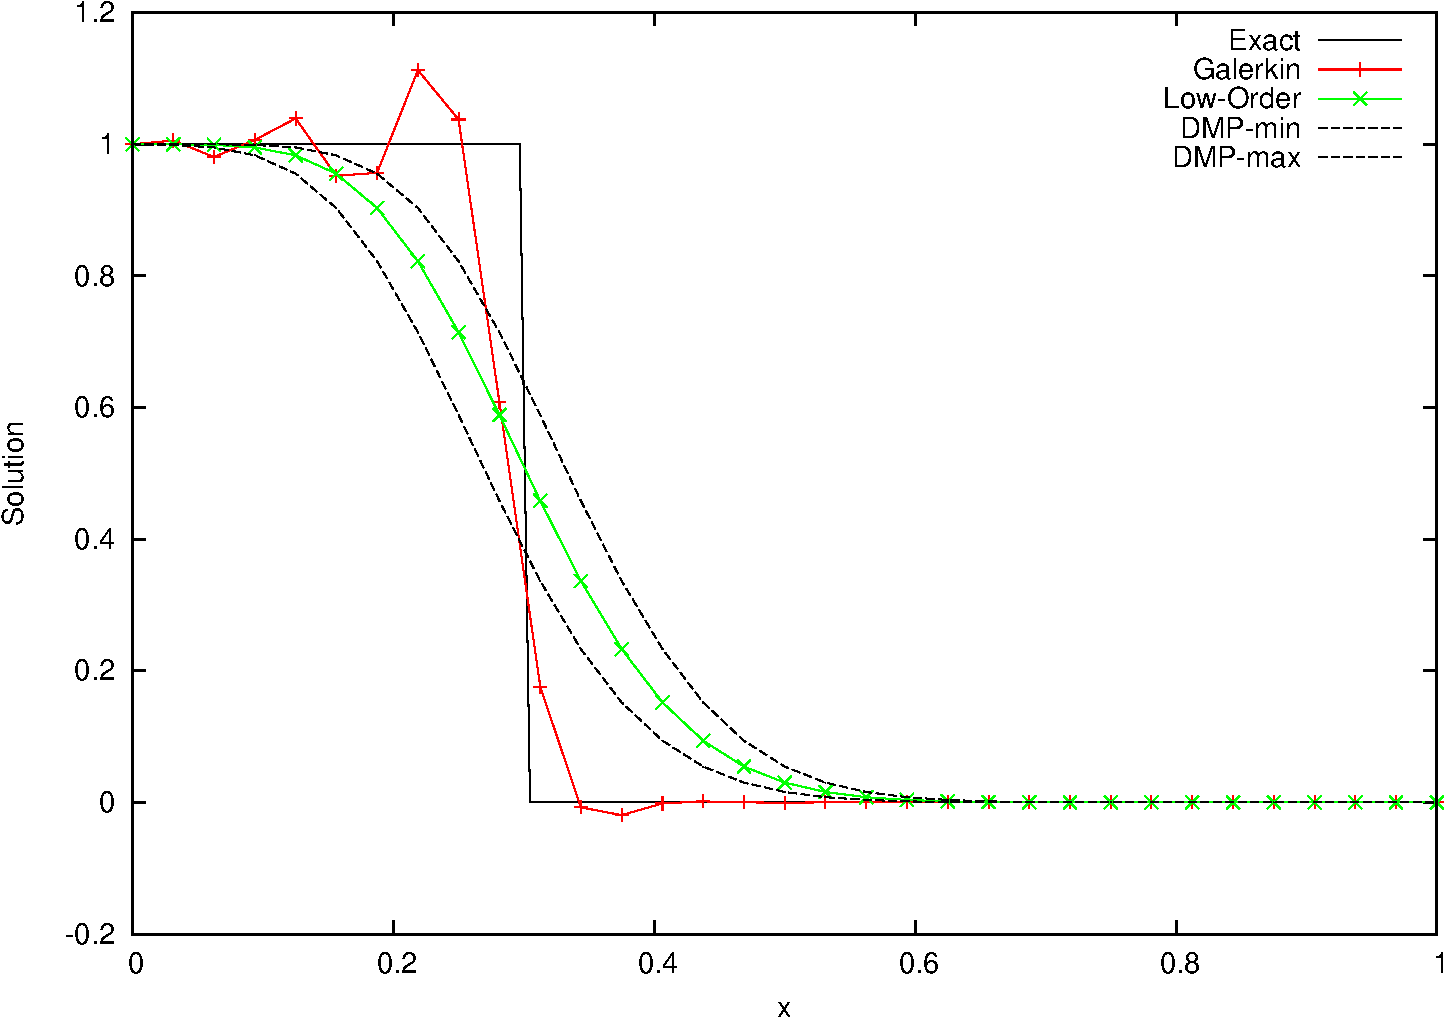
\includegraphics[width=0.85\textwidth]{./figures/advection_low_order.pdf}
\end{center}

\end{frame}
%%%%%%%%%%%%%%%%%%%%%%%%%%%%%%%%%%%%%%%%%%%%%%%%%%%%%%%%%%%%%%%%%%%%%%%%%%%%%%%%%
\subsection{High-Order Scheme}
%%%%%%%%%%%%%%%%%%%%%%%%%%%%%%%%%%%%%%%%%%%%%%%%%%%%%%%%%%%%%%%%%%%%%%%%%%%%%%%%%
\begin{frame}{Entropy Viscosity Definition}

\begin{itemize}
   \item The standard Galerkin CFEM method does not necessarily produce the
      correct weak solution and may even diverge. Even with
      FCT, it would not necessarily converge to the correct, physical
      weak solution, i.e., the \emph{entropy} solution.
      \item \tcr{\underline{Note:}} DG with upwind is mathematically equivalent to a stabilization (viscous regularization), so it may be possible that pure DG (i.e., without EV) may be enough as a high-order scheme.
   \item To converge to the entropy solution, one must ensure that the entropy
      inequality is satisfied:
   \begin{equation}
      R(u) = \pd{\eta}{t}
      + \frac{d\eta}{du}\left(\nabla\cdot(\mathbf{v}u)
      + \reactioncoef u 
      - q \right) \ge 0
   \end{equation}
%         R(u) \equiv \pd{\eta(u)}{t} + \nabla\cdot\mathbf{f}^\eta(u) \leq 0
%      \end{equation}
%      for any convex entropy $\eta(u)$ and corresponding entropy flux
%      $\mathbf{f}^\eta(u)$.
   %\item Note that the entropy inequality in mathematics is flipped from
   %   its definition in thermodynamics, where entropy is a non-\emph{decreasing}
   %   function.
%   \item This \emph{entropy residual} $R(u)$ measures entropy production;
%      where it is positive, the inequality is violated, so the residual
%      should be decreased somehow.
%   \item To enforce the inequality, the entropy viscosity method adds
%      viscosity in proportion to local entropy production, thus decreasing
%      local entropy.
%\end{itemize}
%
%\end{frame}
%%%%%%%%%%%%%%%%%%%%%%%%%%%%%%%%%%%%%%%%%%%%%%%%%%%%%%%%%%%%%%%%%%%%%%%%%%%%%%%%%%
%\begin{frame}{Entropy Viscosity Definition}
%
%\begin{itemize}
%   \item One chooses a convex entropy function $\eta(u)$ such
%   as $\eta(u)=\frac{1}{2}u^2$ and manipulates the
%   conservation law equation to get an entropy residual:
%   \begin{equation}
%      R(u) = \pd{\eta}{t}
%      + \frac{d\eta}{du}\left(\nabla\cdot(\mathbf{v}u)
%      + \reactioncoef u 
%      - q \right) \eqp
%   \end{equation}
   \item Viscosity is set to be proportional to a linear combination
      of the local entropy residual $R_K(u) = \left\|R(u)\right\|_{L^\infty(K)}$
      and entropy jumps $J_F(u)$ across the faces:
      \begin{equation}
         \nu^{\eta}_K \propto c_R R_K(u_h)
         + c_J\max\limits_{F\in\partial K}J_F(u_h) \eqp
      \end{equation}
%   \item In practice, the entropy viscosity becomes the following, where the
%      denominator is just a normalization constant:
%      \begin{equation}
%         \nu^{\eta}_K = \frac{c_R R_K(u_h)
%         + c_J\max\limits_{F\in\partial K}J_F(u_h)}
%         {\|\eta(u_h)-\bar{\eta}(u_h)\|_{L^\infty(\mathcal{D})}} \eqp
%      \end{equation}
\end{itemize}
   
\end{frame}
%%%%%%%%%%%%%%%%%%%%%%%%%%%%%%%%%%%%%%%%%%%%%%%%%%%%%%%%%%%%%%%%%%%%%%%%%%%%%%%%%
\begin{frame}{High-Order Scheme}

\begin{itemize}
   \item The high-order viscosity does not need to be any greater than the
      low-order viscosity:
      \begin{equation}
      \boxed{
         \nu^{H,n}_K = \min(\nu^{L}_K,\nu^{\eta,n}_K) \eqp
      }
      \end{equation}
   \item For the high-order scheme, the mass matrix is not modified; the
      only change is the addition of the high-order diffusion operator
      $\diffusionmatrix^{H,n}$:
      $\ssmatrix \rightarrow \ssmatrix + \diffusionmatrix^{H,n}$:
      \begin{equation}
      \boxed{
        \consistentmassmatrix\frac{\solutionvector^{H,n+1}
          -\solutionvector^n}{\dt} + (\ssmatrix
            + \textcolor{secondarycolorheavy}{\diffusionmatrix^{H,n}})
          \solutionvector^n = \ssrhs^n \eqp
      }
      \end{equation}
   \item The high-order diffusion matrix is computed just as the low-order
      counterpart, except that $\nu^{H,n}_K$ is used instead of $\nu^{L}_K$:
      \begin{equation}
        D\ij^{H,n} = \sumKSij \nu_K^{H,n}
          b_K(\testfunction_j,\testfunction_i) \eqp
      \end{equation}
\end{itemize}

\end{frame}
%%%%%%%%%%%%%%%%%%%%%%%%%%%%%%%%%%%%%%%%%%%%%%%%%%%%%%%%%%%%%%%%%%%%%%%%%%%%%%%%%
\begin{frame}
\frametitle{High-Order Scheme Results Example}
\framesubtitle{Linear Advection of Discontinuous Wave Front}

\begin{center}
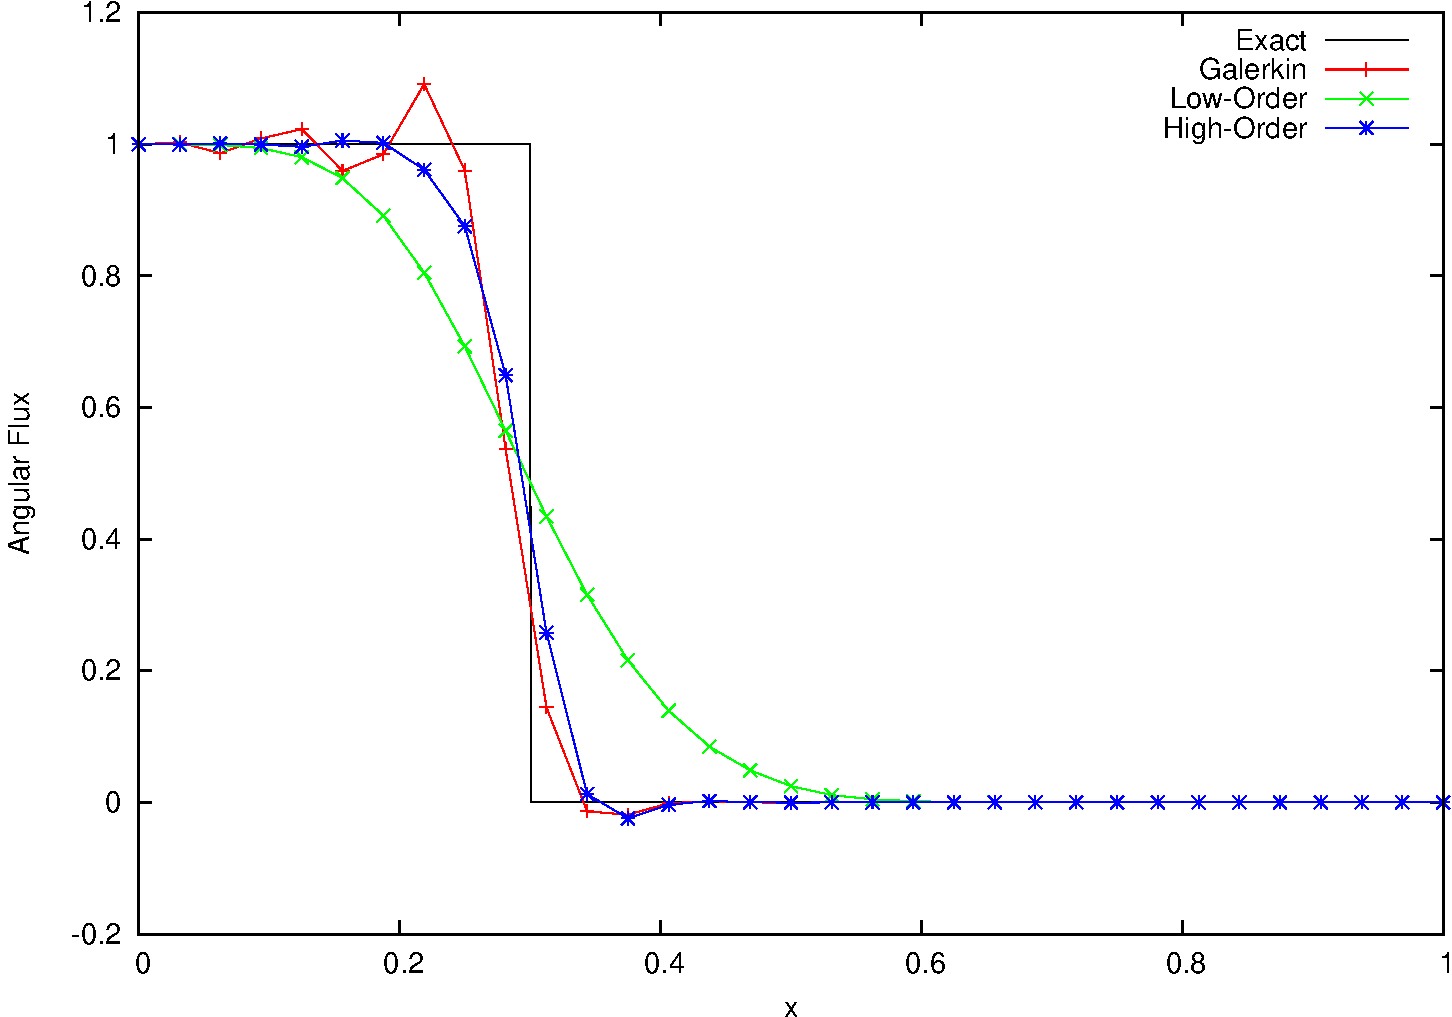
\includegraphics[width=0.8\textwidth]{./figures/advection_high_order.pdf}
\end{center}

\end{frame}
%%%%%%%%%%%%%%%%%%%%%%%%%%%%%%%%%%%%%%%%%%%%%%%%%%%%%%%%%%%%%%%%%%%%%%%%%%%%%%%%%
\subsection{FCT Scheme}
%%%%%%%%%%%%%%%%%%%%%%%%%%%%%%%%%%%%%%%%%%%%%%%%%%%%%%%%%%%%%%%%%%%%%%%%%%%%%%%%%
\begin{frame}
\frametitle{FCT Antidiffusive Flux Definition}

\begin{itemize}
   \item Recall that FCT defines \tcr{antidiffusive correction fluxes}
      from a low-order, monotone scheme to a high-order scheme. Calling
      these fluxes $\correctionfluxvector$, this gives
      \begin{equation}
      \boxed{
        \lumpedmassmatrix\frac{
          \textcolor{secondarycolorheavy}{\solutionvector^{H}}
            -\solutionvector^n}{\dt}
          + (\ssmatrix+\diffusionmatrix^L)\solutionvector^n = \ssrhs^n
          + \textcolor{secondarycolorheavy}{\correctionfluxvector} \eqp
      }
      \end{equation}
   \item Subtracting the high-order scheme equation from this gives the
      definition of $\correctionfluxvector$:
      \begin{equation}
      \boxed{
        \correctionfluxvector \equiv
          -(\consistentmassmatrix-\lumpedmassmatrix)
          \frac{\solutionvector^{H}-\solutionvector^n}{\dt}
          + (\diffusionmatrix^L-\diffusionmatrix^{H,n})\solutionvector^n \eqp
      }
      \end{equation}
   \item Decomposing $\correctionfluxvector$ into internodal fluxes
      $\correctionfluxij$ such that $\sum_j \correctionfluxij =
      \correctionfluxletter_i$,
   \begin{equation}
     \correctionfluxij = -M\ij^C\pr{
       \frac{\solutionletter^{H}_j-\solutionletter^n_j}{\Delta t}
       -\frac{\solutionletter^{H}_i-\solutionletter^n_i}{\Delta t}
       }
       + (D\ij^L-D\ij^{H,n})\pr{\solutionletter^n_j-\solutionletter^n_i} \eqp
   \end{equation}
\end{itemize}

\end{frame}
%%%%%%%%%%%%%%%%%%%%%%%%%%%%%%%%%%%%%%%%%%%%%%%%%%%%%%%%%%%%%%%%%%%%%%%%%%%%%%%%%
\begin{frame}
\frametitle{FCT Scheme Overview}

\begin{itemize}
   \item Recall that the objective of FCT is to limit these antidiffusive
      fluxes to enforce some physical bounds.
   \item The chosen bounds take the form of the DMP satisfied by the
      low-order scheme:
      \begin{equation}
         W_i^-\leq
         U_i^{n+1}\leq
         W_i^+\qquad\forall i \eqp
      \end{equation}
   \item This is achieved by applying a limiting coefficient $L\ij$ to each
      internodal flux $\correctionfluxij$:
      \begin{equation}
      \boxed{
        \lumpedmassmatrix\frac{\solutionvector^{n+1}-\solutionvector^n}{\dt}
          + \ssmatrix^L\solutionvector^n = \ssrhs
          + \textcolor{secondarycolorheavy}{\limitermatrix}
            \cdot\correctionfluxmatrix \eqp
      }
      \end{equation}
   \item Each limiting coefficient is between zero and unity: $0\leq L\ij\leq 1$.
   \begin{itemize}
      \item If all $L\ij$ are zero, then the low-order scheme is produced.
      \item If all $L\ij$ are one, then the high-order scheme is produced.
   \end{itemize}
   \item \tcm{Zalezak's} definitions for the limiter are used here. 
\end{itemize}

\end{frame}
%%%%%%%%%%%%%%%%%%%%%%%%%%%%%%%%%%%%%%%%%%%%%%%%%%%%%%%%%%%%%%%%%%%%%%%%%%%%%%%%%
\begin{frame}
\frametitle{FCT Scheme Results Example}
\framesubtitle{Linear Advection of Discontinuous Wave Front}

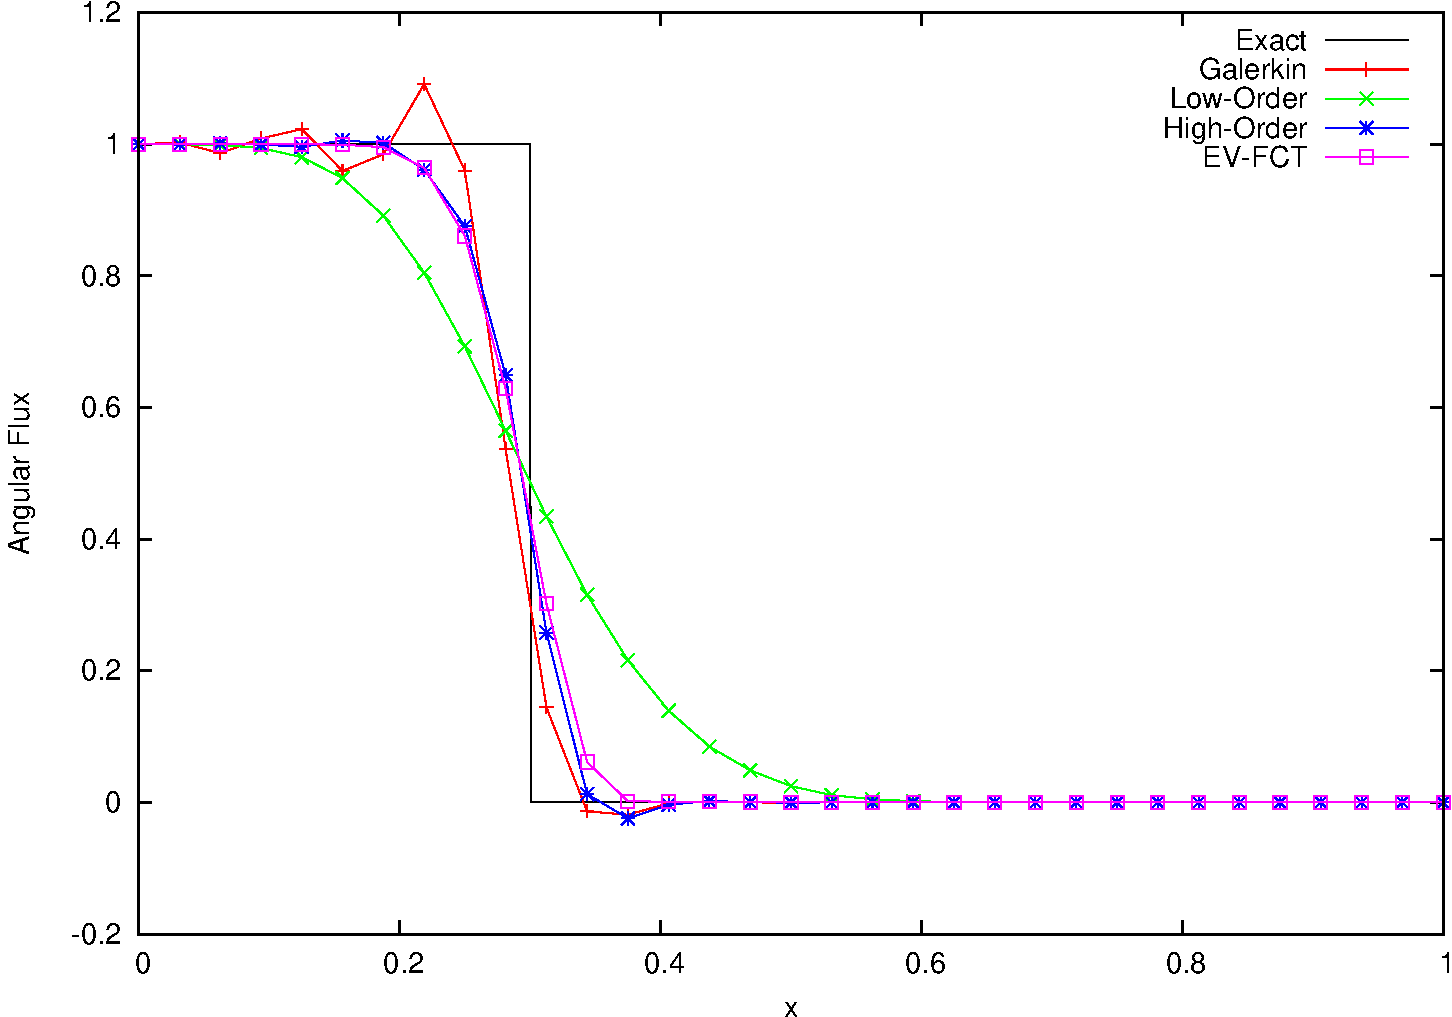
\includegraphics[width=\textwidth]{./figures/advection_FCT.pdf}

\end{frame}
%%%%%%%%%%%%%%%%%%%%%%%%%%%%%%%%%%%%%%%%%%%%%%%%%%%%%%%%%%%%%%%%%%%%%%%%%%%%%%%%%
\subsection{Results}
%%%%%%%%%%%%%%%%%%%%%%%%%%%%%%%%%%%%%%%%%%%%%%%%%%%%%%%%%%%%%%%%%%%%%%%%%%%%%%%%%
\begin{frame}
\frametitle{1-D Test Problem: Applicability to Radiation Transport}
\framesubtitle{Strong Absorber with Source in Left Half of Domain}

\begin{center}
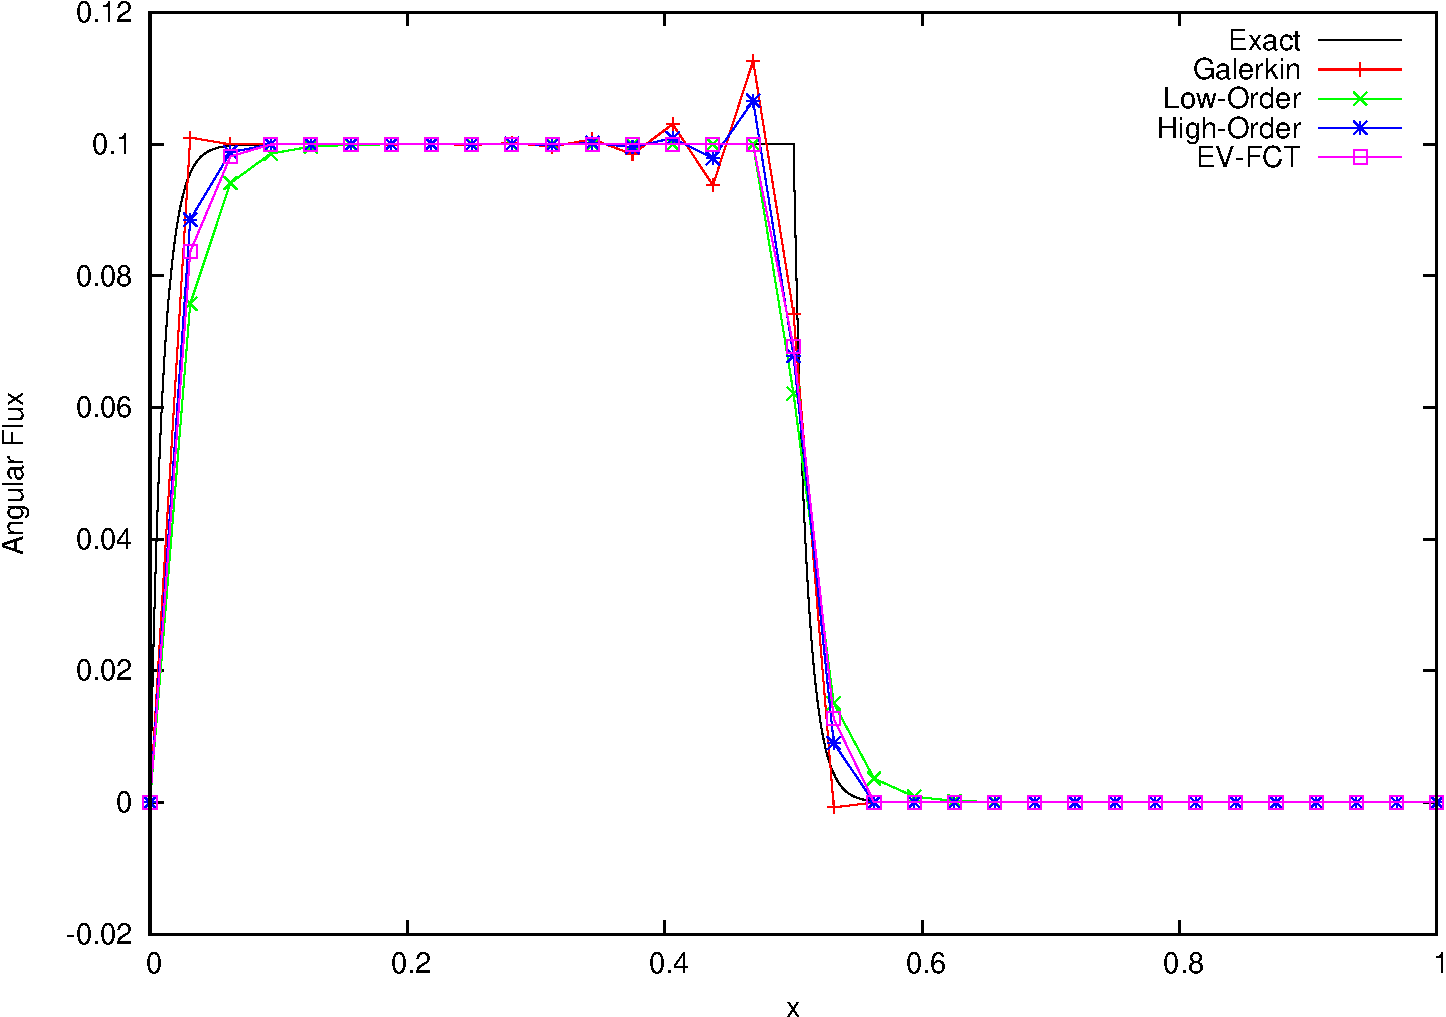
\includegraphics[height=0.8\textheight]{./figures/solutions_source_FE.pdf}
\end{center}

\end{frame}
%%%%%%%%%%%%%%%%%%%%%%%%%%%%%%%%%%%%%%%%%%%%%%%%%%%%%%%%%%%%%%%%%%%%%%%%%%%%%%%%%
\begin{frame}
\frametitle{2-D Test Problem}
\framesubtitle{Normally-Incident Wave from Void to Absorber Quadrant}

\setcounter{subfigure}{0}% Reset subfigure counter
\begin{figure}[h]
   \centering
\subfigure[Exact]{
      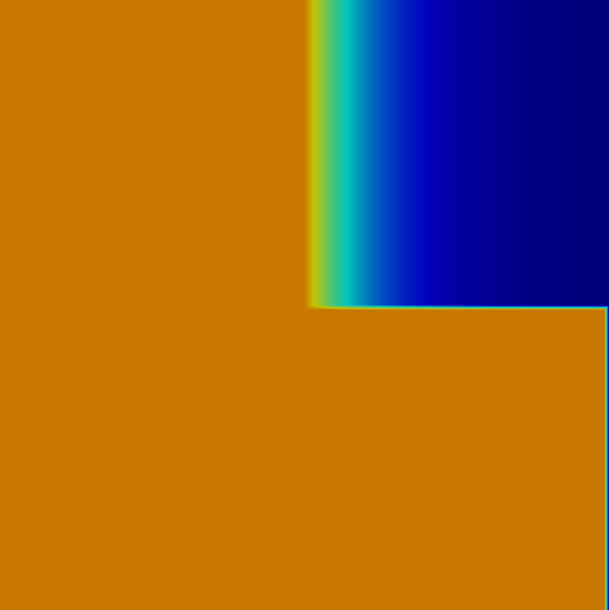
\includegraphics[width=0.25\textwidth]{./figures/exact.png}
}
\subfigure[Galerkin]{
      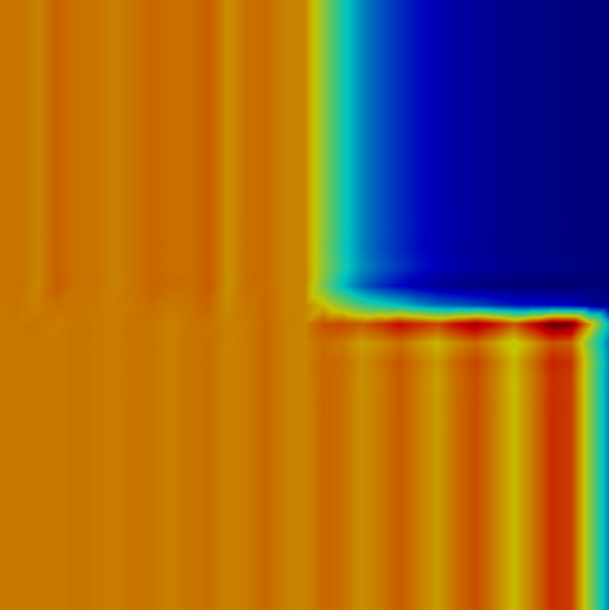
\includegraphics[width=0.25\textwidth]{./figures/Gal.png}
}
\subfigure[Galerkin-FCT]{
      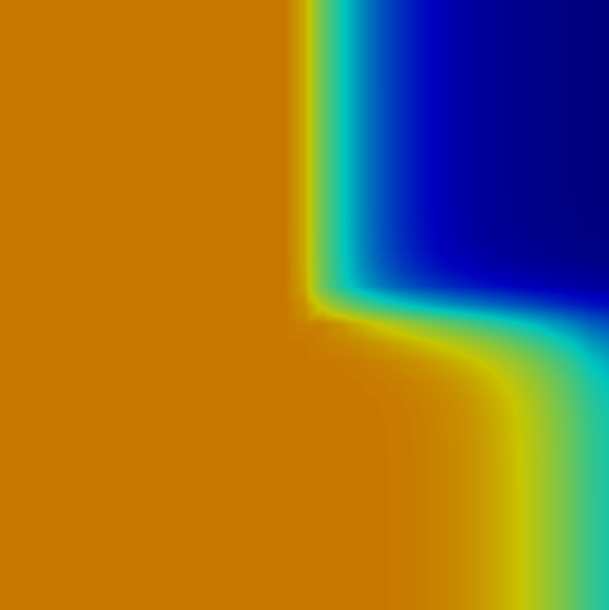
\includegraphics[width=0.25\textwidth]{./figures/GalFCT.png}
}
\subfigure[Low-order]{
      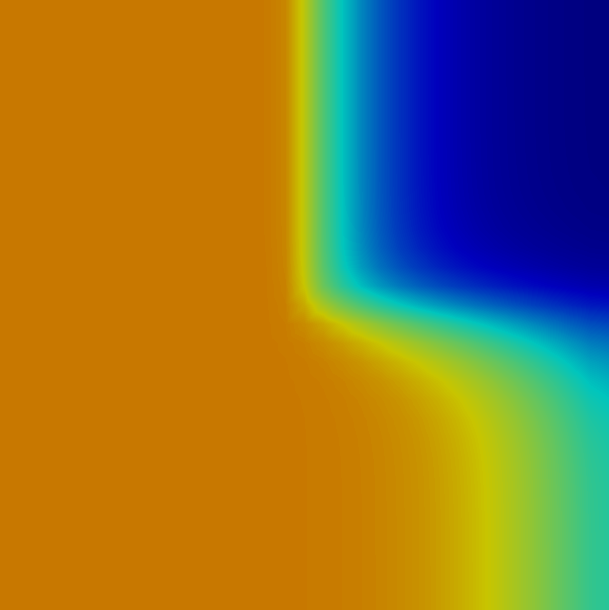
\includegraphics[width=0.25\textwidth]{./figures/low.png}
}
\subfigure[EV]{
      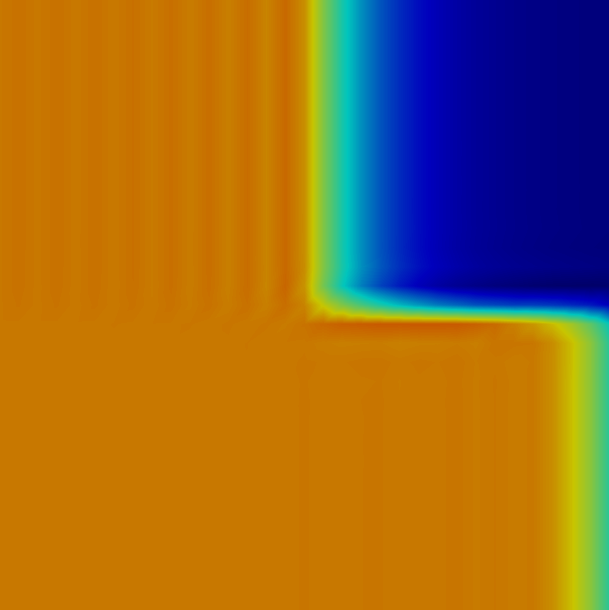
\includegraphics[width=0.25\textwidth]{./figures/EV.png}
}
\subfigure[EV-FCT]{
      \includegraphics[width=0.25\textwidth]{./figures/EVFCT.png}
}
\end{figure}

\end{frame}

%%%%%%%%%%%%%%%%%%%%%%%%%%%%%%%%%%%%%%%%%%%%%%%%%%%%%%%%%%%%%%%%%%%%%%%%%%%%%%%%%



%%%%%%%%%%%%%%%%%%%%%%%%%%%%%%%%%%%%%%%%%%%%%%%%%%%%%%%%%%%%%%%%%%%%%%%%%%%%%%%%%
\begin{frame}
\frametitle{2-D Test Problem}
\framesubtitle{Normally-Incident Wave from Void to Absorber Octant}

% path to figures directory
\newcommand{\FiguresDirnew}{./results/normal_void_to_absorber_2d/images}

% time discretization: "FE" or "SSPRK33"
%\newcommand{\Discretization}{FE}
%
%% type of figure: "figure" for portrait or "sidewaysfigure" for landscape
%%\newcommand{\FigureType}{sidewaysfigure}
%\newcommand{\FigureType}{figure}
%------------------------------------------------------------------------------
\setcounter{subfigure}{0}% Reset subfigure counter

\begin{figure}[h]
   \centering
\subfigure[Exact]{
      \includegraphics[width=0.25\textwidth]{\FiguresDirnew/Exact.png}
}
\subfigure[Low-order]{
      \includegraphics[width=0.25\textwidth]{\FiguresDirnew/low_FE.png}
}
\subfigure[EV]{
      \includegraphics[width=0.25\textwidth]{\FiguresDirnew/EV_FE.png}
}
\subfigure[Galerkin-FCT]{
      \includegraphics[width=0.25\textwidth]{\FiguresDirnew/EVFCT_FE.png} %%????
}
\subfigure[EV-FCT]{
      \includegraphics[width=0.25\textwidth]{\FiguresDirnew/GalFCT_FE.png}
}
\end{figure}

\end{frame}
%%%%%%%%%%%%%%%%%%%%%%%%%%%%%%%%%%%%%%%%%%%%%%%%%%%%%%%%%%%%%%%%%%%%%%%%%%%%%%%%%
%%%%%%%%%%%%%%%%%%%%%%%%%%%%%%%%%%%%%%%%%%%%%%%%%%%%%%%%%%%%%%%%%%%%%%%%%%%%%%%%%

\begin{frame}
\frametitle{2-D Test Problem: Multidimensional Effects}
\framesubtitle{45$^{\circ}$-Incident Wave from Void to Absorber Quadrant}

\setcounter{subfigure}{0}% Reset subfigure counter

\begin{figure}[h]
   \centering
\subfigure[Exact]{
      \includegraphics[width=0.25\textwidth]{./figures/skew_exact.png}
}
\subfigure[Galerkin]{
      \includegraphics[width=0.25\textwidth]{./figures/skew_Gal.png}
}
\subfigure[Galerkin-FCT]{
      \includegraphics[width=0.25\textwidth]{./figures/skew_GalFCT.png}
}
\subfigure[Low-order]{
      \includegraphics[width=0.25\textwidth]{./figures/skew_low.png}
}
\subfigure[EV]{
      \includegraphics[width=0.25\textwidth]{./figures/skew_EV.png}
}
\subfigure[EV-FCT]{
      \includegraphics[width=0.25\textwidth]{./figures/skew_EVFCT.png}
}
\end{figure}

\end{frame}
%%%%%%%%%%%%%%%%%%%%%%%%%%%%%%%%%%%%%%%%%%%%%%%%%%%%%%%%%%%%%%%%%%%%%%%%%%%%%%%%%
\begin{frame}
\frametitle{2-D Test Problem}
\framesubtitle{45$^{\circ}$-Incident Wave from Void to Absorber Octant}

% path to figures directory
%\renewcommand{\FiguresDirnew}{./results/skew_void_to_absorber_2d/images}
%------------------------------------------------------------------------------
\setcounter{subfigure}{0}% Reset subfigure counter

\begin{figure}[h]
   \centering
\subfigure[EV]{
      \includegraphics[width=0.4\textwidth]{./results/skew_void_to_absorber_2d/images/EV_FE_threshold.png}
}
\subfigure[EV-FCT]{
      \includegraphics[width=0.4\textwidth]{./results/skew_void_to_absorber_2d/images/EVFCT_FE_threshold.png}
}
\end{figure}

   Comparison of solutions with 16384 cells for the skew-incident
     absorber test problem showing
     threshold violations: \emph{\tcb{blue}} indicates solution values greater than the
     incoming flux value, and \emph{\tcr{red}} indicates negative solution values.

\end{frame}

%%%%%%%%%%%%%%%%%%%%%%%%%%%%%%%%%%%%%%%%%%%%%%%%%%%%%%%%%%%%%%%%%%%%%%%%%%%%%%%%%
\begin{frame}
\frametitle{1-D Test Problem: Galerkin-FCT Vs. EV-FCT}
\framesubtitle{Left Half: Source in Vacuum, Right Half: No Source in Absorber}

\begin{center}
\includegraphics[height=0.8\textheight]{./figures/sourcevoid_FCT_comparison.pdf}
\end{center}

\end{frame}
%%%%%%%%%%%%%%%%%%%%%%%%%%%%%%%%%%%%%%%%%%%%%%%%%%%%%%%%%%%%%%%%%%%%%%%%%%%%%%%%%

%%%%%%%%%%%%%%%%%%%%%%%%%%%%%%%%%%%%%%%%%%%%%%%%%%%%%%%%%%%%%%%%%%%%%%%%%%%%%%%%%
\begin{frame}
\frametitle{Discrete Maximum Principle Bounds for a Theta-Scheme}

\begin{itemize}
\item Recall the DMP bounds 
  $\DMPbound_i^-\leq \solutionletter_i^{L,\timeindex+1}\leq \DMPbound_i^+$
  for \tcb{explicit} Euler:
      \begin{equation}
         W_i^\pm \equiv U_{\substack{\max\\\min},i}^n\left(
         1-\frac{\dt}{M_{i,i}^L}
         \sum\limits_j A\ij^{L,n}\right)
         + \frac{\Delta t}{M_{i,i}^L}b_i^n \eqp
      \end{equation}
\item In contrast, the DMP bounds for the \tcr{$\theta$ scheme} are implicit:
\begin{subequations}
\begin{multline}\label{eq:theta_bounds}
   \DMPbound_i^\pm
   \equiv \frac{1}{1+\frac{\theta\timestepsize}{\massmatrixletter^L_{i,i}}
     \ssmatrixletter_{i,i}^{L,\timeindex+1}}\Bigg[\pr{1
     - \frac{(1-\theta)\timestepsize}{\massmatrixletter^L_{i,i}}
       \sumj\ssmatrixletter_{i,j}^{L,\timeindex}}
       \solutionletter_{\substack{\max\\\min},i}^\timeindex\\
     - \frac{\theta\timestepsize}{\massmatrixletter^L_{i,i}}
       \sumjnoti\ssmatrixletter_{i,j}^{L,\timeindex+1}
       \solutionletter_{\substack{\max\\\min},i}^{L,\tcr{\timeindex+1}}
     + \frac{\timestepsize}{\massmatrixletter^L_{i,i}}\pr{(1-\theta)
       \ssrhsletter_i^\timeindex + \theta\ssrhsletter_i^{\timeindex+1}}\Bigg] \eqc
\end{multline}
\begin{equation}
  \solutionletter_{\substack{\max\\\min},i}^\timeindex
  = \substack{\max\\\min\limits_{j\in\indices(\support_i)}}
    \solutionletter_j^\timeindex
  \eqc \quad
  \solutionletter_{\substack{\max\\\min},i}^{L,\tcr{\timeindex+1}}
  = \substack{\max\\\min\limits_{j\in\indices(\support_i)}}
  \solutionletter_j^{L,\tcr{\timeindex+1}}
  \eqp
\end{equation}
\end{subequations}
\end{itemize}

\end{frame}
%%%%%%%%%%%%%%%%%%%%%%%%%%%%%%%%%%%%%%%%%%%%%%%%%%%%%%%%%%%%%%%%%%%%%%%%%%%%%%%%%
\begin{frame}
\frametitle{Backward Euler Galerkin FCT for Different CFL Numbers}

\begin{center}
   \includegraphics[width=0.9\textwidth]
     {../../dissertation/content/results/transport/compare_cfl/compare_cfl.pdf}
\end{center}

\end{frame}
%%%%%%%%%%%%%%%%%%%%%%%%%%%%%%%%%%%%%%%%%%%%%%%%%%%%%%%%%%%%%%%%%%%%%%%%%%%%%%%%%
\begin{frame}
\frametitle{Summary}

\begin{block}{Conclusions}
\begin{itemize}
\item FCT applied to the transport equation
\item for explicit (BE, SSP3) and implicit time discretizations (extension to implicit time discretization in progress)
\item We used CFEM (this required EV stabilization in the high-order scheme)
\end{itemize}
\end{block}

\begin{block}{Outlook}
\begin{itemize}
\item Apply the method to \tcr{DG} for transport
\item Possibly no need to stabilize the high-order scheme (\tcr{i.e., do sweeps as usual})
\end{itemize}

\end{block}



\end{frame}

%%%%%%%%%%%%%%%%%%%%%%%%%%%%%%%%%%%%%%%%%%%%%%%%%%%%%%%%%%%%%%%%%%%%
\begin{frame}[noframenumbering]{Thank you}
\label{lastslide}
\centering
Thanks to Jim Ferguson (LANL) for the GRH semi-analytical solutions.\\
Thanks to Jean-Luc Guermond and Bojan Popov (Texas A\&M) for many fruitful discussions.

\begin{figure}
	\centering
	\includegraphics[scale=0.33]{./crunching.png}
\end{figure}

\end{frame}
%%%%%%%%%%%%%%%%%%%%%%%%%%%%%%%%%%%%%%%%%%%%%%%%%%%%%%%%%%%%%%%%%%%%


%%%%%%%%%%%%%%%%%%%%%%%%%%%%%%%%%%%%%%%%%%%%%%%%%%%%%%%%%%%%%%%%%%%%
\begin{frame}[noframenumbering]{Why an upper bound for viscosity?}

\begin{block}{}
Large entropy residual in shocks $\longrightarrow$ large entropy viscosity $\mu_e$ \\
\begin{center}
There is such a thing as too much of a good thing ...\\
{\it Il ne faut point \^{e}tre plus royaliste que le Roy}
\end{center}
\end{block}


\begin{block}{Upper bound for $\mu$}
First-order upwind scheme is monotone but over dissipative. We should not exceed the amount of stabilization that such a scheme provides.\\
\medskip
upwinding = \textcolor{blue}{centered approximation (Galerkin)} $-$ \textcolor{magenta}{numerical diffusion}\\
\underline{Example: linear advection} $\partial_t u + \beta \partial_x u =0$
\be
\beta \frac{u_i - u_{i-1}}{h} = \textcolor{blue}{\beta\frac{ u_{i+1}- u_{i-1}}{2h}} - \textcolor{red}{\frac{\beta h}{2}}
\textcolor{magenta}{\frac{ u_{i+1}-2u_i +u_{i-1}}{h^2}}
\ee
So, the dissipative term is $\frac{\beta h}{2}\partial_{xx} u$
and the first-order viscosity is $\frac{\beta h}{2}$
\end{block}

\begin{block}{First-order viscosity}
\hspace{0.5cm} $\bullet$ scalar conservation law: $\frac{h}{2}|f'(u)|$
\hspace{0.5cm} $\bullet$ system: $\frac{h}{2} \max \left( \text{eig}( \partial_u f) \right) $
\end{block}


\end{frame}
%%%%%%%%%%%%%%%%%%%%%%%%%%%%%%%%%%%%%%%%%%%%%%%%%%%%%%%%%%%%%%%%%%%%


%%%%%%%%%%%%%%%%%%%%%%%%%%%%%%%%%%%%%%%%%%%%%%%%%%%%%%%%%%%%%%%%%%%%
\begin{frame}[noframenumbering]{Manufactured solution: \tcr{equilibrium-diffusion limit}}

\begin{table}[h]
\caption{\label{tbl:table1} L$_2$ norms of the error for for the equilibrium diffusion limit case using a manufactured solution.}
\begin{center}
\begin{tabular}{|c|c|c|c|c|c|c|c|c|c|}
\hline
\textbf{\# of cells} & time step size $(sh)$  & $\mathbf{\rho}$ & \textbf{ratio} & $\mathbf{\rho E}$ & \textbf{ratio} \\ \hline
$20$ & $10^{-1}$ &	 $0.590766$ & NA &  $1.333774$ & NA \\ \hline
$40$ & $5$ $10^{-2}$ & $0.290626$ & $2.03$ &  $0.478819$ & $2.79$ \\ \hline
$80$ & $2.5$ $10^{-2}$ & $0.0959801$ & $3.021$ &  $0.154119$ & $3.11$ \\ \hline
$160$ & $1.25$ $10^{-2}$ & $0.02593738$ & $3.70$ &  $0.0405175$ & $3.80$ \\ \hline
$320$ & $6.25$ $10^{-3}$ & $6.471444$ $10^{-3}$ & $4.00$ & $9.90446$ $10^{-3}$ & $4.09$ \\ \hline
$640$ & $3.125$ $10^{-3}$ & $1.584158$ $10^{-3}$ & $4.01$ & $2.44727$ $10^{-3}$ & $4.04$ \\ \hline
\hline
\textbf{\# of cells} & time step size $(sh)$  & $\mathbf{\epsilon}$ & \textbf{ratio} &  $\mathbf{\rho u}$ & \textbf{ratio} \\ \hline
$20$ & $10^{-1}$ &  $0.00650085$ & NA & $0.910998$ & NA	\\ \hline
$40$ & $5$ $10^{-2}$ &  $0.00124983$ & $5.20$ & $0.4090946$ & $2.23$	\\ \hline
$80$ & $2.5$ $10^{-2}$ &  $0.000262797$ & $4.76$ & $0.125943$ & $3.25$	\\ \hline
$160$ & $1.25$ $10^{-2}$ &  $6.17726$ $10^{-5}$ & $4.25$ & $3.381042$ $10^{-3}$ & $3.72$	\\  \hline
$320$ & $6.25$ $10^{-3}$ & $1.509184$ $10^{-5}$ & $4.09$ & $8.373657$ $10^{-3}$ & $4.04$ \\ \hline 
$640$ & $3.125$ $10^{-3}$  & $3.72548$ $10^{-6}$ & $4.05$ & $2.070538$ $10^{-3}$ & $4.04$ \\ \hline   
\end{tabular}  
\end{center}
\end{table}

\end{frame}
%%%%%%%%%%%%%%%%%%%%%%%%%%%%%%%%%%%%%%%%%%%%%%%%%%%%%%%%%%%%%%%%%%%%


%%%%%%%%%%%%%%%%%%%%%%%%%%%%%%%%%%%%%%%%%%%%%%%%%%%%%%%%%%%%%%%%%%%%
\begin{frame}[noframenumbering]{Manufactured solution: \tcr{streaming limit}}

\begin{table}[h]
\begin{center}
\caption{\label{tbl:table2} L$_2$ norms of the error for for the streaming limit case using a manufactured solution.}
\begin{tabular}{|c|c|c|c|c|c|}
\hline
\textbf{\# of cells} & time step size $(sh)$  & $\mathbf{\rho}$ & \textbf{ratio} & $\mathbf{\rho E}$ & \textbf{ratio} \\ \hline
$20$ &$10^{-1}$& $1.4373$ $10^{-2}$ & NA & $5.88521$ $10^{-1}$ & NA \\ \hline
$40$ & $5.$ $10^{-2}$& $3.760208$ $10^{-3}$ & $3.82$ & $1.4244$ $10^{-1}$ & $4.13$ \\ \hline 
$80$ & $2.5$ $10^{-2}$& $9.91724$ $10^{-4}$ & $3.79$ & $3.2047$ $10^{-2}$ & $4.44$  \\ \hline      
$160$ & $1.25$ $10^{-2}$ & $2.4455$ $10^{-4}$ & $4.06$ & $7.4886$ $10^{-3}$ & $4.28$  \\ \hline     
$320$ & $6.25$ $10^{-3}$ & $6.280715$ $10^{-5}$ & $3.89$ & $1.82327$ $10^{-3}$ & $4.11$ \\ \hline 
$640$ & $3.125$ $10^{-3}$ & $1.57920$ $10^{-5}$ & $3.98$ & $4.50463$ $10^{-4}$ & $4.05$  \\ \hline
$1280$ & $1.5625$ $10^{-4}$ & $3.96096$ $10^{-6}$ & $3.99$ & $1.12061$ $10^{-4}$ & $4.02$ \\ \hline
\hline
\textbf{\# of cells} & time step size $(sh)$  & $\mathbf{\epsilon}$ & \textbf{ratio} &  $\mathbf{\rho u}$ & \textbf{ratio} \\ \hline
$20$ &$10^{-1}$ & $3.82001$ $10^{-1}$ & NA & $2.354671$ $10^{-3}$ & NA \\ \hline
$40$ & $5.$ $10^{-2}$ & $1.21500$ $10^{-1}$ &$3.14$& $6.138814$ $10^{-4}$& $3.84$ \\ \hline
$80$ & $2.5$ $10^{-2}$ & $3.27966$ $10^{-2}$ &$3.70$& $1.74974$ $10^{-4}$ & $3.51$ \\ \hline
$160$ & $1.25$ $10^{-2}$ & $8.38153$ $10^{-3}$ &$3.91$& $3.61297$ $10^{-5}$  & $4.84$ \\ \hline
$320$ & $6.25$ $10^{-3}$ & $2.10925$ $10^{-3}$ &$3.97$& $9.03866$ $10^{-6}$ & $3.99$ \\ \hline
$640$ & $3.125$ $10^{-3}$ & $5.28472$ $10^{-4}$ &$3.99$& $2.25649$ $10^{-6}$ & $4.01$ \\ \hline
$1280$ & $1.5625$ $10^{-4}$ &$1.322268$ $10^{-4}$ &$3.99$& $5.69984$ $10^{-7}$ & $3.95$ \\ \hline
\end{tabular}
\end{center}
\end{table}

\end{frame}
%%%%%%%%%%%%%%%%%%%%%%%%%%%%%%%%%%%%%%%%%%%%%%%%%%%%%%%%%%%%%%%%%%%%


%%%%%%%%%%%%%%%%%%%%%%%%%%%%%%%%%%%%%%%%%%%%%%%%%%%%%%%%%%%%%%%%%%%%
\begin{frame}{Seven-equation two-phase flow model}
\vspace{-3mm}
\begin{block}{with viscous regularization}
\vspace{-3mm}
\begin{subequations}
\begin{align}
  % liquid volume fraction
  \label{eqn:multi-d-7-eqn-liq-vol}
  \frac{\partial \alpha_{k} A}{\partial t} + A\mbold u_{int} \cdot \grad \alpha_{k}
  &- A \mu_P (P_{k} - P_{j}) = \tcr{\div \mbold l_k}
\end{align}
\vspace{-3mm}
\begin{align}
  % liquid mass conservation
  \label{multi-d-7-equ-liq}
  \frac{\partial \left( \alpha \rho \right)_{k} A}{\partial t}
  + \div \left[ (\alpha \rho \mbold u)_k A\right]
  &= \tcr{\div \mbold f_k}
\end{align}
\vspace{-6mm}
\begin{multline}\label{eq:multi-7-eqn-mom}
  % liquid momentum
  \frac{\partial \left( \alpha \rho \mbold u \right)_{k} A}{\partial t}
  + \div \left[ \alpha_{k} A \left( \rho \mbold u \otimes \mbold u + P \mathbb{I} \right)_{k} \right]
  - P_{int} A \grad \alpha_{k} + P_{k} \alpha_{k} \grad A
  \\
  - A \lambda_u (\mbold u_{j} - \mbold u_{k})
  =  \tcr{\div \mathbb{g}_k }
\end{multline}
\vspace{-6mm}
\begin{multline}\label{eq:multi-7-eqn-energy}
  % liquid total energy
  \frac{\partial \left( \alpha \rho E \right)_{k} A}{\partial t}
  + \div \left[ \alpha_{k} \mbold u_{k} A \left( \rho E + P \right)_{k} \right]
  - P_{int} A \mbold u_{int} \cdot \grad \alpha_{k} + \bar{P}_{int} A \mu_P (P_{k} - P_{j})
  \\
  - A \lambda_u \bar{\mbold u}_{int} \cdot (\mbold u_{j} - \mbold u_{k})
  = \tcr{\div \left( \mbold h_k + \mbold u_k \cdot \mathbb{g}_k \right) }
\end{multline}
\end{subequations}
\end{block}
%
\hili{Viscous fluxes}:
%
\begin{equation*}
  \mbold l_k = \tcr{\beta_k} A \grad \alpha_k 
\,, \quad 
  \mbold f_k = \alpha_k A \tcr{\kappa_k} \grad \rho_k + \rho_k  \mbold l_k 
\end{equation*}
\begin{equation*}
\mathbb{g}_k = \alpha_k A \tcr{\mu_k} \rho_k \grad^s \mbold u_k + \mbold f_k \otimes \mbold u_k 
\,, \quad
  \mbold h_k =  \alpha_k A \tcr{\kappa_k} \grad \left( \rho e \right)_k  - \frac{\| \mbold u_k \|^2}{2} \mbold f_k + (\rho e)_k \mbold l_k 
\end{equation*}
%
%where $\beta_k$, $\kappa_k$ and $\mu_k$ are positive phasic viscosity coefficients. 
%
%%
%\begin{align} 
%\alpha_k \rho_k A \frac{Ds_k}{Dt} &- (s_{e})_k \left[\mu_P \frac{Z_k}{Z_k+Z_j} (P_j - P_k)^2 + \lambda_u \frac{Z_j}{Z_k+Z_j} (\mbold u_j -\mbold  u_k)^2 \right. \nonumber
%\\
%&\left. \| \grad \alpha_k \| \frac{Z_k}{\left( Z_k+Z_j \right)^2} \left[ Z_j (\mbold u_j-\mbold u_k)+\frac{\grad \alpha_k}{\| \grad \alpha_k \|}(P_k-P_j)\right]^2 \right] = \nonumber \\
%&\mbold f_k \cdot \grad s_k + \div \left( \alpha_k A \rho_k \kappa_k  \grad s_k \right) 
%- \alpha_k \rho_k A \kappa_k Q_k \nonumber \\
%&+ (s_e)_k \alpha_k A \rho_k \mu_k \grad^s \mbold u_k : \grad \mbold u_k \ ,
%\end{align}

\end{frame}
%%%%%%%%%%%%%%%%%%%%%%%%%%%%%%%%%%%%%%%%%%%%%%%%%%%%%%%%%%%%%%%%%%%%

%%%%%%%%%%%%%%%%%%%%%%%%%%%%%%%%%%%%%%%%%%%%%%%%%%%%%%%%%%%%%%%%%%%%
\begin{frame}{7-equation two-phase flow: shock tube with large relaxation}

\setcounter{subfigure}{0}% Reset subfigure counter

\begin{figure}[H]
\centering
\subfigure[Densities]{
\includegraphics[width=0.31\textwidth]{figures_sem/relaxation_two_phases_density.eps}
}
\subfigure[Pressures]{
\includegraphics[width=0.31\textwidth]{figures_sem/relaxation_two_phases_pressure.eps}
}
\subfigure[Volume fractions]{
\includegraphics[width=0.31\textwidth]{figures_sem/relaxation_two_phases_volume_fraction.eps}
}
\\
\vspace{-3mm}
%
\subfigure[Viscosity $\kappa$, $\mu$ phase 1]{
\includegraphics[width=0.31\textwidth]{figures_sem/relaxation_phase_1_viscosity_kappa_mu.eps}
}
\subfigure[Viscosity $\kappa$, $\mu$ phase 1]{
\includegraphics[width=0.31\textwidth]{figures_sem/relaxation_phase_1_viscosity_kappa_mu.eps}
}
\subfigure[Viscosity $\beta$ (volume fraction)]{
\includegraphics[width=0.31\textwidth]{figures_sem/relaxation_phase_1_beta.eps}
}
\end{figure}


\end{frame}
%%%%%%%%%%%%%%%%%%%%%%%%%%%%%%%%%%%%%%%%%%%%%%%%%%%%%%%%%%%%%%%%%%%%

%%%%%%%%%%%%%%%%%%%%%%%%%%%%%%%%%%%%%%%%%%%%%%%%%%%%%%%%%%%%%%%%%%%%%%%%%%%%%%%%%
\begin{frame}
\frametitle{Local Viscous Bilinear Form}

\begin{itemize}
   \item The local bilinear form is defined as follows, where $\cellvolume$ denotes
      the volume of element $K$, $\mathcal{I}(K)$ is the set of indices
      corresponding to degrees of freedom with nonempty support on $K$, and
      $n_K$ is the cardinality of this set.
   \begin{equation}
      b_K(\testfunction_j, \testfunction_i) \equiv \left\{\begin{array}{l l}
         -\frac{1}{n_K - 1}\cellvolume & i\ne j, \quad i,j\in \mathcal{I}(K)\\
         \cellvolume                   & i = j,  \quad i,j\in \mathcal{I}(K)\\
         0                & i\notin\mathcal{I}(K)\,|\, j\notin\mathcal{I}(K)
      \end{array}\right. \eqp
   \end{equation}
   \item Some properties that result from this definition are
   \begin{equation}
      \sum\limits_j b_K(\testfunction_j, \testfunction_i) = 0 \eqc
   \end{equation}
   \begin{equation}
      b_K(\testfunction_i, \testfunction_i) > 0 \eqp
   \end{equation}
\end{itemize}

\end{frame}
%%%%%%%%%%%%%%%%%%%%%%%%%%%%%%%%%%%%%%%%%%%%%%%%%%%%%%%%%%%%%%%%%%%%%%%%%%%%%%%%%
\begin{frame}
\frametitle{Limiting Coefficients Introduction}

\begin{itemize}
   \item The enforced bounds can be rearranged to bound the limited flux sums:
      \begin{equation}
         Q^-_i \leq \sum\limits_j L\ij \correctionfluxij \leq Q^+_i \eqc
      \end{equation}
      where $Q_i^\pm$ has the following definition:
      \begin{equation}
         Q_i^\pm \equiv M_{i,i}^L\frac{W_i^\pm-U_i^n}{\Delta t}
         + \sum\limits_j A_{i,j}^L U_j^n - b_i \eqp
      \end{equation}
   \item The classic Zalesak limiting strategy starts by separating the
      negative and positive fluxes:
      \begin{equation}
         Q^-_i \leq \sum\limits_{j:\correctionfluxij<0} L\ij \correctionfluxij +
            \sum\limits_{j:\correctionfluxij>0} L\ij \correctionfluxij\leq Q^+_i \eqp
      \end{equation}
      The positive fluxes risk violating $Q_i^+$, and the negative fluxes risk
      violating $Q_i^-$.
\end{itemize}

\end{frame}
%%%%%%%%%%%%%%%%%%%%%%%%%%%%%%%%%%%%%%%%%%%%%%%%%%%%%%%%%%%%%%%%%%%%%%%%%%%%%%%%%
\begin{frame}
\frametitle{Limiting Coefficients Definition}

\begin{itemize}
   \item Zalesak's limiting coefficients assume that
      all positive fluxes into a node $i$ have the same limiting coefficient
      $L^+_i$ and similarly, negative fluxes have the same limiting coefficient
      $L^-_i$:
      \begin{equation}
        Q^-_i \leq L^-_i \correctionfluxletter^-_i
          + L^+_i \correctionfluxletter^+_i \leq Q^+_i \eqp
      \end{equation}
      where
      \begin{equation}
        \correctionfluxletter_i^- \equiv \sum\limits_{j:\correctionfluxij<0}
          \correctionfluxij \eqc \qquad
        \correctionfluxletter_i^+ \equiv \sum\limits_{j:\correctionfluxij>0}
          \correctionfluxij \eqp
      \end{equation}
   \item As a conservative bound for $L^+_i$, contributions from negative fluxes
      are ignored (pretending $L_i^-=0$), giving
      $L^+_i \leq \frac{Q_i^+}{\correctionfluxletter_i^+}$
      and similarly for $L^-_i$ and the lower bound.
\end{itemize}

\end{frame}
%%%%%%%%%%%%%%%%%%%%%%%%%%%%%%%%%%%%%%%%%%%%%%%%%%%%%%%%%%%%%%%%%%%%%%%%%%%%%%%%%
\begin{frame}
\frametitle{Limiting Coefficients Definition (Cont.)}

\begin{itemize}
   \item Then, recalling that limiting coefficients are not greater than unity:
      \begin{equation}
         L_i^\pm \equiv\left\{
            \begin{array}{l l}
               1 & \correctionfluxletter_i^\pm = 0\\
               \min\left(1,\frac{Q_i^\pm}{\correctionfluxletter_i^\pm}\right) &
                 \correctionfluxletter_i^\pm \ne 0
            \end{array}
            \right. \eqp
      \end{equation}
   \item However, to limit fluxes conservatively, limited correction fluxes must
      be equal and opposite:
      \begin{equation}
        L\ij \correctionfluxij = -L_{j,i}
          \MakeUppercase{\correctionfluxletter}_{j,i} \eqp
      \end{equation}
      Since $\correctionfluxij$ happens to be skew symmetric
      ($\MakeUppercase{\correctionfluxletter}_{j,i}=-\correctionfluxij$) due to the
      chosen flux decomposition, the limiting coefficients must be symmetric:
      $L_{j,i} = L\ij$.
\end{itemize}

\end{frame}
%%%%%%%%%%%%%%%%%%%%%%%%%%%%%%%%%%%%%%%%%%%%%%%%%%%%%%%%%%%%%%%%%%%%%%%%%%%%%%%%%
\begin{frame}
\frametitle{Limiting Coefficients Definition (Cont.)}

\begin{itemize}
   \item Thus when deciding the limiting coefficient $L\ij$ for a flux $\correctionfluxij$, 
      one must not only consider the bounds for $i$ but also the bounds for $j$.
      Specifically, a positive flux $\correctionfluxij$ risks violating $Q_i^+$ and $Q_j^-$.
      Putting everything together,
      \begin{equation}
         L\ij \equiv\left\{
            \begin{array}{l l}
               \min(L_i^+,L_j^-) & \correctionfluxij \geq 0\\
               \min(L_i^-,L_j^+) & \correctionfluxij < 0
            \end{array}
            \right. \eqp
      \end{equation}
\end{itemize}

\end{frame}
%%%%%%%%%%%%%%%%%%%%%%%%%%%%%%%%%%%%%%%%%%%%%%%%%%%%%%%%%%%%%%%%%%%%%%%%%%%%%%%%%
\begin{frame}
\frametitle{3-D Test Problem}
\framesubtitle{Normally-Incident Wave from Void to Absorber Octant}

\setcounter{subfigure}{0}% Reset subfigure counter

\begin{figure}[h]
   \centering
\subfigure[Galerkin]{
      \includegraphics[width=0.45\textwidth]{./figures/Gal_3D.png}
}
\subfigure[Galerkin-FCT]{
      \includegraphics[width=0.45\textwidth]{./figures/GalFCT.png}
}
\end{figure}

\end{frame}

%%%%%%%%%%%%%%%%%%%%%%%%%%%%%%%%%%%%%%%%%%%%%%%%%%%%%%%%%%%%%%%%%%%%%%%%%%%%%%%%%
\begin{frame}
\frametitle{1-D Convergence Results (Using FE)}
\framesubtitle{Smooth MMS Problem}

\begin{center}
\includegraphics[height=0.8\textheight]{./figures/convergence_smooth_FE.pdf}
\end{center}

\end{frame}
%%%%%%%%%%%%%%%%%%%%%%%%%%%%%%%%%%%%%%%%%%%%%%%%%%%%%%%%%%%%%%%%%%%%%%%%%%%%%%%%%
\begin{frame}
\frametitle{1-D Convergence Results (Using SSPRK33)}
\framesubtitle{Non-smooth Problem: Linear Advection of Discontinuous Wave Front}

\begin{center}
\includegraphics[height=0.8\textheight]{./figures/convergence_absorber_SSPRK33.pdf}
\end{center}

\end{frame}
%%%%%%%%%%%%%%%%%%%%%%%%%%%%%%%%%%%%%%%%%%%%%%%%%%%%%%%%%%%%%%%%%%%%
%%%%%%%%%%%%%%%%%%%%%%%%%%%%%%%%%%%%%%%%%%%%%%%%%%%%%%%%%%%%%%%%%%%%%%%%%%%%%%%%%
\begin{frame}
\frametitle{1-D Scalar Transport Results}
\framesubtitle{Strong Absorber with Source in Left Half of Domain, 512 Cells}

\begin{center}
   \includegraphics[width=0.8\textwidth]
     {../../dissertation/content/results/transport/source_in_left_half/source_in_left_half_FE_512cells.pdf}
\end{center}

\end{frame}

%%%%%%%%%%%%%%%%%%%%%%%%%%%%%%%%%%%%%%%%%%%%%%%%%%%%%%%%%%%%%%%%%%%%
%%%%%%%%%%%%%%%%%%%%%%%%%%%%%%%%%%%%%%%%%%%%%%%%%%%%%%%%%%%%%%%%%%%%
%%%%%%%%%%%%%%%%%%%%%%%%%%%%%%%%%%%%%%%%%%%%%%%%%%%%%%%%%%%%%%%%%%%%
\end{document}
